\documentclass[12pt,a4paper]{report}

% --- Encoding and fonts ---
\usepackage{iftex}
\ifPDFTeX
  \usepackage[utf8]{inputenc}
  \usepackage[T1]{fontenc}
  \usepackage{mathptmx}
\else
  \usepackage{fontspec}
  \setmainfont{Times New Roman}
  \setsansfont{Times New Roman}
  \setmonofont{Times New Roman}
\fi

% --- Page geometry ---
\usepackage[margin=2.54cm]{geometry}

% --- Line spacing ---
\usepackage{setspace}
\onehalfspacing
\onehalfspacing
\setlength{\parindent}{1.25cm}
\setlength{\parskip}{0pt}

% --- Graphics ---
\usepackage{graphicx}
\usepackage{subcaption}
\usepackage{caption}
\usepackage{float}

\usepackage{tikz}
\usepackage{pgf-pie}
\usetikzlibrary{decorations.pathreplacing, positioning}

\usepackage{indentfirst}
\usepackage{enumitem}
\usepackage{amsmath}
\usepackage{microtype}
\usepackage[htt]{hyphenat}

% --- Tables ---
\usepackage{booktabs}
\usepackage{array}
\usepackage{tabularx}
\usepackage{multirow}
\usepackage{float}
\usepackage{longtable}
\usepackage{caption}
\usepackage{graphicx}
\usepackage{enumitem}
\usepackage{indentfirst}
\usepackage{titlesec}
\usepackage{ltablex}
\keepXColumns

\usepackage[table]{xcolor}

\definecolor{cellyes}{HTML}{EAF3DE}   
\definecolor{cellyesborder}{HTML}{3B6D11} 
\definecolor{cellno}{HTML}{F4F4F2}    
\definecolor{rowhdr}{HTML}{F7F7F5}    
\definecolor{colhdr}{HTML}{2C2C2A}    

\usepackage{pgfplots}
\pgfplotsset{compat=1.18}

\usepackage{pgfplotstable}

\newcommand{\Yes}{\cellcolor{cellyes}\textcolor{cellyesborder}{\textbf{+}}}
\newcommand{\No}{\cellcolor{cellno}\textcolor{gray}{---}}


% --- Paragraph formatting ---
\usepackage{indentfirst}
\setlength{\parindent}{1.25cm}
\setlength{\parskip}{6pt}

% --- Enumeration ---
\usepackage{enumitem}

% --- Hyperlinks (clickable citations) ---
\usepackage{xurl}
\usepackage[
  colorlinks  = true,
  linkcolor   = black,
  citecolor   = black,
  urlcolor    = blue,
  pdfborder   = {0 0 0}
]{hyperref}

% --- Heading formatting ---
\usepackage{titlesec}

%   Chapter: "Chapter N. Title" - 14pt bold, centered
\titleformat{\chapter}[block]
  {\normalfont\fontsize{14}{16.8}\bfseries}
  {Chapter~\thechapter.~}{0em}{}
\titlespacing*{\chapter}{0pt}{0pt}{24pt}

%   Section (1.1, 1.2 ...): 14pt bold, flush left
\titleformat{\section}
  {\normalfont\fontsize{14}{16.8}\bfseries}
  {\thesection}{1em}{}
\titlespacing*{\section}{0pt}{18pt}{8pt}

%   Subsection (1.1.1 ...): 14pt bold italic, flush left
\titleformat{\subsection}
  {\normalfont\fontsize{14}{16.8}\bfseries\itshape}
  {\thesubsection}{1em}{}
\titlespacing*{\subsection}{0pt}{14pt}{6pt}

\captionsetup{font=small, labelfont=bf, justification=centering, singlelinecheck=false}
\captionsetup[figure]{font=small, labelfont=bf, justification=centering, singlelinecheck=false}
\captionsetup[table]{font=small, labelfont=bf, justification=centering, singlelinecheck=false}
\captionsetup[subfigure]{font=small, labelfont=bf, justification=centering, singlelinecheck=false}

\pagestyle{plain}
% --- Bibliography label ---
\renewcommand{\bibname}{Bibliography}

% ============================================================
\begin{document}
% ============================================================
\begin{titlepage}
    \centering
    
    \vspace*{0cm}
    \rule{\textwidth}{0.8pt}\par
    \vspace{0.8cm}
    {\fontsize{18}{22}\selectfont \textbf{Design of a Web Dashboard for Visualizing Road Accident Statistics and Traffic Congestion in the City of Astana}\par}
    \vspace{0.8cm}
    \rule{\textwidth}{0.8pt}\par
    
    \vspace{1.2cm}
    {\large Yelemes Bayan - ST2301 \&  Shaken Ainara - ST2303\par}
    
    \vfill
    
    
\includegraphics[width=0.28\textwidth]{aitu_logo.png}\par
    \vspace{2cm}
    
    {\large School of Intelligent Systems
\par}
    {\large Astana IT University\par}
    
    \vfill
    
    {\normalsize 6B06202 - Smart Technology\par}
    {\normalsize Supervisor: Faizullin Adil\par}
    
    \vfill
    
    {\large JUNE 2026\par}
    {\large ASTANA\par}
\end{titlepage}

\pagenumbering{roman}
\setcounter{page}{1}
% ---------------- ABSTRACT ----------------
\chapter*{Abstract}
\addcontentsline{toc}{chapter}{Abstract}


Road traffic accidents and chronic congestion represent persistent challenges in rapidly
developing urban environments, generating substantial costs to public safety, economic
productivity, and quality of life. In Astana, the capital of Kazakhstan, these challenges
are compounded by the lack of a publicly available and analytically capable information
environment where spatial and temporal patterns in traffic incidents can be explored.
Existing commercial navigation systems offer real-time routing, but they do not maintain
a database of past traffic incidents for research use, are not designed to accept
structured analytical data submissions, and do not provide district-level or
weather-based analytical views.

This thesis describes the design and implementation of \textbf{AstanaSafe} -- a
web-based interactive dashboard for displaying information on traffic accidents and
road congestion in Astana. The system was developed within the framework of a
mixed-methods research design, primarily using qualitative data from the study.
Semi-structured interviews were conducted in January 2026 with 19 participants from
four groups of potential users of traffic information in Astana: transport and road
infrastructure specialists, monitoring and dispatch personnel, urban planners and
academic researchers, and ordinary users, including commuters and drivers.
The interview results showed that traffic data is not aggregated, is not provided in a
convenient spatial format, and does not give accessible historical statistics for
previous accidents. These were the most consistently reported problems across all
groups of potential users.

The implemented system contains an interactive map of the studied area built on
OpenStreetMap (OSM) using the Leaflet.js library. The system also has a module for
crowdsourced incident reporting with typed metadata fields, a set of analytical charts,
including an accident density map, accidents by hour chart, accident severity breakdown
for each district, and weather-correlated incident analysis. In addition, a rule-based
AI safety forecast provides time-of-day risk assessments and predicted danger zones.

The principal contributions of the work are a unified interface for accident and
congestion analysis specifically tailored to the Astana urban environment; structured,
queryable storage of user-submitted incidents enabling longitudinal analysis; integrated
weather correlation as an analytical dimension absent in the reviewed commercial traffic
information systems; and an open-source architecture that can be reused in future
research projects and teaching environments.

\vspace{0.5cm}
\noindent\textbf{Keywords:} traffic accident visualisation, road safety dashboard,
urban traffic analysis, interactive web map, crowdsourced incident reporting,
geospatial data, Astana, Kazakhstan, FastAPI, React.js


\clearpage
% ---------------- LISTS ----------------
\addcontentsline{toc}{chapter}{List of Tables}
\listoftables
\clearpage

\addcontentsline{toc}{chapter}{List of Figures}
\listoffigures
\clearpage

\tableofcontents
\clearpage

\pagenumbering{arabic}
\setcounter{page}{1}

% ---------------- INTRODUCTION ----------------
\chapter*{Introduction}
\addcontentsline{toc}{chapter}{Introduction}

Road safety is one of the most practical measures of a modern city's mobility, public space, and everyday risk management. The city of Astana is particularly significant as the city still expands, new housing areas are emerging, the volume of traffic grows, and the road network is constantly adapting to new travel patterns. Road accidents and traffic congestion are typically considered two different issues: safety is linked to accidents, while travel time and transport efficiency are linked to congestion. In reality, these two problems are connected. A jammed stretch of road can raise the likelihood of risky driving behaviour, and an accident can cause secondary congestion and delay response times instantly \cite{fhwa2015}. Given this, there is a need for tools that integrate accident history, current user reports, spatial context, and operational response information into a single interface to assist in road safety analysis \cite{who2023}.

The subject of the present diploma project is designing a web dashboard for the presentation of road accident statistics and road congestion in the city of Astana. In the project implementation, \textbf{AstanaSafe}, a city decision support system for road safety, is applied. The result is not only a map with accident points, but also a web platform that allows users to explore the location of incidents, when they occur more often, which districts need attention, and how this analysis can be enhanced by reports from users about congestion. Additional operational modules in the system comprise SOS calls, a dispatcher panel, response scenarios, and RoadVision AI for reviewing accidents through video. These modules are added to the main dashboard and demonstrate the integration of analytical information with actual workflows for responding to incidents.

The relevance of the project is determined by the lack of a publicly accessible analytical tool that is focused specifically on Astana and combines several types of road safety information. Commercial navigation systems allow for route planning, but rarely offer a convenient way to access historical accident data, district-level safety markers, clear data processing, or export accident and congestion data for research. Meanwhile, raw geospatial data comes with its own set of challenges in terms of usability without an interface. The KPSSU/DTP public ArcGIS REST layer is structured data that includes information about accidents, including the date of the accident, an accident identifier, an accident type, year, region code, and road surface condition \cite{kpssuDtp}. Before these records can be used within a dashboard, they need to be filtered, cleaned, and transformed. OpenStreetMap data from Geofabrik provides the road and district context, but requires processing into application-level street, intersection, and district datasets \cite{geofabrikKazakhstan}. AstanaSafe fills this void by turning raw geospatial information into visual analytics.

The problem under discussion in this project may be formulated as follows: road accident and congestion data for Astana exist in different forms, but they are not presented through a single responsive web-based decision-making application that enables users to analyze historical data, report new congestion situations, identify hazardous zones, and facilitate basic coordination of responses. This fragmentation hinders the usability of the data for students, researchers, city analysts, drivers, and dispatch-oriented users. It is also challenging to compare districts, understand repeat crash patterns, and link road safety analysis to on-the-road traffic conditions.

The object of the project is urban road safety data and the traffic situation in Astana. The subject of the project is the collection of methods and software tools for the visualization of road accident statistics, traffic congestion, dangerous areas, and road accident response workflows in a web dashboard. The project aims to build and develop a web-based decision support tool, AstanaSafe, designed for analyzing road accident statistics, traffic congestion, hazardous zones, and submitted reports on road safety in Astana.

The following tasks were set to achieve this goal. The problem domain of road accidents, congestion, and dashboard-based traffic analysis was first explored. Secondly, related research and existing traffic information systems were studied in order to identify their usefulness and limitations. Third, semi-structured interviews were conducted with 19 stakeholders representing transport-related, monitoring, planning, research, and everyday driver views to assess their needs. Fourth, the accident data stored in the KPSSU/DTP ArcGIS layer was cleaned and prepared for the system, while the road network data from OpenStreetMap was also prepared. The fifth task was the design of the architecture of AstanaSafe, including the frontend, backend, database, API services, user roles, and analytical modules. Sixth, React, FastAPI, PostgreSQL, Leaflet, Chart.js, and other libraries were used to implement the web dashboard. Seventh, modules for dashboard visualization, analytics, reports, danger zones, district passports, SOS handling, dispatcher workflows, response scenarios, and RoadVision AI were merged into one application. Eighth, the system was evaluated by automated tests in the backend, production build verification, and manual tests in the user interface.

The project is based on the interconnection of applied system design, geospatial data processing, dashboard design, and software testing. The data collection method employed in the research part is literature review, comparative analysis, and semi-structured interviews. The development part is based on an iterative software engineering approach, where the requirements were derived from the problem domain and interview results, the system architecture was designed along a clear frontend-backend separation, and the implemented modules were validated with the functional requirements. Astana accident records were extracted from a large dataset using geospatial processing, and district and road context were prepared from OpenStreetMap data. Data normalization was used to categorize the attributes in the raw accident and traffic reports to be used in visualization, filtering, and risk analysis.

The fundamental approach of the project involves research into aspects of intelligent transport systems, urban traffic safety analysis, geospatial visualization, decision support systems, and dashboard usability. These areas are directly related to the project, as a road safety dashboard is not just for displaying information, but also for helping to interpret it \cite{few2006}. An effective dashboard should make it easy for the user to compare, present patterns at various levels of granularity, and avoid requiring the user to read raw tables before understanding the situation \cite{shneiderman1996}. The concept of AstanaSafe is realized in the form of KPI cards, map markers, heatmap-like views, district summaries, charts, ranked dangerous zones, and report tables. This choice also follows general principles of quantitative information display \cite{tufte2001}. Visual perception requirements were also considered because dashboard elements need to be readable quickly \cite{ware2012}. City decision support systems are closely related to smart city information systems \cite{chourabi2012}.

The practical aspect of the project is the use of the AstanaSafe application. The backend is developed using FastAPI and SQLAlchemy, and the structured data is stored in PostgreSQL. The historical accident data is stored in the \texttt{real\_accidents} table, and user-submitted congestion and incident reports are stored in \texttt{traffic\_reports}. Authentication and roles enable driver, dispatcher, and administrator workflows. The frontend is developed using React and Vite. Interactive maps are provided with Leaflet and React-Leaflet, and analytical visualizations are provided with Chart.js. The application has different user-facing pages such as Dashboard, Analytics, Reports, Danger Zones, District Passport, AI Forecast, SOS-related pages, Dispatcher, Response Scenarios, RoadVision, Account, Settings, and Admin \cite{leafletDocs}.

The other aspect of the project is to incorporate historical and submitted data. The system has a long-term analytical basis in historical accident records and the ability to model the current road pressure using user-submitted traffic reports within the same user interface. This allows the comparison of stable patterns of accidents with more dynamic congestion signals. Another aspect is dangerous zone logic: areas are classified locally by risk levels based on accident density, traffic reports, accident severity, time, weather conditions, and proximity to intersections. The system is not meant to be a substitute for an official transport planning tool or an emergency platform. Its worth lies in being a model of an open and extensible city-specific dashboard which can be used for analysis, education, prototyping, and further development.

The RoadVision AI module is considered an additional module which is added to the main contribution. Its aim is to facilitate the process of reviewing an accident video by associating an uploaded road incident video with a map point, a preliminary event description, detected participants, a timeline, and a draft conclusion. This is not a core component of the diploma project, but demonstrates how the same platform can be extended from statistical visualization to more in-depth analysis of incidents.

The results of the tests validate the working of the implemented project at software level. Automated tests on the backend include AI forecast logic, password reset behavior, spatial risk analysis helpers, and RoadVision processing functions. The project is currently in a state of success with 25 backend tests completed. The production build for the frontend was also successful, confirming that the React application can be built for production. These results do not validate that it is capable of solving all problems that exist in the field of road safety, but indicate that the modules are technically coherent and are ready for demonstration.

The diploma project consists of the following. The introduction gives the meaning, purpose, activity, object, topic, methods, and usefulness of the topic. The problem statement, theoretical background, literature review, and comparative analysis of existing traffic information systems are presented in Chapter 1. Chapter 2 deals with the system analysis and design of the system, including the needs of the stakeholders, sources of data, requirements, architecture, database design, design of the API, and the logic of risk analysis. Chapter 3 discusses the implementation of AstanaSafe, which comprises the main dashboard, analytical pages, reports, risky zones, district passports, user roles, SOS workflow, dispatcher workflow, RoadVision AI, and testing results. The conclusion provides a summary of the results obtained, the practical application of the project, limitations, and potential future avenues for further enhancements.

\clearpage

% ---------------- CHAPTER 1 ----------------
\chapter{Problem Statement and Literature Review}

\section{Description of the Subject Area and Object of the Study}

One of the prerequisite systems that defines the functionality of a city daily is urban transport. It is a link between residential zones and jobs, universities, hospitals, public services, shopping centers, and recreation areas. The impact of poor operation of this system is manifest almost immediately: increased travel time, greater lack of predictability in public transport, poorer emergency response, and higher risk of road traffic accidents. Therefore, the issue of road safety should not be seen merely as a police or transport engineering problem. It is also a data issue, since the decisions made regarding safer roads rely on the clarity of the data gathered, organized, and interpreted around accidents, congestion, dangerous locations, and user reports.

The scope of this diploma project falls within the field of urban road safety, geospatial data treatment, and web-based decision support systems. All of these areas have a particular role. The problem is urban road safety: road accidents, risky intersections, dangerous road conditions, congestion, and delayed response. Geospatial data processing provides the technological foundation for the use of coordinates, districts, streets, intersections, and map layers. These systems are presented to people who do not need to deal with raw data by using a web-based decision support system that renders the information understandable and usable.

This data from around the world validates the importance of this subject area. Despite some progress made in road safety policy and legislation, road traffic deaths continue to be approximately 1.19 million annually, according to the World Health Organization \cite{who2023}. It is a revealing number that reflects the fact that road safety is a systemic problem in cities, and not just a driver problem. The issue is more concrete at the city level: accidents are not uniformly distributed over the road network. They focus around specific intersections, on specific road lengths, at specific times, under specific weather conditions, and at specific traffic volume points \cite{ewing2009}. Due to this, road safety analysis needs to be visualised in space as well as time, and not just presented in terms of general statistics \cite{anderson2009}.

The city of Astana is an appropriate choice for this project because it is a growing capital city with an increasing road network and traffic flow. Roads become overloaded when the population grows, and with changes to roads, construction, and infrastructure, familiar routes can be altered. Under these circumstances, historical accident data is not sufficient. It is also important to know where existing congestion is reported, which districts have the same type of congestion repeatedly, and the ways in which operational modules can enable users to react to incidents. While a static report will indicate accidents, it will not afford the same level of practical insight as a map, a district-level dashboard, or a report table with filters.

The object of the project is urban road safety data and traffic conditions in Astana. This object contains information about historical accidents, road and district locations, user-reported congestion, and information about dangerous zones and response. The implemented system uses the public KPSSU/DTP ArcGIS REST layer for its historical road accident data. The layer includes the DTP feature layer and fields which include the accident type field \texttt{fd1r08p1}, the accident date field \texttt{rta\_date}, the accident record identifier field \texttt{fd1id}, the year field \texttt{yr}, the region code field \texttt{area\_code}, weather-related fields, and the road surface condition field \texttt{fd1r07p1} \cite{kpssuDtp}. This structure is good for analytical processing, but it still needs to be filtered and prepared before it can be used within a city dashboard.

This source data is then used by the local project workflow as the basis to create a more focused Astana dataset. The file \texttt{astana\_dtp.geojson} is the result of filtering the original \texttt{DTP.geojson} by coordinates using \texttt{extract\_astana\_dtp.py}. This yields a dataset of 12,842 accident records for Astana between 2011 and 2026. Then, \texttt{import\_astana\_dtp\_to\_db.py} imports the records that have been created into the \texttt{real\_accidents} table. This processing step is crucial since a national or large regional geospatial layer is too general to meet the objectives of this project. The dashboard should be used in Astana, so the data should be limited to the area of the city and should be structured in a way that is efficient for the backend to query.

Road and district context is created from OpenStreetMap data provided by Geofabrik. The Kazakhstan Geopackage export is an OpenStreetMap export of spatial data in a GIS-friendly format \cite{osmCopyright}. In the project, the Geopackage is utilized to obtain streets, intersections, and district boundaries of Astana. This extra context is required because accident coordinates themselves are not enough to describe the urban context in which an accident occurs. The value of a point on a map can be enhanced by being associated with a district, a nearby road, an intersection, or a known portion of the city. Geofabrik also offers regular updates of Kazakhstan extracts which include the geographically enabled package format, where the process of preparing the extracts can be reproduced \cite{geofabrikKazakhstan}.

The project topic is the visualization of road accident statistics, traffic congestion, dangerous areas, and response workflows in a web dashboard using a set of methods and software tools. This involves frontend interface design, backend API design, database structure, data normalization logic, map visualization, analytical charts, filtering, user roles, and testing protocols. The subject is not limited to visual design. It also encompasses how raw data is converted to information that can inform decisions. A dangerous zone is not just a red dot on a map, for instance. It is created by merging accident density, traffic reports, severity, time, weather conditions, and proximity to intersections.

There are several groups of main users of AstanaSafe. It is important that drivers and other road users have an easy-to-use way to know when there is road pressure and report congestion or incidents. Users who dispatch need a systematic overview of SOS signals, incidents, and responses. Administrators require user and role management. Organized information about accidents and traffic is needed for research, analysis, and study by students, researchers, and urban analysts in order to understand patterns of accidents and traffic across districts, time periods, and road conditions. The various needs account for the different purpose of the system, which is not intended as a single-purpose map but rather as a broader platform for city decision-making.

The issue of the project is the disconnect between available data and meaningful analysis. Accident records can be stored in an official geospatial layer and road data can be stored in OpenStreetMap, but this does not automatically mean that such a layer is useful for an analytical tool \cite{goodchild2007}. If there is no dashboard, the user must download the files, examine raw attributes, install GIS software, and create charts independently. Many educational, analytical, or operational processes are too heavy for this workflow. AstanaSafe fills this gap and gathers maps, charts, reports, risk zones, district views, and user-submitted data into a single web application.

\section{The Problem of Road Accidents and Traffic Congestion in Cities}

\subsection{Road Accidents as an Urban Safety Problem}

One of the most apparent types of risk facing an urban transport system is road traffic accidents. Not only do they impact the occupants of a vehicle involved in a collision, but they also impact emergency services, public transport schedules, other drivers in the vicinity, pedestrians, and the overall reliability of city movements. About 1.19 million people die yearly from road traffic accidents, and road traffic injuries rank first as a cause of death among children and young adults aged between 5 and 29 years \cite{who2023}. As these numbers demonstrate, road safety is a topic that is not just about technical solutions. It relates to public health, urban planning, law enforcement, infrastructure design, and reliable data.

The issue with accidents is more specific at the city level. A road accident is not just a date and a place. It is located within a context such as a street segment, intersection, district, pedestrian crossing, or bridge. It also has a time dimension, including time of day, day of the week, season, and weather. It is also surrounded by infrastructure, such as road surface, visibility, road geometry, traffic lights, public transport lanes, and traffic flows. When these attributes are recorded only as raw data, it is hard to see any patterns that are repeated. For this reason, accident data must be mapped, charted, ranked, filtered, and presented in a table \cite{erdogan2008}.

This is particularly important for Astana, where the city continues to grow and the transport system is undergoing constant changes. As new districts, broad avenues, construction sites, and more private vehicles join the mix, there is potential for the risk of an accident to change over time from one road to another. The dangers of such a city may not be apparent based on one incident. They might only emerge after several years of records are accumulated and plotted on a map, then compared to district boundaries, roadways, crossings, and time periods. The visualization of historical accidents becomes an important part of city road safety analysis.

A second problem is that accident statistics are usually reported in summary form. Aggregated numbers can be helpful for understanding the overall magnitude of the problem, but they are not sufficient for operational or local analysis. A yearly total does not indicate whether crashes are occurring in a particular area near an intersection, whether crashes are occurring more often during snow and ice weather conditions, or whether crashes are occurring more often in one district than in another. A dashboard can fill this gap by maintaining a connection between the single accident record and its analytical meaning. In AstanaSafe, accidents are not only counted, but they are associated with coordinates, year, road surface state, accident severity category, district context, and map visualization.

\subsection{Traffic Congestion as a Mobility and Safety Issue}

Traffic congestion can be caused by an increase in the demand for road space equaling or surpassing the capacity of the road system. According to the Federal Highway Administration, congestion occurs when there is an imbalance between traffic volume and road capacity \cite{fhwa2015}. This impacts routine driving through slower speeds, more erratic driving times, longer queue times, and more complex route planning. Congestion turns into a quality-of-life issue for an expanding city due to its impact on moving workers to and from work, transportation services, deliveries, emergency response, and access to public services.

There is another direct link between congestion and road safety. Slow traffic is not synonymous with safe traffic. Denser traffic can cause vehicles to swerve into or out of lanes, pass too closely, fail to see adequate space between cars, or attempt to turn unnecessarily to avoid waiting time. Pedestrians and cyclists can sometimes also have to cross more complicated intersections when vehicles block the way or do not use a traffic signal consistently. Meanwhile, an accident can cause non-recurrent congestion as a result of blocking a lane, slowing traffic on nearby lanes, and forcing lane changes. Non-recurrent congestion is frequently attributed to unforeseen temporary reductions of capacity, such as crashes, construction, and special events \cite{fhwa2015}. In practice, accidents and congestion feed on one another.

However, in Astana, congestion data is more complex to analyse because AstanaSafe does not have an external traffic provider. Congestion is not received from a third-party system in the application, but submitted by users through reports. A driver is able to mark a traffic jam or incident, choose metadata, and create a traffic report which is recorded in the \texttt{traffic\_reports} table. This is not intended to be a substitute for professional traffic sensors or commercial traffic data. It is meant for something else: a defined channel to capture flow-related traffic events near the site in the same collection system that already gathers historical accident information.

User-submitted congestion records can include details of the road name, crossroad, type of traffic, weather conditions, duration, traffic volume, road lane closures, notes, district, and time of occurrence that are useful when analyzing congestion. Although it is highly unlikely that reports are 100\% accurate, they can be useful to identify locations where users repeatedly feel traffic is impeding their driving. These reports have greater value in conjunction with historical accident points. A road section with numerous accident records and repeated complaints from users should be targeted more than a road section with only one type of signal \cite{goodchild2007}.

\subsection{The Need for Integrated Accident and Congestion Analysis}

Many traffic information systems suffer from the issue of separating traffic accident data and congestion data. Accident data is typically used as an archive for official analysis, while congestion data is typically used as a real-time navigation layer. This separation is only good for simple route planning, and is not strong enough for city safety analysis. This information may be needed by an agent sitting behind the wheel at the time, and it may be needed by an analyst to determine whether the slow area is historically hazardous. The dispatcher may want to know if the location of the SOS signal was a location with repeated accidents, or whether the section of road where the accident occurred was a section that is typically blocked. These questions involve data integration.

The integrated approach in AstanaSafe is based on the philosophy that road safety is not a collection of individual incidents but a pattern. The long-term layer is formed by historical accident records. The current and semi-current layer is made of user-submitted traffic reports. Spatial meaning is added with road data and district data. These layers are joined with the dashboard interface through maps, charts, reports, danger zones, and district passports. This allows the analysis to shift from an overall question, such as how many accidents occur in the city, toward a more useful question: in which district or road segment action is needed, and under which conditions.

\section{Literature Review and Comparative Analysis of Existing Systems}

\subsection{Research Background}

AstanaSafe is linked to a number of research areas, such as geospatial accident analysis, data visualization using dashboards, traffic information submitted by users, and decision-making support in urban mobility. The project considers road safety data not just as a table, and these directions are important for this reason. The principal function is to convert records of accidents and congestion into values that highlight where risk is focused, how it varies across districts and over time, and which sections of roads need improvement.

Spatial analysis is a fundamental component of most road safety research. Accident points begin to make sense when they are plotted on a map and road sections, intersections, land use, and traffic patterns are compared. Kernel density estimation and other geospatial techniques are used in accident study research for the purpose of identifying accident hot spots. Anderson found that kernel density estimation can be used to indicate hotspots for accidents on roads and then support further classification of these hotspots \cite{anderson2009}. Later work on accident clustering for the network highlighted that road accidents should be studied in the context of the transport network instead of only studying traffic accidents as single nodes in open space \cite{xie2013}. Local spatial statistics are also important for identifying high-risk areas and black zones \cite{anselin1995}. Similar black-zone analysis has also been used to compare local spatial autocorrelation and kernel methods \cite{flahaut2003}. This is very relevant to AstanaSafe, which combines the coordinates of the accident with streets, intersections, dangerous zone indicators, and districts.

Spatial-temporal traffic analytics is another research line that applies to the context. Everything is not static: a road section may become unsafe only at a certain time of year, a district may be safe as an annual total but unsafe at the peak period, and the busiest sections of road, particularly in certain times of year, may repeat themselves. Interactive dashboards facilitate user movement between these levels of analysis without extensive chart or map reconstruction. The utility of dashboard interfaces for exploring spatial-temporal traffic and infrastructure patterns from linked visual components is shown in TA-Dash \cite{tempelmeier2020}. AstanaSafe is built on the same principle: maps, KPI cards, charts, tables in the report, district passports, and danger zone ranking.

\subsection{Review of Existing Traffic Information Systems}

In Kazakhstan and nearby regions, there are already several widely used platforms that provide traffic information to users. The most relevant systems are 2GIS, Yandex Maps, and Google Maps. They were chosen because they are common among drivers and city users, accommodate map navigation, and contain traffic or road event information.

2GIS is a widely used city navigation and directory service. According to its official help files, users can see on the map which roads are closed, what work is being conducted on the roads, where accidents, speed cameras, or other events are located \cite{twogisHelp}. In addition, traffic jams are described on the map, and the 2GIS SDK documentation explains how road events can be reproduced on the map for users \cite{twogisHelp}. This allows 2GIS to be used for navigation and for receiving updates on road events. However, the platform is not designed as an analytical dashboard for past accident analysis. It does not provide a public user interface to analyse and compare the distribution of accidents over a period of time district by district, nor does it provide facilities for exporting user traffic reports in a structured format or for connecting accident history and user-submitted congestion records in a research-oriented database.

Another good navigation traffic layer is available in Yandex Maps. Traffic updates are created with the help of Yandex Maps users, and the map can show the color of road events and positions of traffic jams \cite{yandexMapsHelp}. Users can add events such as accidents, cameras, and road works, including the traffic lane for some events. Information about traffic flow is not entered manually, and the colours of the road sections are determined by the density of the traffic flow \cite{yandexMapsHelp}. For this reason, Yandex Maps works properly for current navigation. It may have less flexibility for this diploma project due to the lack of a reporting structure to derive clear analytics of historical accidents, the absence of dashboards for Astana districts and custom research tables for historical accidents, and the absence of an open backend on which project-specific risk logic can be built.

Google Maps real-time route planning, traffic information, accident reporting, and road closures provide real-time information. According to Google Maps Help, the navigation interface allows users to report incidents such as crashes, traffic jams, roadworks, lane closures and objects on the road \cite{googleMapsNavigation}. These functions are useful for general routing. Google Maps is, however, primarily a consumer navigation product too. It does not have a dashboard for city-level exploration based on the Astana accident layer, it does not show local district-level analytics based on the AstanaSafe accident dataset, and there are no local workflows such as SOS and dispatcher workflows implemented in AstanaSafe.

Existing platforms are good at real-time navigation, but have different purposes compared to AstanaSafe. The former systems support the decision-making of the driver who needs to locate a destination, while AstanaSafe analyzes the level of road safety in a given city. It is a significant difference. A navigation application answers the question of what the route is now. A road safety dashboard answers another question: what are the recurring issues in safety and congestion, and how can they be explored using data?

\subsection{Comparative Analysis of Existing Systems and AstanaSafe}

Compared with 2GIS, Yandex Maps, and Google Maps, existing platforms are much more capable in terms of live routing and coverage of a large number of traffic events on a large scale. 2GIS is mostly navigation-oriented \cite{twogisHelp}. Yandex Maps also focuses on current traffic display \cite{yandexMapsHelp}. Google Maps provides navigation and incident reporting tools for drivers \cite{googleMapsNavigation}. AstanaSafe has a different value. It is city-specific, transparent, and ready to use, and it is based on historical accident data, user-supplied congestion data, indicators at district level, and project workflows. This results in a more suitable application of this system for analysis, education, and prototype decision support applications.

The other constraint of AstanaSafe is that there is no external real-time traffic provider. The system does not automatically identify all of the traffic jams in Astana. Instead, it collects input from a user about congestion and supplies it to a structured analysis input. This makes the system more transparent and lighter; however, it also relies on the reliability and number of reports submitted, as the quality of the congestion analysis will depend on these. The restriction is acceptable for a diploma project, as it is more about the design and implementation of a decision support dashboard, rather than a commercial service for traffic prediction.

\subsection{Novelty of the Proposed System}

It is not just one technology perched on top of another; the novelty of AstanaSafe is a combination of functions. There are currently interactive maps, charts, traffic reports, and roles for users in other systems. The novelty of this project lies in the fact that these are assembled on one platform focused on Astana road safety. This system links historical accident data, the road context from OpenStreetMap, user-generated traffic reports, district analytics, dangerous zone logic, and operational modules.

The first novel aspect is the use of an official public accident data source and development of a specially designed dashboard for Astana. The KPSSU/DTP ArcGIS layer is converted into a local layer and added to the backend database. This enables an accident data file to be examined via a web interface that includes maps and analytics.

The second novel aspect is the blending of historical accident data and self-reported congestion data. This is significant because the history of the incident and current traffic congestion are typically considered separately. In AstanaSafe, both types of data can be viewed as a whole. This aligns with a more functional perspective of road safety, not only because it indicates crash locations in the past, but also because it identifies locations where road users now report congestion or traffic pressure.

The third novelty is the analytical structure based on the district. AstanaSafe provides district-level views as well as ranking of dangerous zones and report tables, which enable comparing parts of the city. This is helpful for an analysis of the area rather than a general map providing road speeds or route offering.

\section{Research Methodology}
\label{sec:methodology}

\subsection{Methodological Approach}

The project adopts a mixed applied method which involves literature search, comparative analysis, semi-structured interviews, geospatial data preparation, system design, implementation, and software testing. This is an appropriate method because the diploma project is neither purely theoretical nor only technical. It involves understanding the road safety problem, identifying user needs, preparing real data, designing the system architecture, implementing the web application, and verifying the result.

A literature review was employed to gain an understanding of the overall problem of road accidents, congestion, geospatial analysis, dashboards, and decision support systems. Existing traffic information systems, such as 2GIS, Yandex Maps, and Google Maps, were analyzed using comparative analysis. This made it possible to identify the difference between navigation-oriented platforms and the analytical dashboard proposed in this project.

Semi-structured interviews were used in the empirical part. This option was chosen as it allows for a balance between prepared questions and the flexibility of discussion. There are different requirements for the type of data for road safety applications depending on the application group: drivers need simple and timely information, dispatchers need status and response information, researchers need structured data, and transport-related users need spatial and temporal patterns. These differences were obtained using semi-structured interviews, which allowed participants to respond in ways that were not restricted.

The engineering part was developed in an iterative manner similar to software development. The results of the problem analysis, comparison of existing systems, and interviews were used to create requirements. Following that, the system architecture was designed, the entities in the database were defined, the API routes were designed, the frontend pages were created, the analytical modules were added, and the testing procedures were prepared. This approach was appropriate because there are multiple interconnected components in the system: dashboard visualization, reports, dangerous zones, district passports, user roles, SOS workflow, dispatcher panel, and RoadVision AI.

\subsection{Semi-Structured Interviews}

In January 2026, semi-structured interviews were conducted with 19 people. These participants were selected for their differing perceptions of road safety data in Astana. The idea was not to survey the whole city, but to find out what specific groups who might use or check a road safety dashboard actually needed.

The people interviewed were divided into four groups. Group A consisted of city transport and road experts, and students who were knowledgeable about transport. Group B consisted of individuals with experience in monitoring and dispatch, understanding incident response and coordination. Group C consisted of urban planners, researchers, students, and academics who are involved with spatial or traffic data. Group D consisted of normal drivers and commuters from Astana.

In each interview, a number of themes were discussed. These covered information sources for road and traffic information, issues with current tools, importance of data, features that participants would like to see in a dashboard, and how AstanaSafe can assist them. The questions were slightly modified for each group, but the core questions remained the same. This enabled comparisons between the groups without losing the natural flow of the interviews.

\begin{table}[H]
\centering
\caption{\centering Composition of interview participants}
\label{tab:interview_sample}
\small
\renewcommand{\arraystretch}{1.25}
\begin{tabularx}{\textwidth}{|p{2.4cm}|X|>{\centering\arraybackslash}p{2cm}|}
\hline
\textbf{Segment} & \textbf{Description} & \textbf{Participants} \\
\hline
A & Transport and road infrastructure specialists or students with relevant transport knowledge & 3 \\
\hline
B & Monitoring and dispatch-oriented users familiar with incident handling & 2 \\
\hline
C & Urban planners, researchers, students, and academic users working with spatial or traffic data & 7 \\
\hline
D & Everyday drivers and commuters in Astana & 7 \\
\hline
\textbf{Total} & \textbf{All stakeholder segments} & \textbf{19} \\
\hline
\end{tabularx}
\end{table}

\subsection{Interview Results}

The interviews revealed that the lack of traffic information is not the real issue, but all the information is distributed. Participants reported using navigation apps, public data, unofficial sources, reports, and their own experiences as current sources of traffic information. None of these sources provides a single view of accident history, traffic jam reports, risks in certain locations, or emergency team response.

The ability to view things visually, such as accident locations, severity, time, and filters by areas, was very important to people in transport. They appreciated the dashboard for infrastructure and for comparing various aspects of the city. Participants who were connected with monitoring and dispatch had a strong interest in knowing the status of an incident, having the precise location, understanding the severity of the incident, and improving team coordination. They felt it would be useful to incorporate SOS capabilities and tools for dispatchers to control operations.

Researchers and students noted the need for historical data that is organized, easily exportable information, and visual tools that reduce manual effort. They indicated that interactive maps, charts, and report tables were helpful for their classes, research, and projects. Drivers and commuters who drive every day wanted something that is easy to understand, makes traffic jams visible, alerts them to accidents, and requires no technical skills to operate.

\subsection{Cross-Cutting Findings}

The system requirements stem from several findings which were determined for two or more different user groups. The most common finding for the different user groups was the requirement for an interactive map. This allows the spatial display of accident data as well as congestion data. Currently, both types of data are often provided to the user in the form of text and numbers. A further requirement determined for the different user groups is the option to filter the displayed data by date, district, type, weather, and severity. Because the users are different, the filtering of the data will also be different.

Thirdly, the information should be presented in a clear and simple manner to enable non-technical users to easily interpret the findings from the system. This places great emphasis on the use of KPI cards, simple and easy-to-understand charts, and map markers together with clear separation between pages or screens of information. In addition, historical records of safety-related information together with user reports enable long-term safety patterns to be related to current pressure on the road. Fifthly, weather and road conditions were found to be important fields of study and analysis from the findings of the participants.

\chapter{System Analysis and Design}

\section{System Requirements and User Roles}

The purpose of AstanaSafe is to create a city-scale decision support system for improving road safety in Astana. In addition to the technical requirements for creating the system, the practical requirements for using the system were also identified in the first chapter. During the interviews, it was found that different users need to view the same road safety situation from different angles. Drivers need simple information about traffic flow and to be able to report accidents and incidents on the road. Researchers need historical data and analyses of the information. Dispatch-oriented users need to know the status of incidents and have the necessary tools to respond to them. Administrators need to manage users and assign them roles and permissions. These requirements define the functional and non-functional requirements of the system.

The system uses role-based access because not all the users will have the same functions within the platform. The driver will only have access to some of the pages within the platform, such as the dashboard, the traffic report form, the account page for drivers, and the SOS functions. The dispatcher will have access to the dispatcher panel, where they can view the SOS incidents, change the status of the SOS reports, and use response scenarios for the dispatched firefighters. The administrator will have access to the admin panel, where they can manage the users and change their roles. This structure makes more sense for the platform than if all the users had the same access because it reflects the roles of each user within the platform.

Based on the roles, it is possible to separate some of the platform's pages into types. For example, pages such as the dashboard, analytics, reports, danger zones, and the district passport are all mainly analytical in purpose and function. Pages such as My SOS, the dispatcher panel, and response scenarios are all operational in their function. Other pages, such as the account, settings, and the admin panel are related to the management of users within the platform. This segregation of functions within the platform makes it more understandable by the users despite the various modules that are contained by the platform.

\section{System Architecture and Data Flow}

AstanaSafe is a client-server web application. The frontend is a single-page application, and the backend is used for data access, validation, authentication, and business logic. The database holds historical accident data as well as user-generated data during the system's operation \cite{chen2012}.

There are four layers of architecture for the system. Starting from the top of the application layers, the client layer consists of the single-page application written with React/Vite for the frontend. The client layer has pages, UI components, maps, charts, forms, language switching, and interactions for the users. The API layer, which is the second layer of the architecture, consists of FastAPI for the backend API. It receives requests from frontend, validates inputs, and then calls the services. It returns the results in JSON format. The third layer for the system architecture is the data layer, which is written with models in SQLAlchemy and a PostgreSQL database for storing the data. The last layer is the analytical/service layer, which contains risk analysis, AI forecast functions, RoadVision processing functions, SOS workflow functions, email service, and other helper functions for roads, districts, and intersections.

A general architecture of AstanaSafe is provided in Figure~\ref{fig:system_architecture}.

The end user interacts with the topmost layer of the architecture, the client layer that is implemented as a single-page web application using React/Vite frontend. The frontend is split into different components following a component-based pattern, where each component represents a certain piece of the application's functionality or feature. Frontend components send requests to the corresponding backend endpoints implemented in the FastAPI API layer. These requests are sent in the form of RESTful API requests, and backend processing happens using the data layer that is implemented through database models and a database storing application data in the form of tables. In addition to data stored in the database, the application also stores and processes data provided in the form of application data files and external/source data files. The application data files contain predefined data for backend and frontend usage, such as data about roads, intersections, districts in the city of Astana, and also predefined data about road accidents. The external/source data files are the KPSSU/DTP accident layer and OpenStreetMap data provided by Geofabrik. These data files are not queried in real time when the user opens the application's dashboard, but rather are processed ahead of time and then served as application data files \cite{kpssuDtp}.

\begin{figure}[H]
\centering
\resizebox{\textwidth}{!}{%
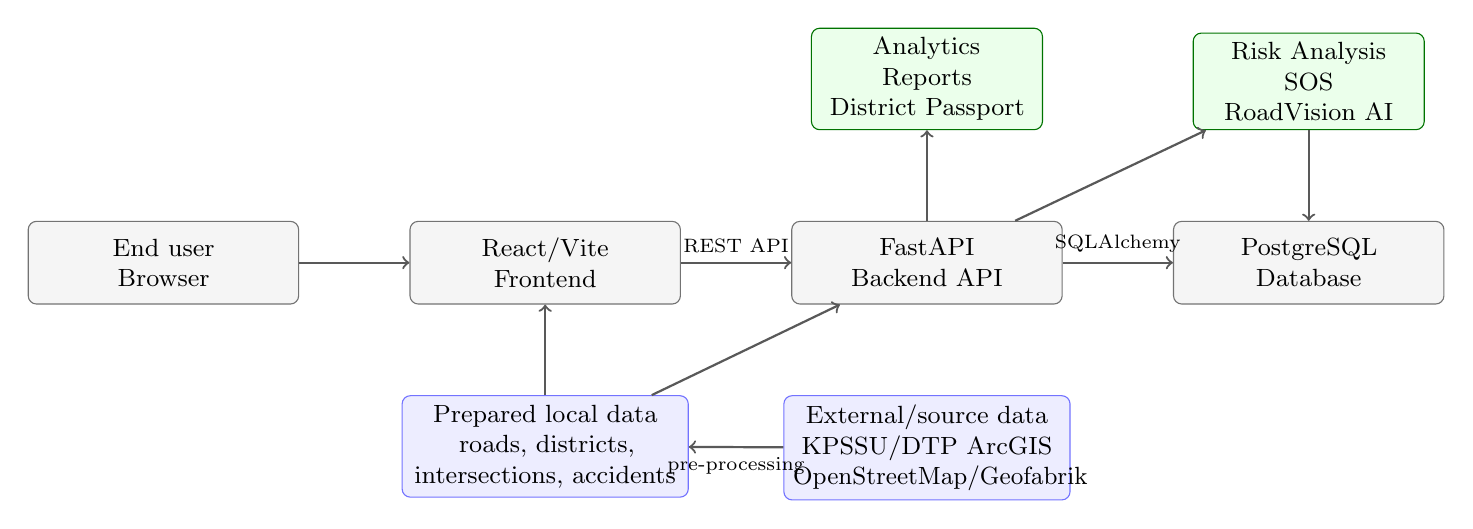
\begin{tikzpicture}[
  node distance=1.15cm and 1.4cm,
  block/.style={
    rectangle,
    draw=black!55,
    rounded corners=3pt,
    align=center,
    minimum height=1.05cm,
    text width=3.2cm,
    fill=gray!8,
    font=\small
  },
  source/.style={
    rectangle,
    draw=blue!55,
    rounded corners=3pt,
    align=center,
    minimum height=1cm,
    text width=3.4cm,
    fill=blue!7,
    font=\small
  },
  module/.style={
    rectangle,
    draw=green!45!black,
    rounded corners=3pt,
    align=center,
    minimum height=0.9cm,
    text width=2.7cm,
    fill=green!8,
    font=\small
  },
  arrow/.style={->, thick, draw=black!65}
]

\node[block] (user) {End user\\Browser};
\node[block, right=of user] (frontend) {React/Vite\\Frontend};
\node[block, right=of frontend] (backend) {FastAPI\\Backend API};
\node[block, right=of backend] (database) {PostgreSQL\\Database};

\node[source, below=of frontend] (localdata) {Prepared local data\\roads, districts, intersections, accidents};
\node[source, below=of backend] (sources) {External/source data\\KPSSU/DTP ArcGIS\\OpenStreetMap/Geofabrik};

\node[module, above=of backend] (analytics) {Analytics\\Reports\\District Passport};
\node[module, above=of database] (operations) {Risk Analysis\\SOS\\RoadVision AI};

\draw[arrow] (user) -- (frontend);
\draw[arrow] (frontend) -- node[above, font=\scriptsize]{REST API} (backend);
\draw[arrow] (backend) -- node[above, font=\scriptsize]{SQLAlchemy} (database);
\draw[arrow] (sources) -- node[below, font=\scriptsize]{pre-processing} (localdata);
\draw[arrow] (localdata) -- (frontend);
\draw[arrow] (localdata) -- (backend);
\draw[arrow] (backend) -- (analytics);
\draw[arrow] (backend) -- (operations);
\draw[arrow] (operations) -- (database);

\end{tikzpicture}
}
\caption{General architecture of AstanaSafe}
\label{fig:system_architecture}
\end{figure}

The frontend is organized according to the routes of the application. Main pages include Dashboard, Analytics, Reports, Danger Zones, District Passport, Forecast, My SOS, Dispatcher, Response Scenarios, RoadVision, Account, Settings, and Admin. These pages are loaded by the routing layer and connected to the main layout. The shared components that are used throughout the application include the sidebar, topbar, authentication modal, map components, filter panel, statistic cards, traffic jam modal, and SOS emergency modal. Using these shared components results in a more cohesive user experience and avoids the duplication of components in different pages within the web application.

For frontend state management, Zustand is used to store the application state. The application store contains the accidents, heatmap points, traffic reports, SOS incidents, selected date, filters, current user, weather, languages, streets, intersections, and modal states. Many pages in the interface use the same data, but present it in a different way. For instance, the Dashboard page, Analytics page, Reports page, Danger Zones page, and District Passport page all use the accident and traffic report data stored in the application store in different ways. This is why it is important to have a centralized store to coordinate the data in the interface.

The backend is organized into separate routers and services. The FastAPI application has routes for accidents, real accidents, traffic reports, roads, risk analysis, SOS incidents, RoadVision, user authentication, and AI functions. The traffic reports router can create, read, and delete traffic reports. The real accidents router exposes the application's historical accident records, processed for easier queries. The risk router provides zone analysis. The SOS router can create incidents, update their status, and make calls over WebSockets.

The database layer is provided by PostgreSQL. The data entities in the system, such as users, districts, accidents, traffic reports, SOS incidents, and password reset tokens, are defined by the SQLAlchemy models. The historical data of real accidents is stored in the \texttt{real\_accidents} table. User-submitted traffic reports of congestion and incidents are stored in the \texttt{traffic\_reports} table. SOS incidents are stored in the \texttt{sos\_incidents} table. The \texttt{users} table contains the data of user accounts and their roles in the system. All entities are separated clearly from each other, which makes it easier to write queries and extend the system later.

The data flow of historical accidents first starts outside the application, where the historical accident data was created by different actors. This data is stored in the KPSSU/DTP ArcGIS REST layer as GeoJSON files. For this application, the file \texttt{DTP.geojson} is stored locally. This GeoJSON file is then filtered for accidents within an approximate bounding box of Astana in an extraction script that produces the GeoJSON file \texttt{astana\_dtp.geojson}. The file \texttt{astana\_dtp.geojson} is then imported into the database using an import script, inserting the data into the \texttt{real\_accidents} table. When the data is requested by the frontend to be displayed on maps, put in tables, create charts, or be used for analytical pages, the backend API is first requested for the historical accidents, and then the data is normalized and returned to the frontend \cite{kpssuDtp}.

As with the SOS incidents, traffic reports are added to the system by users during use of the system. When a driver adds a traffic report, he selects or confirms a location on a map, fills in fields such as road, crossroad, accident category, accident type, weather, duration to pass, traffic flow, number of lanes blocked, free text notes, district, and then submits the form. The form data is then sent from the frontend to the backend by the traffic reports API. After the backend layer has validated the newly added report, it is stored in the PostgreSQL database. After that, the report can be used on the dashboard, analytical pages, reports table, danger zone functionality, and the user's account pages.

The SOS data flow is more of an operational flow than an analytical one. First, a user adds an SOS incident. This incident is filled out with coordinates, urgency, reporter information, and a description. The incident is then stored in the \texttt{sos\_incidents} table and the status of the incident is updated. The dispatcher panel retrieves all SOS incidents from the backend and updates the status of the SOS incidents. In the response scenarios, the status of the SOS incidents is used to represent the current state of processing the SOS incident. The SOS module also has a communication workflow for call-related processes between users and dispatchers. This communication uses WebSocket communication. Hence, the SOS module is not only a static analytical page but also supports operational behavior.

The risk analysis data flow is used to connect historical accident records and risk reports with newly created user reports for locations and defined zones. When a point or a zone is analyzed, backend code searches for close-by real accident records and traffic reports within a given radius, also considering the district and nearby intersections. A risk score is computed based on accident density, traffic volume, distance to intersections, weather, time of day, and recently occurred accidents for that location. The result of a risk analysis is returned as a structured answer to the frontend, including a score, a risk level, all the reasons for the computed risk, all the related interventions, and the geometry of the analyzed zone.

The architecture of the AstanaSafe system is appropriate for the scope of the diploma project. The frontend and backend applications are separated and have different main tasks. Furthermore, data is stored in PostgreSQL, and all external datasets are pre-processed before being used by the application to increase its stability. Additionally, the architecture of the application makes it easier to add new features in the future without having to modify or rebuild the system as a whole.

\section{Database and Data Model}

The AstanaSafe database is a central repository that holds information on several types of data, including historical road accident records, traffic reports generated by users, SOS incidents reported during system use, reporter contact information, and later updates made by dispatchers assigned to handle incidents. User accounts are also stored in the database, while additional reference data supports grouping, filtering, and analysis. Given the nature of information stored in AstanaSafe, the schema must be flexible enough for analytical queries and at the same time structured enough to support stable application logic. PostgreSQL is used as the database management system. Since the backend of the application is developed in Python, SQLAlchemy models are used to represent database tables as application objects. This also allows the database structure to be reproduced and modified through Alembic migrations \cite{chen2012}.

The data model is organized in a relational fashion, meaning that each primary data type is stored in a separate table. Historical accident records and user-submitted traffic reports are two primary types of information, each generated from a different source and having a different level of reliability. Traffic reports are submitted by users who are currently using the application, whereas historical accident data comes from the KPSSU/DTP dataset. Information from SOS incidents must also be stored separately because it is part of the live operational workflow of the application, is time-sensitive, contains reporter contact information, and includes dispatcher updates. Information about users is stored in their accounts, which can be used to securely verify user identity and grant access to functionality based on user role. Password reset tokens are also stored in a separate table.

\renewcommand{\arraystretch}{1.2}
\begin{longtable}{|p{3cm}|p{4.6cm}|p{7.1cm}|}
\caption{\centering Main database entities of AstanaSafe}
\label{tab:database_entities} \\
\hline
\textbf{Table name} & \textbf{Main purpose} & \textbf{Main fields} \\
\hline
\endfirsthead
\hline
\textbf{Table name} & \textbf{Main purpose} & \textbf{Main fields} \\
\hline
\endhead
\texttt{districts} & Contains city district names in order to refer to groups of streets in an easier way and store accidents that have occurred in those areas. & \texttt{id}, \texttt{name} \\
\hline
\texttt{accidents} & Stores accident records in the application by districts. & \texttt{id}, \texttt{latitude}, \texttt{longitude}, \texttt{date}, \texttt{type}, \texttt{severity}, \texttt{weather}, \texttt{district\_id}, \texttt{description} \\
\hline
\texttt{real\_accidents} & Stores the historical accident database loaded from the KPSSU/DTP dataset as a list of accidents in Astana. & \texttt{id}, \texttt{source\_id}, \texttt{latitude}, \texttt{longitude}, \texttt{accident\_date\_raw}, \texttt{year}, \texttt{area\_code}, \texttt{accident\_type}, \texttt{road\_condition}, \texttt{district}, \texttt{weather}, \texttt{severity}, \texttt{description} \\
\hline
\texttt{traffic\_reports} & Stores traffic reports, congestion reports, and road incidents submitted by users. & \texttt{id}, \texttt{lat}, \texttt{lng}, \texttt{road}, \texttt{crossroad}, \texttt{category}, \texttt{type}, \texttt{weather}, \texttt{duration\_minutes}, \texttt{traffic\_flow}, \texttt{lanes\_blocked}, \texttt{notes}, \texttt{district}, \texttt{user\_name}, \texttt{created\_at} \\
\hline
\texttt{users} & Stores registered user accounts and roles. & \texttt{id}, \texttt{email}, \texttt{phone}, \texttt{hashed\_password}, \texttt{google\_sub}, \texttt{full\_name}, \texttt{role}, \texttt{created\_at} \\
\hline
\texttt{password\_reset\_tokens} & Stores password reset tokens in hashed form. & \texttt{id}, \texttt{user\_id}, \texttt{token\_hash}, \texttt{expires\_at}, \texttt{used\_at}, \texttt{created\_at} \\
\hline
\texttt{sos\_incidents} & Stores SOS incidents created by users and processed by dispatchers. & \texttt{id}, \texttt{reporter\_user\_id}, \texttt{lat}, \texttt{lng}, \texttt{accuracy\_m}, \texttt{road}, \texttt{crossroad}, \texttt{district}, \texttt{incident\_type}, \texttt{urgency}, \texttt{status}, \texttt{description}, \texttt{reporter\_name}, \texttt{reporter\_phone}, \texttt{reporter\_email}, \texttt{notification\_log}, \texttt{created\_at}, \texttt{updated\_at} \\
\hline
\end{longtable}

Within this project, the \texttt{real\_accidents} table is used to store the historical data. All road accidents recorded in the local GeoJSON file after filtering for Astana are kept inside the \texttt{real\_accidents} table. As the system needs to accurately track historical events, all historical accident records remain inside this table. The field named \texttt{source\_id} stores the unique identifier for each original event documented at the source of origin. Since one accident should not have more than one record in the imported dataset, the \texttt{source\_id} field is unique. Latitude and longitude numeric coordinates are stored in order to display locations on a map and identify high-risk areas. Additionally, fields such as \texttt{accident\_date\_raw} and \texttt{year} allow the user to sort the data based on different timeframes. Categories including \texttt{area\_code}, \texttt{accident\_type}, \texttt{road\_condition}, \texttt{weather}, and \texttt{severity} can then be used to produce analytical reports and support danger zone analysis.

Separation of historical data and user reports into two tables, \texttt{real\_accidents} and \texttt{traffic\_reports}, creates the logical separation required by the system. The official historical documentation of events is contained within the \texttt{real\_accidents} table and comes from previously collected data. Events contained in the \texttt{real\_accidents} table were documented before being used in the application and did not occur through the digital interface by ordinary users. In contrast, the \texttt{traffic\_reports} table contains recent entries from drivers regarding traffic jams or road incidents. Separating these two tables allows the system to compare current road pressure with past accident patterns and prevents confusion between historical and recently submitted traffic information.

The \texttt{traffic\_reports} table is designed to support the reporting feature of the dashboard. A submitted report of a traffic jam or road incident includes coordinates, road name, crossroad, category, type, weather, duration of the traffic jam in minutes, traffic flow, number of blocked lanes, and user notes. In addition to these fields, it also includes the district and the name of the user who submitted the report. These fields make a simple map marker much more useful. The \texttt{created\_at} field can be used to sort reports in reverse chronological order and display the latest reports separately from older records.

Entry management and identity verification are performed through the \texttt{users} table for application security. The \texttt{users} table stores email addresses, phone numbers, hashed passwords, Google account identifiers, full names, roles, and the moment of record creation. Because AstanaSafe establishes distinct levels of access for drivers, dispatchers, and administrators, the \texttt{role} field remains a highly significant component. Drivers can use reporting tools and SOS functions, dispatchers can handle SOS incidents, and administrators can modify user roles. Password recovery is supported by the \texttt{password\_reset\_tokens} table when a password is forgotten. The \texttt{password\_reset\_tokens} table stores only hashed versions of tokens instead of direct reset links. The fields \texttt{expires\_at} and \texttt{used\_at} are utilized by the system to ensure that a reset token is still valid and has not already been used.

The \texttt{sos\_incidents} table is used for the operational part of AstanaSafe. It stores the emergency report location, location accuracy, road and district information, urgency, and status. It also includes reporter contact information and the notification log. The \texttt{status} field is used in the dispatcher workflow to distinguish between new, processed, closed, and other states of incidents. The \texttt{reporter\_user\_id} field links an SOS incident to the registered user that created the incident if this information is available. The \texttt{notification\_log} field is stored as JSON because notification history is a flexible list of events rather than a fixed number of columns.

The logical database model of AstanaSafe can be presented as an entity-relationship diagram. In this diagram, users are connected with password reset tokens and SOS incidents, while districts are linked with accident records inside the application. The main analytical tables are presented as separate sources of information used by dashboard modules. Although a direct foreign key relationship does not exist between \texttt{real\_accidents} and \texttt{traffic\_reports}, these information groups are connected inside the application logic through geographical coordinates, district names, time, and risk analysis logic. This structure is important because risk analysis does not depend on a simple database relationship. It is calculated through the evaluation of several signals, including nearby accident points, nearby user reports, weather, traffic conditions, current time, and proximity to intersections.

\begin{figure}[H]
\centering
\resizebox{\textwidth}{!}{%
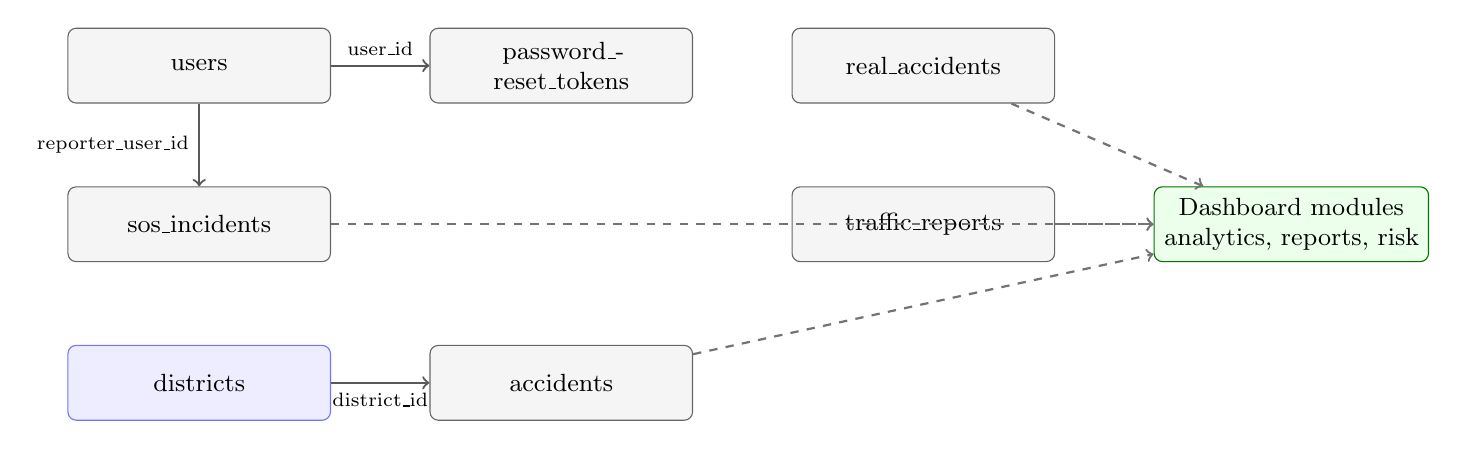
\begin{tikzpicture}[
  entity/.style={
    rectangle,
    draw=black!60,
    rounded corners=3pt,
    align=center,
    minimum height=0.95cm,
    text width=3.1cm,
    fill=gray!8,
    font=\small
  },
  module/.style={
    rectangle,
    draw=green!45!black,
    rounded corners=3pt,
    align=center,
    minimum height=0.95cm,
    text width=3.25cm,
    fill=green!8,
    font=\small
  },
  ref/.style={
    rectangle,
    draw=blue!55,
    rounded corners=3pt,
    align=center,
    minimum height=0.95cm,
    text width=3.1cm,
    fill=blue!7,
    font=\small
  },
  arrow/.style={->, thick, draw=black!65},
  dashedarrow/.style={->, thick, dashed, draw=black!55},
  node distance=1.05cm and 1.25cm
]

\node[entity] (users) {users};
\node[entity, right=of users] (tokens) {password\_reset\_tokens};
\node[entity, below=of users] (sos) {sos\_incidents};

\node[ref, below=of sos] (districts) {districts};
\node[entity, right=of districts] (accidents) {accidents};

\node[entity, right=of tokens] (real) {real\_accidents};
\node[entity, below=of real] (reports) {traffic\_reports};
\node[module, right=of reports] (dashboard) {Dashboard modules\\analytics, reports, risk};

\draw[arrow] (users) -- node[above, font=\scriptsize]{user\_id} (tokens);
\draw[arrow] (users) -- node[left, font=\scriptsize]{reporter\_user\_id} (sos);
\draw[arrow] (districts) -- node[below, font=\scriptsize]{district\_id} (accidents);
\draw[dashedarrow] (real) -- (dashboard);
\draw[dashedarrow] (reports) -- (dashboard);
\draw[dashedarrow] (sos) -- (dashboard);
\draw[dashedarrow] (accidents) -- (dashboard);

\end{tikzpicture}
}
\caption{Logical database model of AstanaSafe}
\label{fig:database_model}
\end{figure}

Some fields that might look similar are intentionally kept in different tables. For example, both \texttt{real\_accidents} and \texttt{traffic\_reports} contain coordinates, weather, and district values. However, the meaning of these fields is different. In \texttt{real\_accidents}, these values describe a historical accident. In \texttt{traffic\_reports}, they describe a submitted report of a current traffic situation. Keeping these tables separate makes it easier to show the source of information and avoid confusion between historical accident records and user reports.

\section{API Design and Backend Structure}

For AstanaSafe, the backend API was created using FastAPI. It serves as the middle layer between the React frontend and the PostgreSQL database that contains the system data. Frontend pages do not query the database directly, but send requests to the API endpoints of the corresponding backend modules. Each endpoint handles validation, authentication, database queries, business logic, and output serialization. This setup is appropriate because the dashboard has a wide variety of features, including analytical accident data, traffic reports contributed by users, SOS call handling, user management, risk analysis, AI-based forecasts, and RoadVision video processing.

The backend API is started in the main application file. The database models are connected to the database using SQLAlchemy. The database schema for the application is prepared, and compatibility updates for several fields are applied for the current project version. This concerns user roles, additional fields for traffic reports, and the \texttt{reporter\_user\_id} field for SOS incidents. After that, the FastAPI application is created. The application is called AstanaSafe API and has version 1.0. CORS configuration is also added because the frontend and backend can run on different local development ports. Localhost and LAN development addresses are allowed, while additional origins are passed from the environment.

In order to divide the backend system into separate areas, several routers were created. Each router manages its own part of the digital software system and keeps the backend environment cleaner. It is much easier to maintain this structure than a single large file where authentication, road data, accidents, traffic reports, risk analysis, SOS incidents, RoadVision, and AI forecast logic are placed together. The backend structure is also aligned with the frontend interface, even though the two layers work in different ways. The report form and Reports page use traffic report endpoints, My SOS and Dispatcher pages use SOS endpoints, and map forms and location selection use road endpoints. This keeps the system logic unified.

Most of the backend API follows a RESTful architecture. Data is requested with \texttt{GET}, created with \texttt{POST}, changed with \texttt{PUT} or \texttt{PATCH}, and deleted with \texttt{DELETE}. SOS calls are handled through a WebSocket endpoint because call events need to be exchanged in real time between driver and dispatcher while both are online. REST endpoints are more suitable for records, filters, reports, and status updates, while WebSocket communication is more suitable for a live call workflow.

The normal request flow starts from the frontend. A page or service on the frontend sends a request to the backend API. The route for this request is handled by the backend, and input data is validated. This can be done by a Pydantic schema or by the query parameters of a FastAPI endpoint. If authentication is required for this endpoint, the JWT token from the \texttt{Authorization} header is validated by the authentication dependency. After validation, the router either performs a direct query on the database or calls a service function. The result of this operation is returned to the frontend as JSON. Because all data has to pass through one server-side control layer before it is written to the database, the application stays predictable.

\begin{figure}[H]
\centering
\resizebox{\textwidth}{!}{%
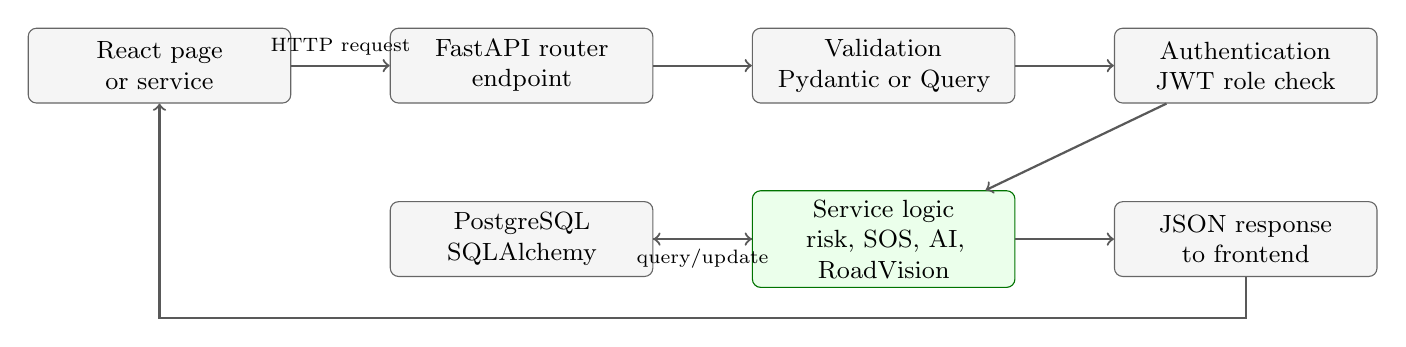
\begin{tikzpicture}[
  block/.style={
    rectangle,
    draw=black!60,
    rounded corners=3pt,
    align=center,
    minimum height=0.95cm,
    text width=3.1cm,
    fill=gray!8,
    font=\small
  },
  service/.style={
    rectangle,
    draw=green!45!black,
    rounded corners=3pt,
    align=center,
    minimum height=0.95cm,
    text width=3.1cm,
    fill=green!8,
    font=\small
  },
  arrow/.style={->, thick, draw=black!65},
  node distance=1.1cm and 1.25cm
]

\node[block] (frontend) {React page\\or service};
\node[block, right=of frontend] (router) {FastAPI router\\endpoint};
\node[block, right=of router] (validation) {Validation\\Pydantic or Query};
\node[block, right=of validation] (auth) {Authentication\\JWT role check};
\node[service, below=of validation] (logic) {Service logic\\risk, SOS, AI, RoadVision};
\node[block, left=of logic] (db) {PostgreSQL\\SQLAlchemy};
\node[block, right=of logic] (response) {JSON response\\to frontend};

\draw[arrow] (frontend) -- node[above, font=\scriptsize]{HTTP request} (router);
\draw[arrow] (router) -- (validation);
\draw[arrow] (validation) -- (auth);
\draw[arrow] (auth) -- (logic);
\draw[arrow] (logic) -- node[below, font=\scriptsize]{query/update} (db);
\draw[arrow] (db) -- (logic);
\draw[arrow] (logic) -- (response);
\draw[arrow] (response) -- ++(0,-1.0) -| (frontend);

\end{tikzpicture}
}
\caption{Backend API request processing flow}
\label{fig:api_request_flow}
\end{figure}

When a user registers or logs in, the server generates an access token, which is a JSON Web Token containing that user's identifier. The user includes that token in the \texttt{Authorization} header of later requests to endpoints that the user has access to. The server validates the token, looks up the user in the database, and then proceeds with the request. Failure to include a token, an invalid token, or a user identifier that does not correspond to an actual user results in an authentication error. This authentication is used for traffic report endpoints, profile endpoints, SOS incident endpoints, and administrator functions.

The system uses role-based access. Ordinary authenticated users can add traffic reports and SOS incidents. Dispatchers and administrators can update the status of SOS incidents, as this is part of the incident operational response workflow. Administrator-only access is granted to user management endpoints. In the backend, this is implemented through dependencies such as \texttt{get\_current\_user} and \texttt{require\_admin}. In SOS status update functionality, dispatcher access is also checked directly.

The backend is also responsible for password hashing and password reset tokens. Plain-text passwords are not stored in the backend. Passwords are hashed with the \texttt{bcrypt\_sha256} context. Password reset tokens are also hashed with SHA-256. The hashes of reset tokens are stored in the \texttt{password\_reset\_tokens} table. The backend checks token expiration and whether the token has already been used. Login with a Google account is also supported. The credential is verified against the client identifier configured for Google login.

The risk API provides an analytical engine. The \texttt{/api/risk/analyze} route processes data regarding latitude, longitude, radius in meters, and optionally a date. FastAPI validation ensures that both latitude and longitude values fall into valid coordinate ranges. The radius also has to fall within the system's defined acceptable range. Once the request is validated, the router invokes the \texttt{analyze\_zone} service function. This function finds nearby historical accidents and traffic reports, identifies contributing factors, and generates a structured risk assessment result. This allows risk assessment logic to stay outside the router file, making the analytical logic simpler to test \cite{xie2013}.

The SOS API provides the operational component of the platform. Users can create an SOS incident using the coordinates of where the incident occurred, road information, urgency level, a brief description of what happened, and reporter contact information. When a user submits an incident report, it is stored with the status \texttt{new} in the database, and a simulated notification log is generated for police, ambulance service, road service, and city dispatcher. Incidents can be filtered by active state or status. Dispatchers and administrators are able to change the status of an incident to \texttt{accepted}, \texttt{dispatched}, \texttt{resolved}, or \texttt{cancelled}. The WebSocket endpoint enables real-time communication between dispatcher and driver during call events such as call initiated, call accepted, call declined, call ended, WebRTC offer and answer, and ICE candidate messages.

\chapter{Practical Implementation of AstanaSafe}

\section{Implementation Environment and Project Structure}

The implementation of the diploma project relies on the AstanaSafe web application that was constructed as a practical software product. Developing AstanaSafe involved building a client-server structure where the frontend, backend, database, and prepared geospatial data exist as separate parts of the project. Keeping these parts distinct helps prevent confusion between interface code, server-side logic, stored data, and data preparation scripts. Because these parts remain separate, maintaining the implementation becomes simpler, and the diploma project becomes more understandable during a formal presentation.

The practical result goes beyond being a static interface. A working web dashboard is provided by the AstanaSafe web application, which can load documented road accident records, show safety indicators, and process user-submitted reports. Since the system also handles emergency-related scenarios, AstanaSafe supports SOS workflows for road users and dispatch-oriented users. The application also includes AI-assisted modules that help with data analysis and RoadVision video review. Each component of the system is supported by a clear project structure and by testing files used to check technical behavior.

The implementation environment was chosen in order to achieve the goals of the project. The system had to support an interactive map, analytical charts, user authentication, role-based functions, data storage, server-side validation, geospatial data processing, and possible future expansion. A modern JavaScript environment for the frontend is combined with a Python environment for the backend and a relational database. For the client side, React and Vite are used, while FastAPI is used for the server side. The data is stored in a PostgreSQL database. This environment is well suited for the diploma project because it allows fast development, clear separation of components, and flexible implementation of both analytical and operational modules \cite{chen2012}.

The frontend is constructed as a single-page application. It does not reload the entire page for each interaction. Instead, the browser loads the React application one time and then changes the displayed pages using routing. This is convenient for a dashboard where the user can move between Dashboard, Analytics, Reports, Danger Zones, District Passport, Forecast, My SOS, Dispatcher, RoadVision, Account, Settings, and Admin pages without interrupting the whole interface. Vite is used to build the frontend because it provides a fast local development server and a production build process. Page routing is implemented with React Router, and lazy loading is applied so that page components are loaded only when they are needed \cite{few2006}.

For building the backend, FastAPI was selected. FastAPI provides REST API endpoints and one WebSocket flow for handling SOS calls. It enables a clear router structure, validation with Pydantic schemas, automatic API documentation, dependency injection, and asynchronous handlers when they are required. SQLAlchemy is used for working with database models and making database queries. Alembic migrations are included to make sure the database schema is reproducible. Other backend responsibilities include authentication, password hashing, password reset functionality, role checking, traffic reporting, SOS incidents, risk analysis, RoadVision processing, and AI forecast support.

PostgreSQL is used as the central data management system for the project. It stores historical accident records, traffic reports from users, SOS incidents, user accounts, password reset tokens, and supporting entities. PostgreSQL is important because the system must not lose reports or user data when the browser session ends. A more realistic project structure is created when PostgreSQL is used instead of relying only on local browser state. Within the \texttt{real\_accidents} table, historical accident records gathered from the KPSSU/DTP dataset are kept, while the \texttt{traffic\_reports} table stores congestion and incident reports provided by users.

\renewcommand{\arraystretch}{1.2}
\begin{longtable}{|p{3.4cm}|p{4.7cm}|p{6.5cm}|}
\caption{\centering Technologies used in the implementation}
\label{tab:implementation_technologies} \\
\hline
\textbf{Technology} & \textbf{Use in the project} & \textbf{Main reason for selection} \\
\hline
\endfirsthead
\hline
\textbf{Technology} & \textbf{Use in the project} & \textbf{Main reason for selection} \\
\hline
\endhead
React & Frontend interface and page components & Builds a dynamic dashboard with reusable components. \\
\hline
Vite & Frontend development and production build & Provides fast local development and a simple build process. \\
\hline
React Router & Client-side navigation between dashboard pages & Allows users to move between different parts of the application without reloading the whole page. \\
\hline
Zustand & Frontend state management & Stores shared application state such as reports, filters, user data, map data, and modal states. \\
\hline
Leaflet and React-Leaflet & Interactive map & Displays map layers, markers, and location-based visualization on the web. \\
\hline
\texttt{leaflet.heat} & Heatmap-like accident visualization & Emphasizes dense areas of accidents. \\
\hline
Chart.js and \texttt{react-chartjs-2} & Analytical charts & Creates analytical charts to present accident and traffic report statistics. \\
\hline
Axios & Frontend API communication & Sends requests from the frontend to the FastAPI backend. \\
\hline
FastAPI & Backend API & Provides routers, validation, authentication dependencies, and API endpoints. \\
\hline
SQLAlchemy & Database models and queries & Maps backend models to the corresponding PostgreSQL tables. \\
\hline
PostgreSQL & Main database & Stores structured accident, report, SOS, and user data. \\
\hline
Alembic & Database migration control & Keeps database schema changes reproducible. \\
\hline
Pydantic & Request and response schemas & Validates API input and output data structures. \\
\hline
Pytest & Backend testing & Tests service functionality of the backend code. \\
\hline
\end{longtable}

The project directory is divided into frontend, backend, data, and documentation-related files. Inside the frontend folder, the React application and all page-level interface code are found. The backend folder holds the FastAPI application, routers, models, schemas, services, migrations, scripts, data files, and tests. The data folder contains larger source data files used to prepare road and district information. Because this organization is established, mixing interface code with backend logic and data preparation scripts is avoided.

Pages in the frontend are organized according to how users interact with the software. Analytical pages include information related to road accidents, traffic congestion, district-specific reports, and dangerous zones. Operational pages are used to manage SOS calls received from drivers, dispatcher actions, and response scenarios. Account-related pages provide access to user identity functions, authentication state, settings, and administrator tools. This structure makes it easier for each user group to navigate the system and reflects the role-based logic discussed in the previous chapter.

The backend modules follow the same organization. Authentication logic is located in the authentication router. Traffic report logic is placed in the traffic reports router. Historical accident data is exposed through the real accidents router. Road and district data are served through the roads router. Risk analysis is segmented into two components: the risk router and the risk analysis service. SOS incident creation, status updates, and WebSocket call signaling are grouped in the SOS router. RoadVision functionality is placed in its own router because video processing has a different request pattern from regular JSON endpoints. AI forecast and dashboard insight functions are separated into their own router and service layer.

Services are essential because all backend logic cannot be placed inside API route functions. Route functions should receive input, validate access, and provide a response, while more complex calculations and processing should be placed in service modules. In AstanaSafe, this is done for risk analysis, AI forecast generation, RoadVision analysis, and email sending. For instance, the risk analysis router receives coordinates and a radius, but the real calculation happens within the risk analysis service. This means that the code is easier to test and route files do not become too large.

Specific geospatial files are incorporated into the technical setup and prepared in advance. Records were extracted from the original \texttt{DTP.geojson} file so that historical accident data for Astana could be kept in the \texttt{astana\_dtp.geojson} document. Information regarding roads and intersections is maintained in the \texttt{astana\_streets.json} and \texttt{astana\_intersections.json} formats. Boundaries for specific districts are located within the \texttt{astana\_districts.geojson} resource. These geospatial files allow the backend and frontend to display map context, road selection, district layers, and risk analysis. Because the system values efficiency, the geospatial files are not retrieved from an external source every time the dashboard is opened. The files are processed in advance, and then the application serves the prepared data directly to the user.

To prepare and maintain this project, several scripts are used. Correctness of information is supported when the extraction script filters accident records for Astana. Through the import script, the prepared accident records are deposited into the \texttt{real\_accidents} database table. Changes regarding the database schema are executed by migration scripts. Bootstrap and database checking scripts give assistance when the system is prepared for local execution. This script-based workflow is useful because the project can be recreated without difficulty. If the database contains no information, the prepared dataset can be loaded again using the same import logic.

The application was also prepared for local development and demonstration. The project provides startup scripts for Windows and macOS. These scripts install the necessary dependencies, structure the backend environment, process database migration logic, and start backend and frontend servers. Uvicorn uses port 8000 to run the backend during manual operation, while Vite runs the frontend on port 5173. Since a configured API base URL is present, the connection between the frontend and backend is achieved through the same API structure used by the implemented pages.

During development, verification of technical components was performed because automatic backend tests analyze AI forecast logic, password recovery behavior, geospatial risk evaluation helpers, and RoadVision data processing. These tests check not only that the software product starts correctly, but also that crucial backend services operate according to their design. The frontend is verified through the production build process. A successful build shows that the React application can be compiled into files suitable for deployment.

To represent the main objective of this diploma project, the AstanaSafe implementation architecture is used as a practical foundation. The implementation is wider than a single picture or one visualization because it contains an operator dashboard, server-side communication methods, structured information repositories, geospatial preprocessing, evaluation records, different user rights, emergency assistance workflows, and additional AI-assisted modules. By using this framework, the concrete implementation is connected to an active urban decision support system, which establishes a foundation for the detailed discussion of interface elements in the following sections.

\section{Dashboard and Interactive Map Implementation}

The AstanaSafe Dashboard is the main working screen of the application. It was intentionally designed as the first interface that the user sees in order to reduce the need to use several different tools to understand the road safety situation in Astana. Instead, the user receives a quick overview of the road safety state in the city and can then continue with more detailed analysis through other modules of the application.

Within this interface, the essential information about road safety in Astana is presented. This includes summary indicators, an interactive city map, filtering options, recent activity data, district report data, weather data, and AI-assisted safety forecast data. The implemented Dashboard page is shown in Figure~\ref{fig:dashboard_main_page}.

\begin{figure}[H]
\centering
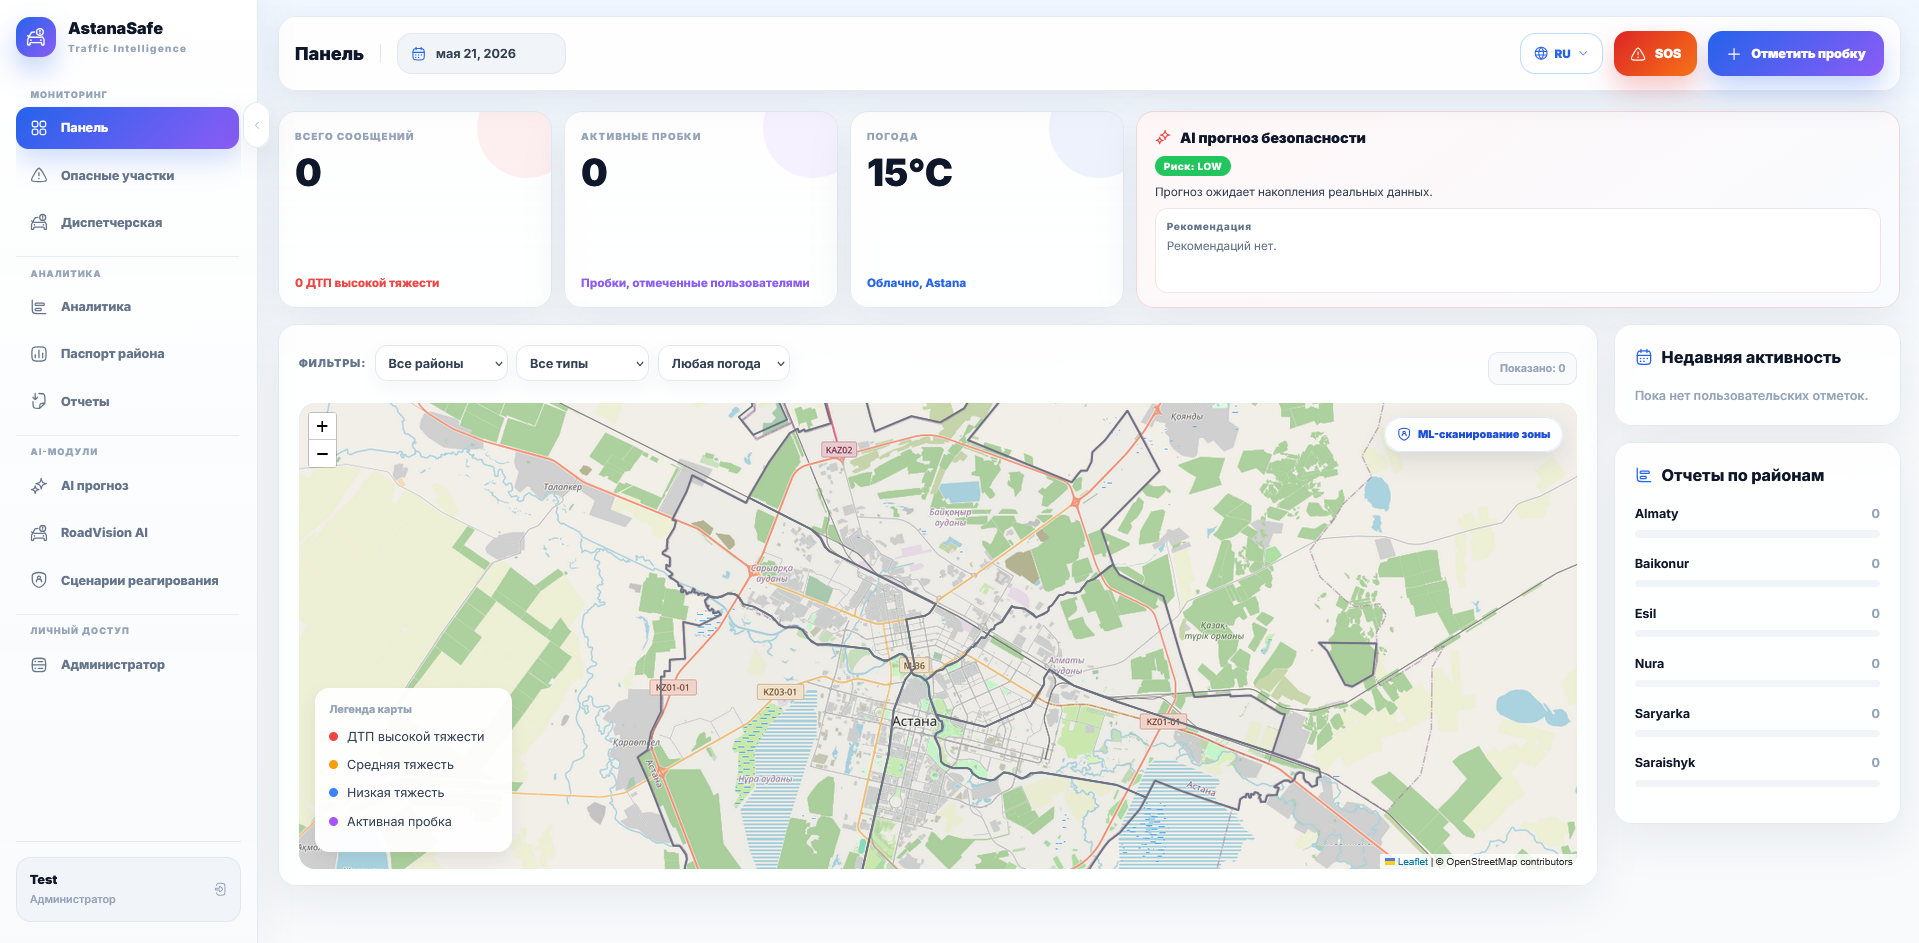
\includegraphics[width=\textwidth]{figures/dashboard_main_page.png}
\caption{Main Dashboard page with summary indicators and interactive map}
\label{fig:dashboard_main_page}
\end{figure}

As shown in Figure~\ref{fig:dashboard_main_page}, the Dashboard combines analytical indicators, map-based accident visualization, filtering controls, and recent user activity in one working interface. This layout supports the main purpose of AstanaSafe because it gives the user both a general overview and access to more detailed road safety information.

The Dashboard is represented by the React file \texttt{Dashboard.jsx}. Rather than creating the dashboard as a single visual component, several smaller components were created and then combined into one page. These include \texttt{Topbar}, \texttt{StatCard}, \texttt{SectionCard}, \texttt{FilterPanel}, \texttt{AccidentMap}, and smaller components for the map legend, recent activity, district report rows, and AI forecast card. Each of these components has a specific role within the application and inside the Dashboard page.

Primary data is delivered to the Dashboard through the custom hook \texttt{useDashboardData}. This hook collects accident records, traffic reports, selected date, filters, weather information, current user state, and AI forecast information from the Zustand application store and backend services. When the Dashboard is opened, \texttt{useDashboardData} requests accidents, heatmap data, weather, traffic reports, and forecast information. The collected information is then arranged and prepared for presentation to the user. Historical accident records and user-submitted traffic reports are converted into a common display format so that they can appear together on the map and be processed using the same dashboard indicators.

The indicators at the top of the Dashboard provide an overview of the selected situation. The first card displays the total number of reports for the selected date and filters. In the subtitle of this card, the number of high-severity accident records is displayed. The second card displays the number of active traffic jams. The third card displays weather information obtained through the application store. The fourth card is an AI safety forecast card that displays information about the safety of the selected date and area. The card uses AI forecast logic from the backend of the application. If the AI model is unavailable, fallback data is used to populate the card. This ensures that the card is visible and functional even during demonstration of the application \cite{vlahogianni2014}.

The Dashboard does not display all accident records at the same time. The application store contains filters for district, accident type, and weather. After accident and traffic report records are normalized, the Dashboard applies the selected filters from the application store. For example, if a particular district is selected with the filter, only accident and report records from that specific district remain visible on the screen. The same logic is applied to the other filters. This makes the Dashboard more analytical because the user can compare specific conditions rather than reading the entire dataset at the same time.

The interactive map is created using the Leaflet and React-Leaflet libraries in the \texttt{AccidentMap} component. The map is centered on the city of Astana and uses OpenStreetMap tiles \cite{leafletDocs}. On top of that layer, district boundaries are shown with a GeoJSON overlay using prepared data for each district. Traffic reports and accident records are presented as circle markers on the map. Every marker has a different color according to the class of the record. Red represents severe crashes, orange represents moderate crashes, blue represents minor crashes, and purple is used to indicate active traffic jams. This color coding enables users to identify types of accidents or traffic jams without opening report tables.

Each marker also includes a popup that shows information about the selected traffic report or accident record. The popup shows the classification of the record, road or accident location description, district, accident type, and weather conditions. This information is shown in a clear format so that the user can quickly see what kind of accident or traffic situation has been recorded without opening a full table. Users can select points of interest on the map and view detailed information about specific records. The map can also automatically focus on a recently created report point. After a new traffic report is submitted, the Dashboard can focus on this map and fly to the location of the newly created report.

A separate interaction is implemented for risk analysis. By clicking on an empty point of the map, the coordinates of this point are stored as a risk point. A request is sent to the backend risk analysis endpoint, including latitude, longitude, radius of the analysis, and optional date. In the current map implementation, the default radius is 450 meters. The response from the backend includes information about risk at the selected point, the number of related accidents and traffic reports, reasons for the risk score, possible interventions to reduce the risk, and the polygon of the analyzed zone. This information is displayed in the \texttt{RiskAnalysisPanel} and visualized on the map as the analyzed zone polygon. As a result, the map becomes an interactive tool for traffic risk analysis.

Traffic reporting is connected to the Dashboard through the Mark traffic action. If the user is not authenticated, the authentication modal is opened first. Otherwise, the \texttt{TrafficJamModal} is opened. There are two ways to create a traffic report. In the standard mode, the user chooses the road and crossroad using prepared road data. In the map-point mode, the report is connected to the point chosen on the map. The coordinates are sent to the backend, which finds the nearest road location. The report form asks for category, type, weather conditions, duration of the traffic jam, traffic flow, number of blocked lanes, and notes. The implemented traffic report modal is shown in Figure~\ref{fig:traffic_report_modal}.

\begin{figure}[H]
\centering
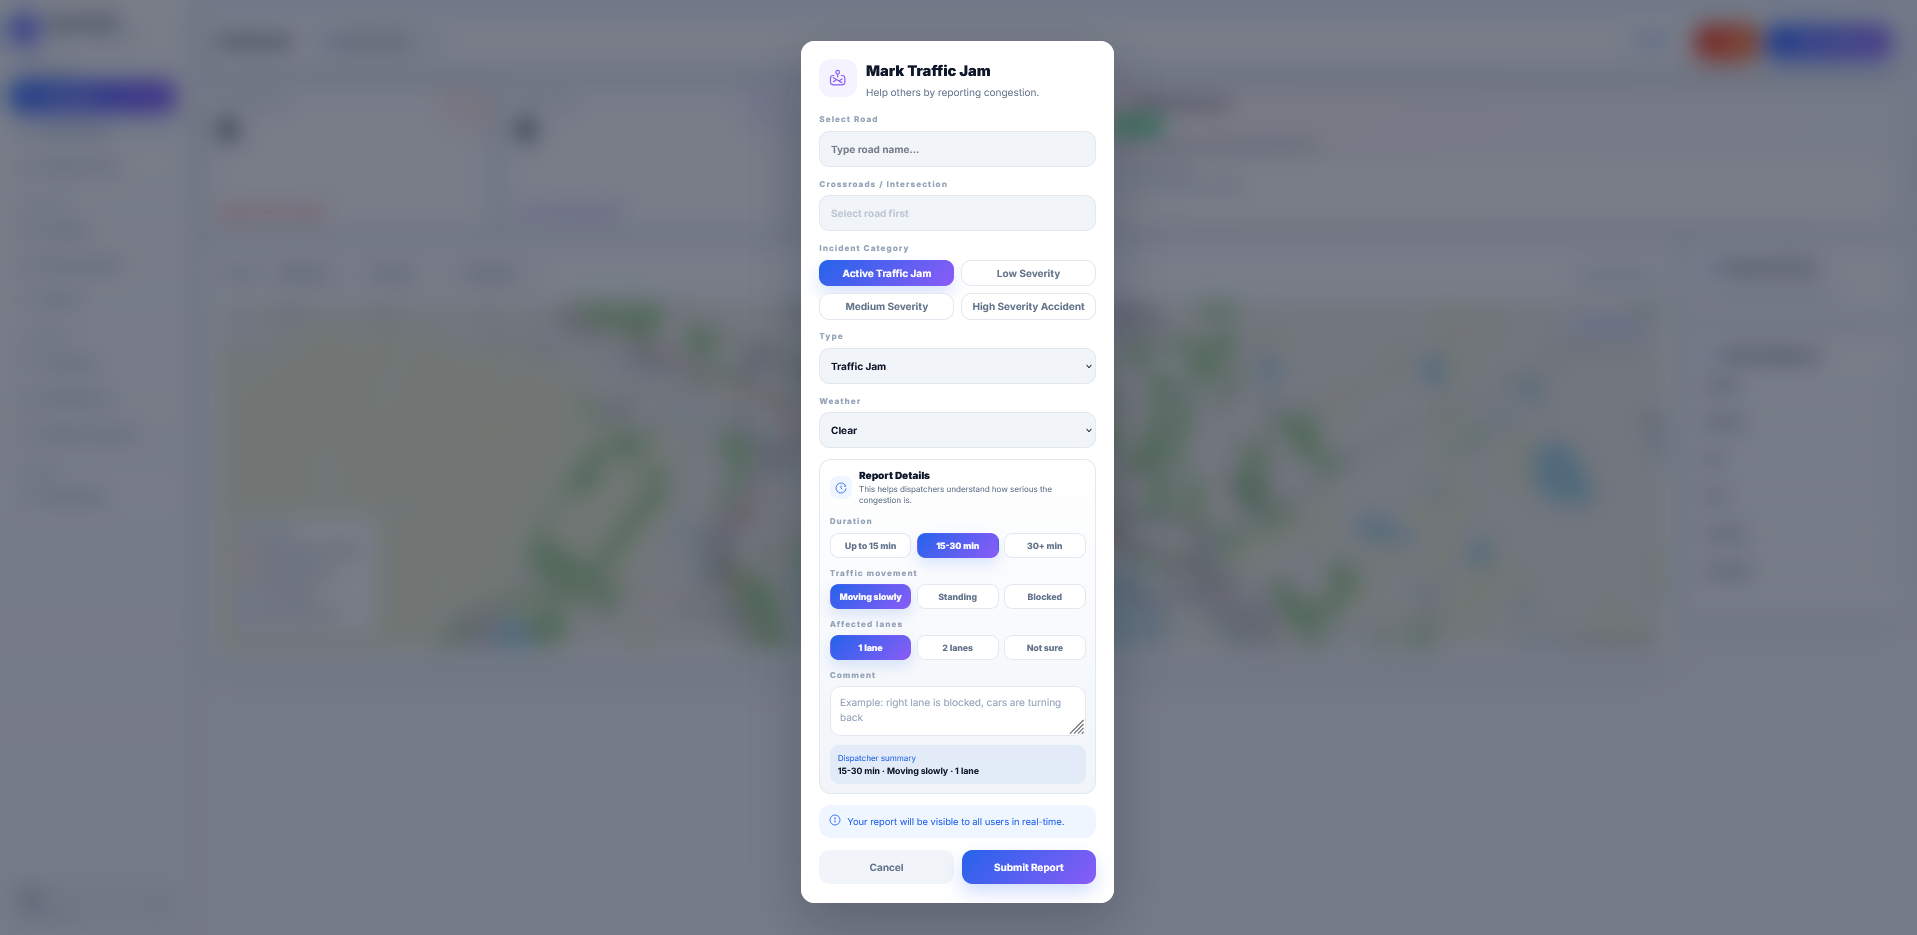
\includegraphics[width=\textwidth]{figures/traffic_report_modal.png}
\caption{Traffic report modal for submitting congestion and incident reports}
\label{fig:traffic_report_modal}
\end{figure}

Figure~\ref{fig:traffic_report_modal} shows that the report form stores not only coordinates, but also contextual attributes that are later used in dashboard visualization, report tables, and risk analysis. After the report is submitted, it is stored in the backend and becomes available on the Dashboard map, activity list, Reports page, and risk analysis module.

The recent activity panel displays the latest user-submitted reports. Only a few records are displayed on the Dashboard at one time in order to keep the interface compact. When additional activity logs are available, the user can open the complete activity log modal. This modal includes a search function, tabs for all records, accident log records, and traffic log records. It also includes small counters showing the total number of logs, recent hour logs, accidents, and traffic jams. This function is useful because it allows the map-based overview to be linked with a detailed list of recent user activity.

The district report block compares the number of visible records within each district of Astana. Currently, the implementation uses the following districts: Almaty, Baikonur, Esil, Nura, Saryarka, and Saraishyk. Each district has a horizontal bar within the district data visualization block. The width of the bars is compared to the district that has the maximum number of records. This makes it easy for the user to understand which district currently has the most records according to the selected filters and date.

The Dashboard also serves as a navigational bridge to the other modules within the platform. The map and indicators offer users the first overview of the platform. The Reports page offers a more detailed view of data in tables. The Analytics page offers deeper analysis of the data in the form of charts. The Danger Zones page allows users to focus on the most dangerous areas of the city. The District Passport page allows users to obtain an overview of each district. There are also pages dedicated to SOS and dispatcher work. For this reason, the Dashboard is not a standalone page. It is the central page that connects the analytical and operational aspects of AstanaSafe.

The implementation of the Dashboard demonstrates the main practical contribution of the project. Information gathered from accident records, traffic reports from users, weather data, district information, road information, filters, and AI forecast results is displayed on one screen so that the user can understand the road situation in Astana, inspect map points, create a traffic report, compare districts, and request accident risk analysis for the selected map location. This means that the Dashboard contributes to the project as a practical screen that displays information necessary for analyzing road safety in the city of Astana.

\section{Analytics, Reports and Data Visualization}

The Analytics and Reports pages extend the functionality of the Dashboard page. The Dashboard provides users with an overview of the most important data, while Analytics and Reports allow the data to be inspected in more detail. Two types of data are used in these pages: traffic accident records imported from external sources and traffic reports submitted by users of the application.

The Analytics page, implemented in the \texttt{Analytics.jsx} file, uses the Chart.js library through the \texttt{react-chartjs-2} package. This page loads traffic reports submitted by users and accident records from the backend accident history. Both types of records are normalized before being displayed on the page. Since traffic reports and accident records have different fields and origins, helper functions transform the data from both sources into common categories that can be displayed in charts and metric cards.

The upper section of the Analytics page contains metric cards that provide a brief description of the selected day. The total number of incidents shows the combined amount of historical accident records and user reports. The high severity ratio displays the share of records grouped as high severity. The peak incident hour identifies the hour when the largest number of records is observed by the system. The safe districts indicator evaluates districts with a small number of daily records. These values are not stored as separate database fields because the frontend calculates them from the records loaded for the selected date.

The central part of the Analytics page contains several charts. The hourly distribution chart explains how incidents are distributed throughout the day. The incident type chart shows the share of collisions, pedestrian-related events, rollovers, traffic jams, and other event categories. The severity by district chart compares low, medium, and high severity records across districts. District records present the number of records in every district. The congested arteries chart ranks roads with the greatest number of user reports. The weather impact chart links incidents with weather categories. Together, these charts transform raw records into readable analytical patterns \cite{wilkinson2005}.

The implemented Analytics page is shown in Figure~\ref{fig:analytics_page}.

\begin{figure}[H]
\centering
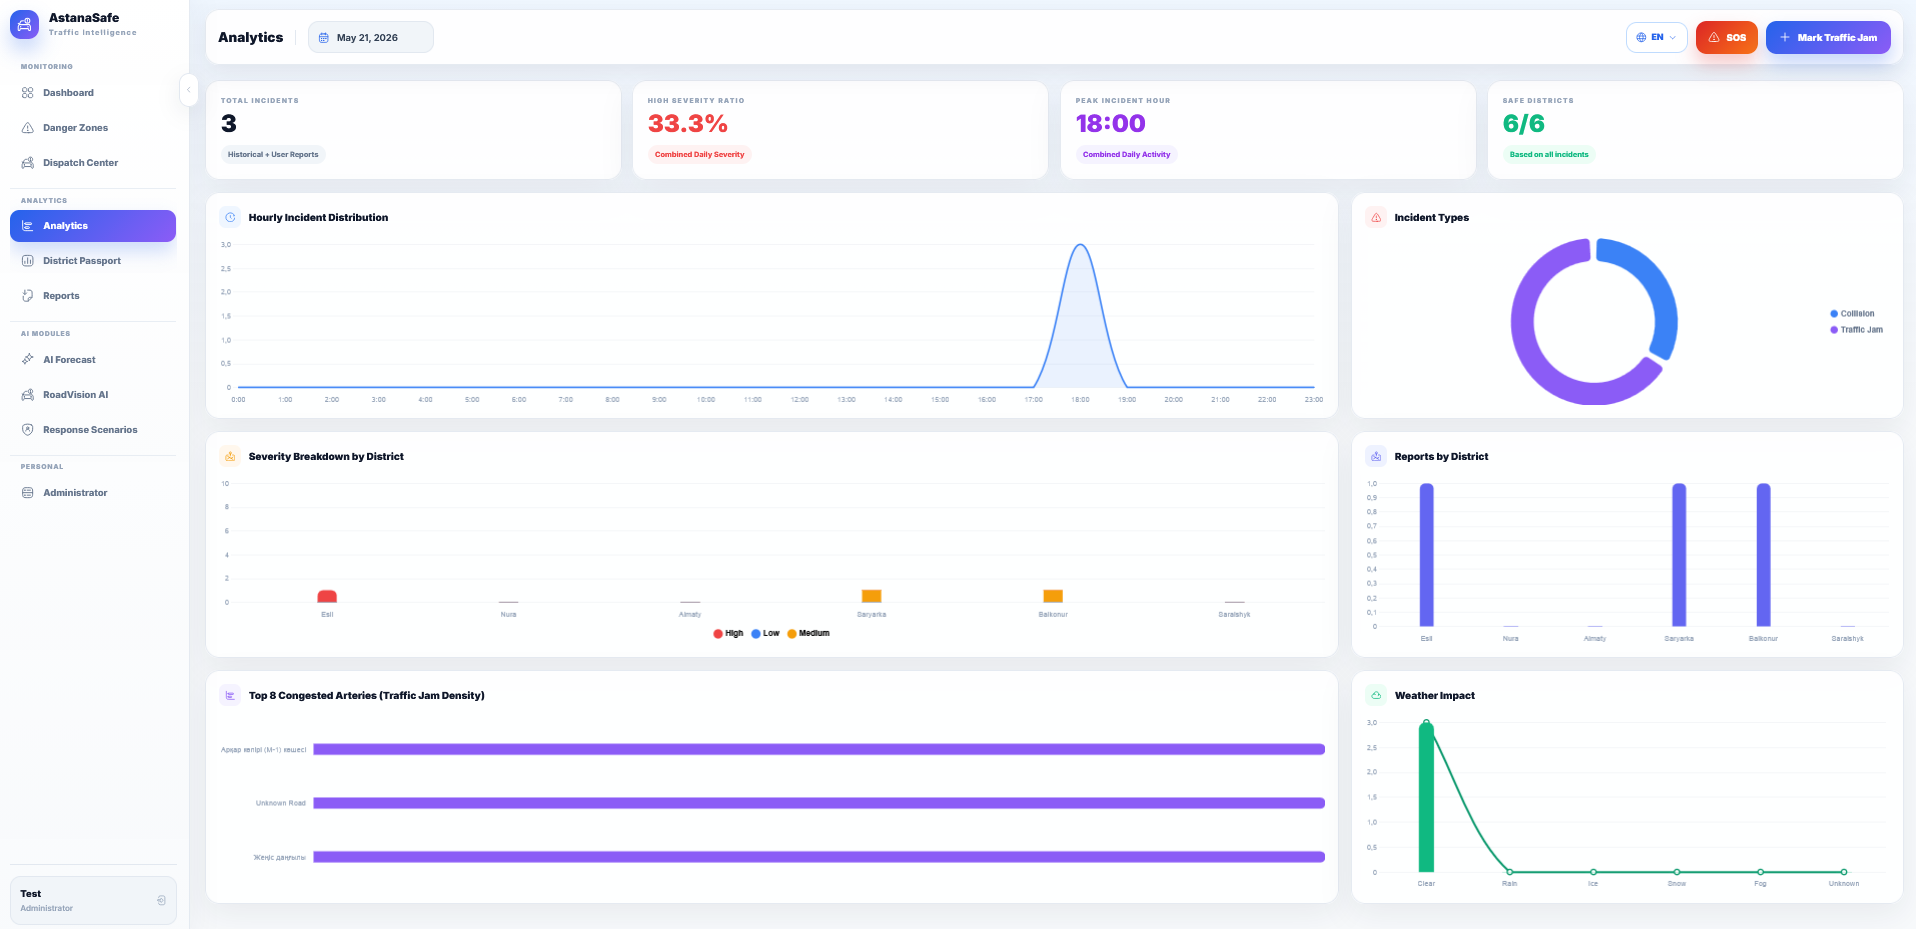
\includegraphics[width=\textwidth]{figures/analytics_page.png}
\caption{Analytics page with road safety indicators and charts}
\label{fig:analytics_page}
\end{figure}

Figure~\ref{fig:analytics_page} shows that the Analytics page is focused on visual comparison. The page combines daily indicators with several chart types, which helps to identify time patterns, district differences, dominant incident categories, and the influence of weather conditions.

The Reports page is implemented in the \texttt{Reports.jsx} file and focuses on table-based data inspection. Historical accident records and user-submitted traffic reports are loaded, transformed into similar report rows, and arranged according to their dates. The page displays three main indicators: the total number of filtered reports, the high severity rate, and the most active area. When the selected date range is modified, these indicators are recalculated by the system.

In addition to displaying the total number of incident reports, the Reports page includes date filtering and direct navigation to selected records. If a custom date range has not been selected, the table uses the global date from the application store. If a start date or an end date is chosen, the table is filtered by that interval. Each row shows date and time, district, type, severity, weather, and an action button. The action button sends the selected point back to the Dashboard map, sets the date, and focuses the map on the selected record. This connects table-based analysis with map-based analysis. The implemented Reports page is shown in Figure~\ref{fig:reports_page}.

\begin{figure}[H]
\centering
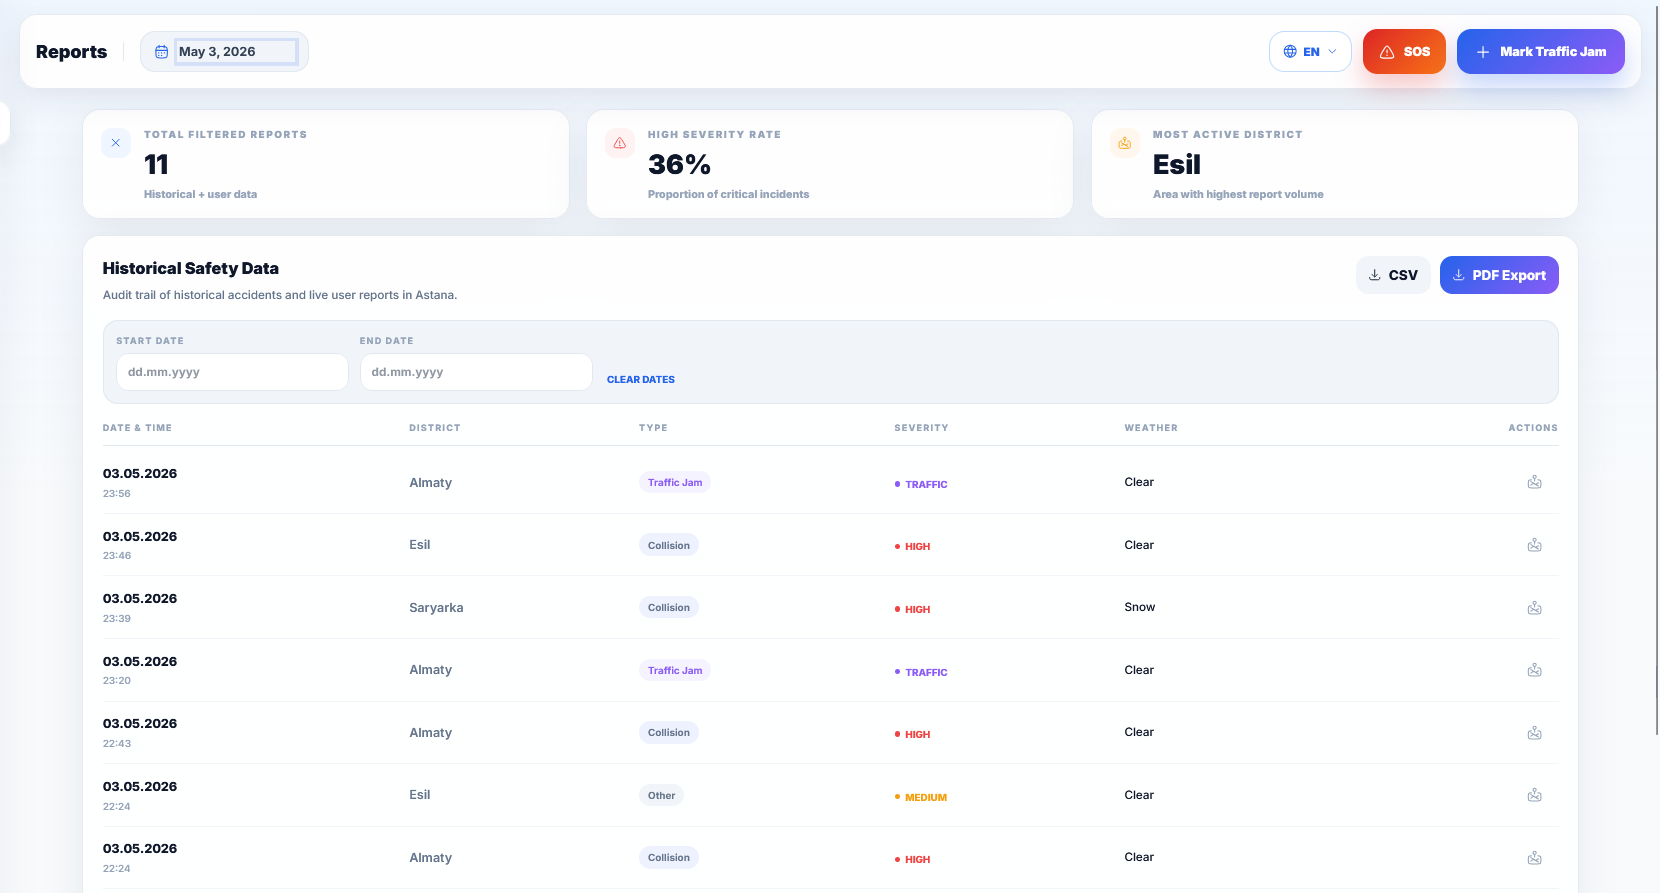
\includegraphics[width=\textwidth]{figures/reports_page.png}
\caption{Reports page with date filtering and structured incident table}
\label{fig:reports_page}
\end{figure}

As shown in Figure~\ref{fig:reports_page}, historical accidents and traffic reports are listed together in one table. Accident types, severities, weather conditions, coordinates, and districts are normalized in historical records. Traffic reports are standardized according to category, report type, weather, coordinates, creation date, and time. The interface uses badges and color indicators to simplify scanning of the table. For example, severe records are marked differently from mild records, and traffic jams have a distinct visual presentation separate from ordinary accident types.

The Reports page also contains buttons for exporting reports in CSV or PDF format. Although export is not the main focus of the diploma project, this function is important because the system should not only display data to users, but should also allow the data to be used in additional reports or research work.

The implementation of Analytics and Reports indicates that AstanaSafe is not only a map application for the city. It also provides data analysis through charts, tables, filters, color indicators, and export functions. These pages support the main goal of the project because they make accident and traffic information usable for detailed inspection and further research.

\section{Danger Zones and District Passport}

The Danger Zones and District Passport pages expand the analytical part of the application. On the Dashboard, users can see individual points and reports. On these pages, the same data is grouped according to the most risky locations in the city or according to the districts that comprise Astana.

The Danger Zones page was implemented in the \texttt{DangerZones.jsx} file. This page loads accident records and traffic reports from the backend. These data are further processed in the \texttt{buildDangerZones} function in the \texttt{cityInsights.js} file. The function takes both accident and traffic data and normalizes them to account for the fact that the two data sources have different structures. After normalization, the data are grouped either according to road name and district if they originate from traffic reports or according to coordinate buckets if they originate from accident records. For each danger zone, the system counts the number of accident records, traffic reports, high-severity cases, and hourly activity records.

These zones are then provided with a risk score based on accident records, traffic reports, and the number of high-severity cases in those zones. The more accidents, traffic reports, or high-severity cases are present in a zone, the higher its risk score. The zones are sorted according to their risk scores, and the system displays the top ten zones to the user. Each zone is also provided with a risk level of medium, high, or critical. Hazardous location identification depends on clear and operational risk definitions \cite{elvik2008}. Such an explanation of the construction of the risk scores is suitable for this diploma project, as the outcome of the project can be explained to the user and does not depend on a black-box prediction model \cite{lord2010}.

The interface of the Danger Zones page includes three main components: summary metrics, an interactive map, and a ranked list. The map displays Leaflet markers that indicate the risk level and accident records within each zone. When a zone is selected on the map, a popup displays the district that contains that zone, accident records for that zone, and traffic reports for that zone. The ranked list provides the same information as the map displays, but in a table-like format that allows users to compare different zones without referencing the map. The implemented Danger Zones page is shown in Figure~\ref{fig:danger_zones_page}.

\begin{figure}[H]
\centering
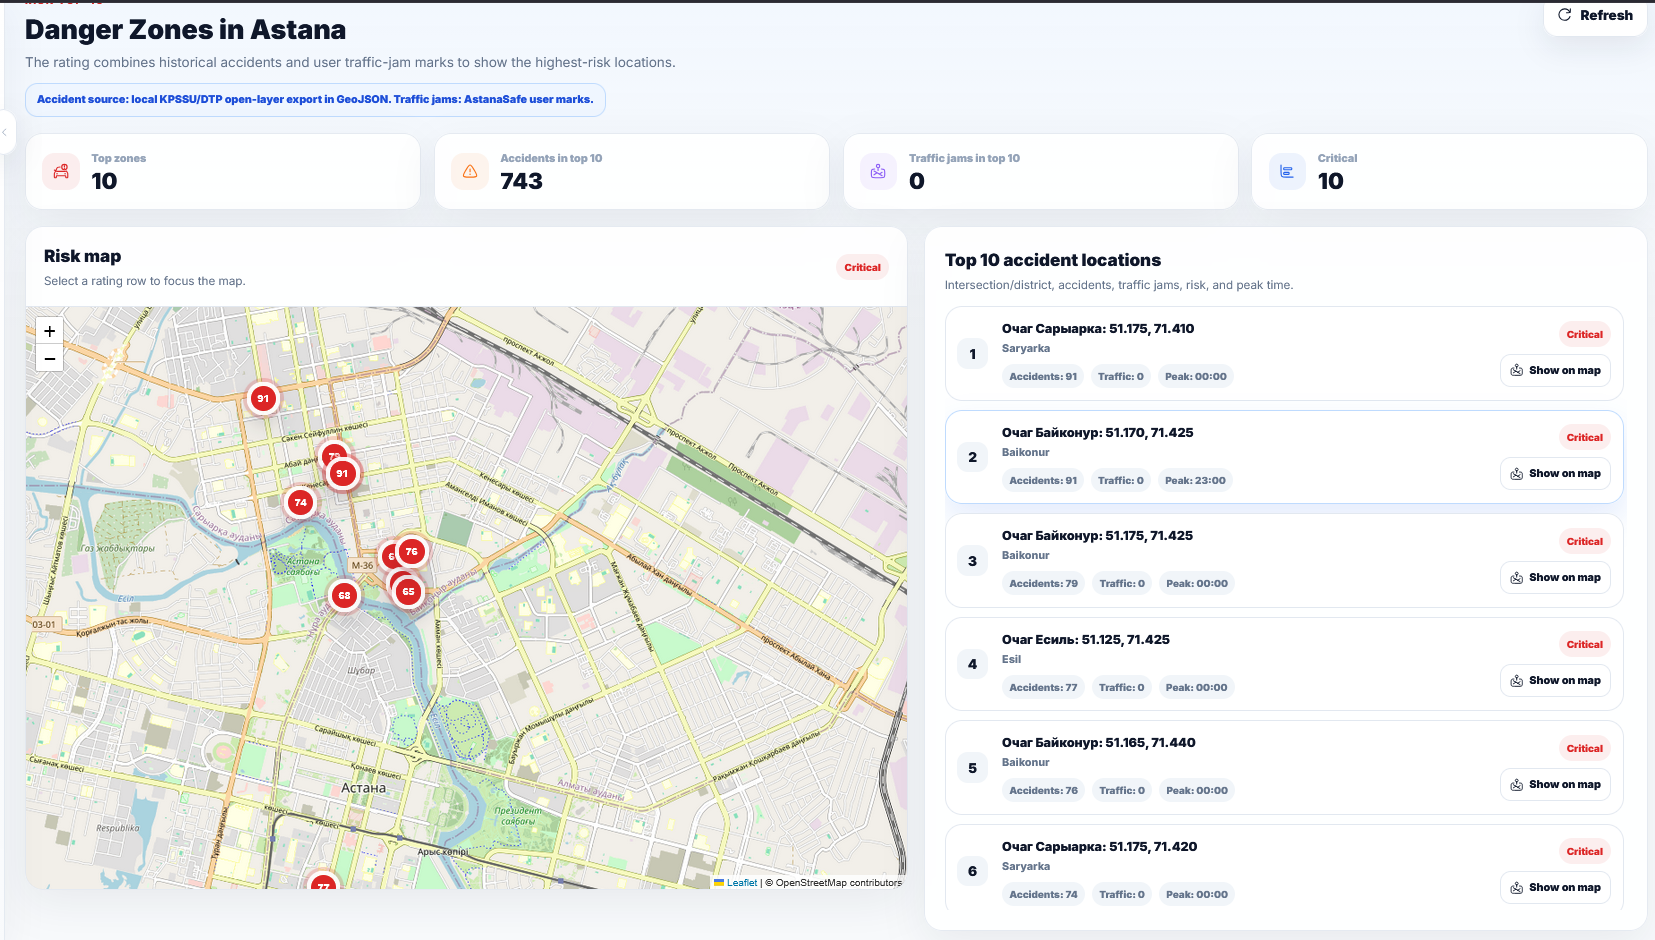
\includegraphics[width=\textwidth]{figures/danger_zones_page.png}
\caption{Danger Zones page with ranked risk zones and interactive map}
\label{fig:danger_zones_page}
\end{figure}

The District Passport page for comparing road safety indicators within a single district is implemented in \texttt{DistrictPassport.jsx}. The page loads the same two data sources: historical accident data and traffic reports submitted by users. The \texttt{buildDistrictPassport} function filters the records for the selected district and selected year, then computes the same set of district indicators: the number of accident records, the number of traffic reports, the total number of events, high-severity cases, the peak hour, the most active roads, and weather factors.

There is a year filter because road safety indicators change over time. Without it, a district with many old accidents could get higher passport indicators than a district with fewer accidents but more recent ones. The activity chart displays incident distribution by hour of day, allowing district indicators to be evaluated even when the district has only a moderate number of incidents with a clear peak during the hours when the city is most active \cite{andrienko2013}. Spatio-temporal analysis is important because urban mobility data changes by location and by time \cite{atluri2018}.

The implemented District Passport page is shown in Figure~\ref{fig:district_passport_page}.

\begin{figure}[H]
\centering
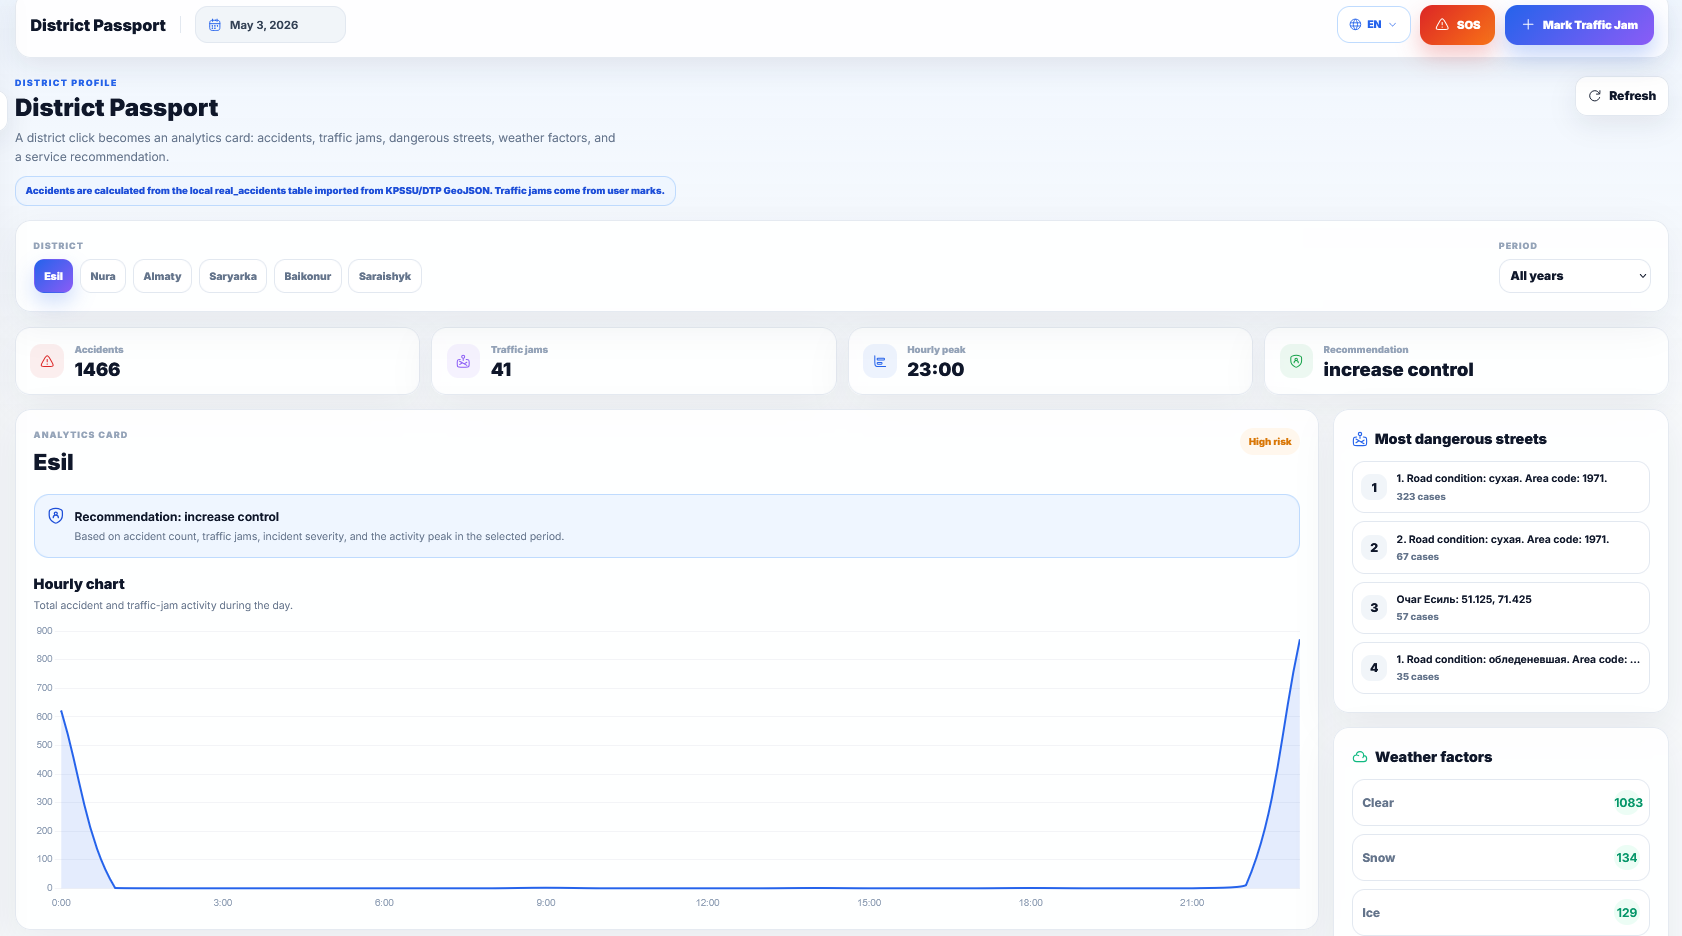
\includegraphics[width=\textwidth]{figures/district_passport_page.png}
\caption{District Passport page with district indicators and hourly activity chart}
\label{fig:district_passport_page}
\end{figure}

Recommendations on the District Passport page are generated from local indicators. If there are many high-severity cases or a large number of total cases in a district, stronger control is recommended. If traffic incidents are predominant and make up the bulk of accident records, then checking the organization of traffic light signals is recommended. In other cases, installing warning signs is sufficient as a basic safety measure. These recommendations are not treated as official engineering design, but rather as guidelines that can be used as prompts for interpreting dashboard data and possible actions.

These two pages support the main objective of AstanaSafe, as it not only stores data related to road accidents and congestion, but also groups them into views suitable for analysis. In Danger Zones, hot spots where problems regularly occur can be easily identified, while in District Passport, summary statistics for each district can be viewed. This makes AstanaSafe a suitable tool for researchers, students, analysts and city-oriented users who need to see not only where accidents occur, but also how they are distributed over roads, districts and time.

\section{SOS, Dispatcher Panel and Response Scenarios}

The SOS, Dispatcher and Response Scenarios modules represent the operational part of AstanaSafe. Although the Dashboard, Reports and Analytics pages are mostly used for analyzing accident and traffic data, the SOS workflow demonstrates that the same platform can support a practical response process. The emergency service dashboard is not intended to replace an official emergency service platform. However, it shows how a road safety dashboard can be extended from analysis to incident coordination.

An SOS event is created when an authenticated user opens the emergency modal from the interface. The form includes geographic information, road and crossroad information, district, urgency level, description of the reported problem, and contact details of the reporter. Once the form is submitted, the frontend passes the data to the backend using the SOS API. The backend validates the request, stores the incident in the \texttt{sos\_incidents} table and assigns the initial status \texttt{new}. The saved event includes date and time stamps, along with a notification log that imitates services such as police, ambulance, road service and city dispatcher being notified.

The \texttt{My SOS} page shows SOS reports and their current status. This is helpful because the user can see whether the signal was created and how it is being processed. For each incident, the page displays date, location, progress stages and a small map. The progress stages follow the same operational logic as the backend statuses: created, accepted, service dispatched and resolved.

The Dispatcher page is the main working screen for dispatch-oriented users. This page loads SOS incidents from the backend and displays them as map markers and incident cards. It also shows summary metrics for new, dispatched and resolved signals. For each incident, the dispatcher can view location coordinates, district, road, urgency level and reporter information. The dispatcher can change the status of the incident from \texttt{new} to \texttt{accepted}, from \texttt{accepted} to \texttt{dispatched}, and from \texttt{dispatched} to \texttt{resolved}. The backend protects this operation with role checking, so ordinary users cannot update dispatcher statuses.

The module also includes a call flow that is connected with SOS handling. The backend has a WebSocket endpoint for signaling, while the frontend handles call states such as ringing, connecting and active call. This makes the scenario more realistic because the incident is not treated only as a static record. The system can model communication between the driver and the dispatcher while the incident is being processed.

The Response Scenarios page presents the SOS process as a sequence of response stages. It shows the selected incident, its current status and the stage that corresponds to this status. These stages include the driver sending a signal, dispatcher acceptance, police notification, service dispatch and incident completion. The status and notification log make it clear which part of the response is already completed and which part remains active. This makes the workflow easier to understand during demonstration.

The implemented dispatcher and response scenario interfaces are shown in Figure~\ref{fig:sos_operational_pages}.

\begin{figure}[H]
\centering
\begin{subfigure}{0.49\textwidth}
\centering
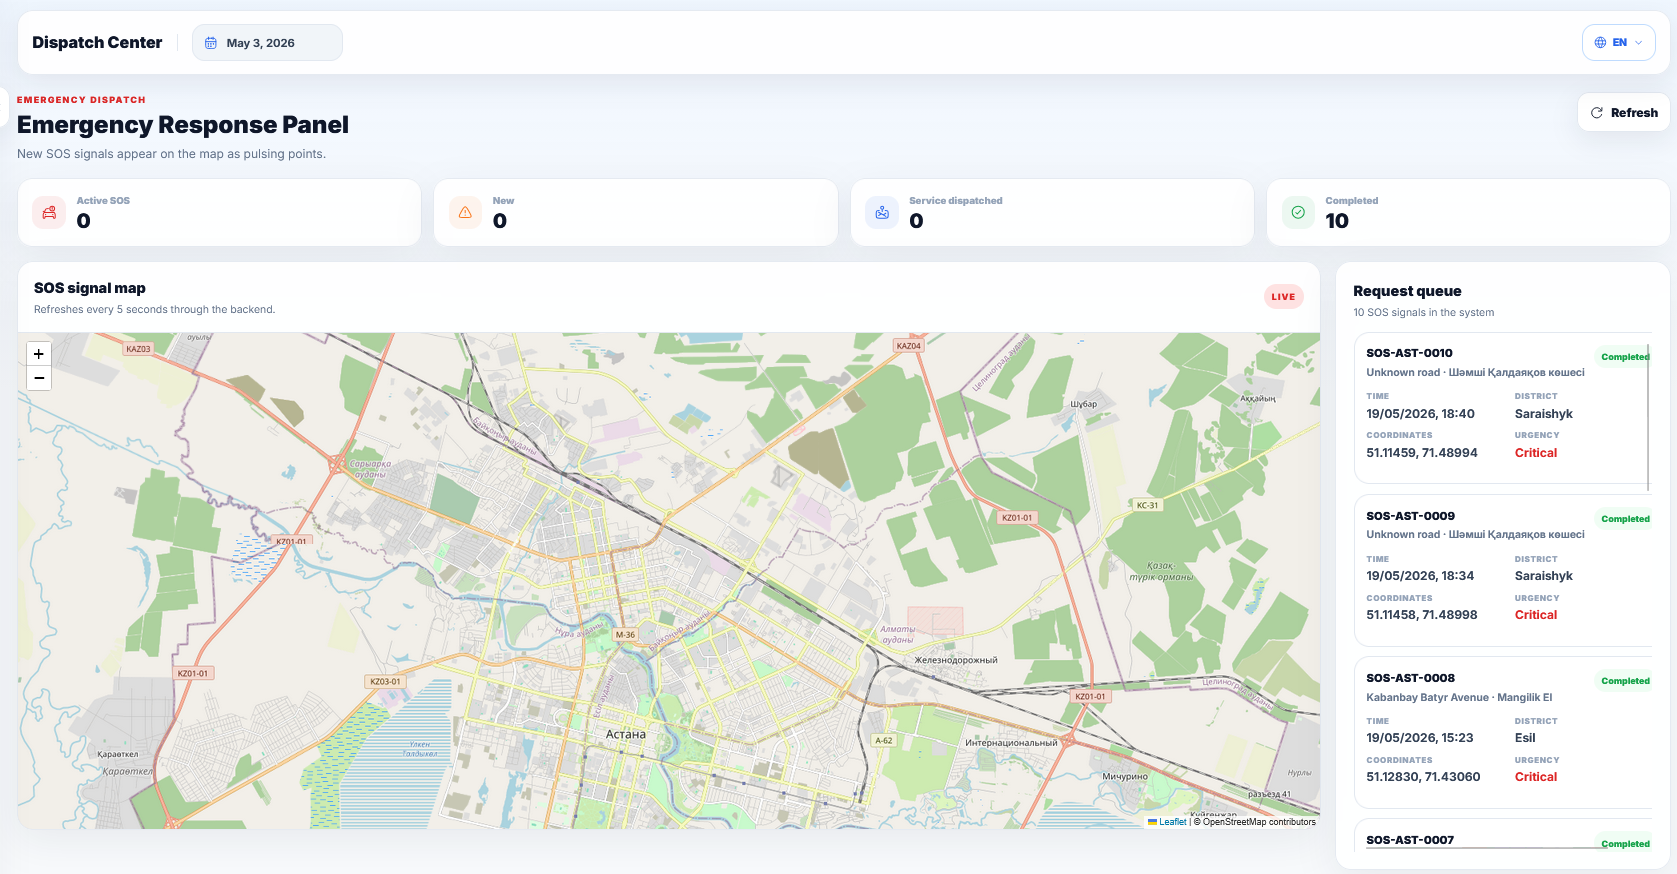
\includegraphics[width=\textwidth]{figures/dispatcher_page.png}
\caption{Dispatcher panel}
\end{subfigure}
\hfill
\begin{subfigure}{0.49\textwidth}
\centering
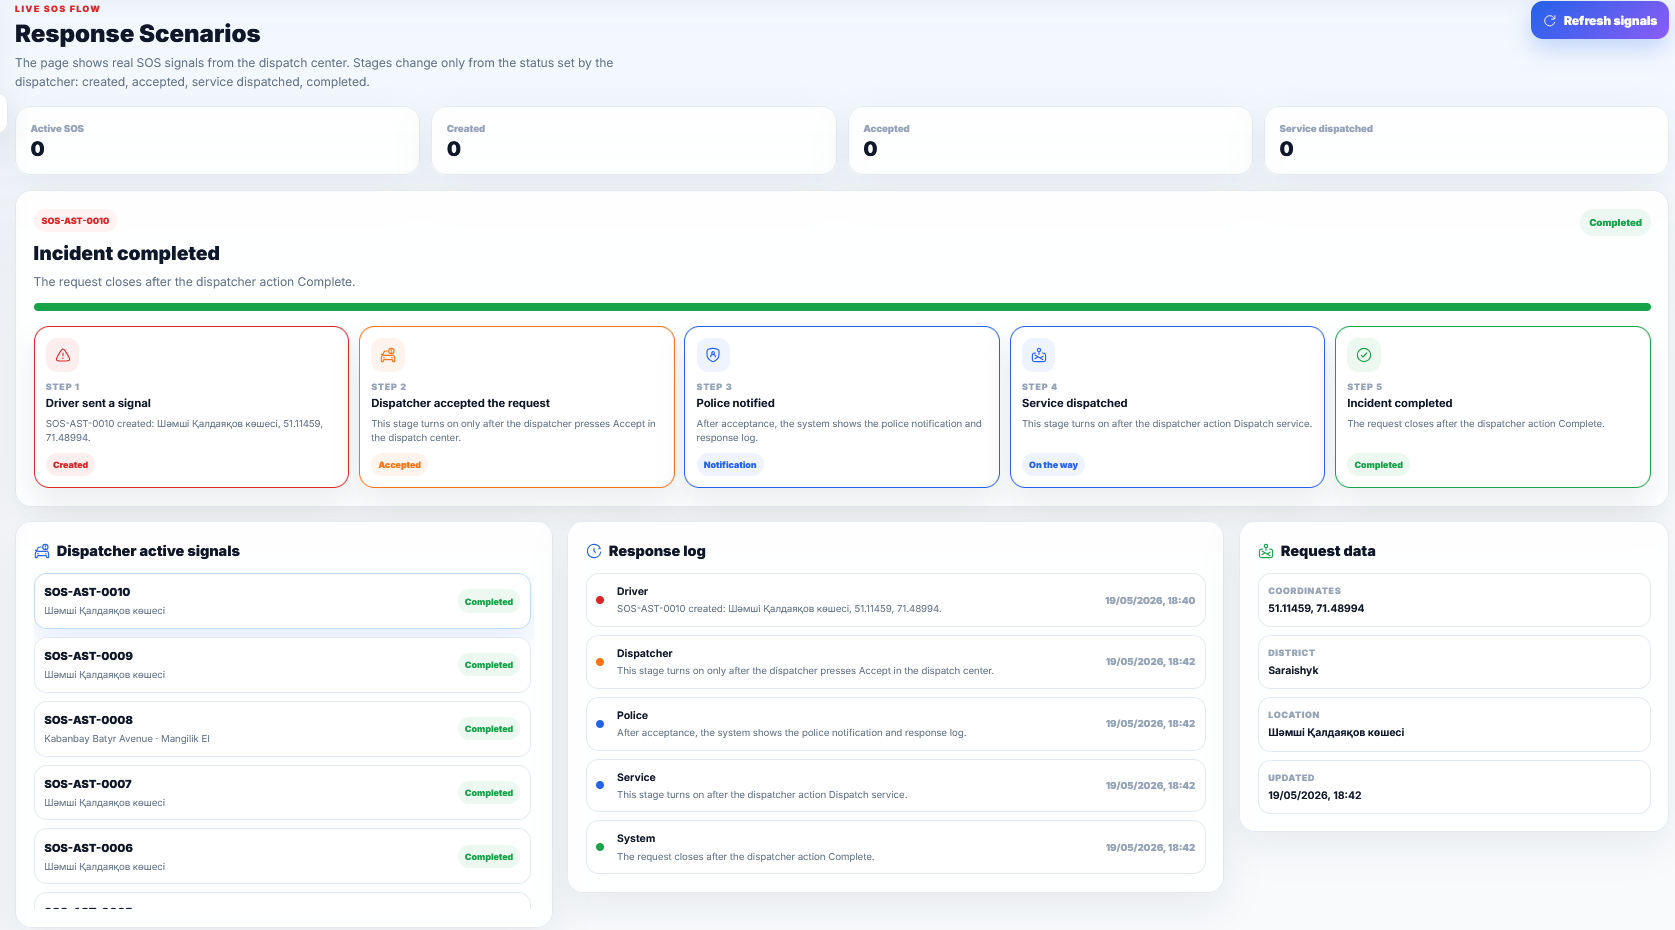
\includegraphics[width=\textwidth]{figures/response_scenarios_page.png}
\caption{Response scenarios}
\end{subfigure}
\caption{SOS operational workflow pages}
\label{fig:sos_operational_pages}
\end{figure}

These combined components show that AstanaSafe is more than a passive tool for viewing road accident statistics. With the SOS workflow, road safety data is connected with user roles, live incident status, geographic location and response logic. This expands AstanaSafe from a simple analytical interface into a prototype of a city decision support system for road safety.

\section{RoadVision AI Module}

RoadVision AI is deployed as an additional module of AstanaSafe. The main focus of the diploma project remains the web dashboard for accident statistics, congestion reports, dangerous zones and emergency response workflows. RoadVision extends the same platform from statistical visualization to video-based review of road incidents, but it is not treated as the central contribution of the project.

The module is implemented in the \texttt{RoadVision.jsx} page. When an accident video is uploaded, the interface allows the user to choose an analysis scenario, select or confirm the accident point on the map, and run video processing. The page contains a video preview, an event map, accident participants, a chronology block, risk indicators and a preliminary conclusion. This structure makes the module suitable for dispatcher-oriented review because the result is presented not as raw AI text, but as a structured incident card.

When the video is submitted for analysis, the frontend sends the uploaded file and related metadata to the backend through the RoadVision API. The request consists of the selected scenario, engine, location name, coordinates, interface language and the video file itself. The video is sent as multipart form data to the \texttt{/roadvision/analyze} endpoint. The backend also rejects videos larger than 250 MB in order to protect the server from processing overly large files during demonstration.

Several fallback layers are included in the backend processing logic. For each uploaded video, the system first checks whether a prepared analysis is already available. If such a result exists, it is returned immediately. If there is no prepared result, the system checks whether the selected engine allows external AI processing and then tries to analyze the video with Gemini Vision. If the external AI service is not available or does not respond in automatic mode, the backend returns a structured fallback analysis. This design keeps the module usable during demonstration even when external AI processing is unavailable.

The RoadVision result contains the selected location, video metadata, source of analysis, detected objects, confidence value, risk score and preliminary conclusion. The conclusion includes probable cause, estimated traffic impact and a participant with possible violation signs. The result also contains a timeline that describes the visible sequence of events by time. This output can be exported as a JSON report or prepared for dispatcher review together with forensic notes.

The implemented RoadVision interface is shown in Figure~\ref{fig:roadvision_pages}.

\begin{figure}[H]
\centering
\begin{subfigure}{0.49\textwidth}
\centering
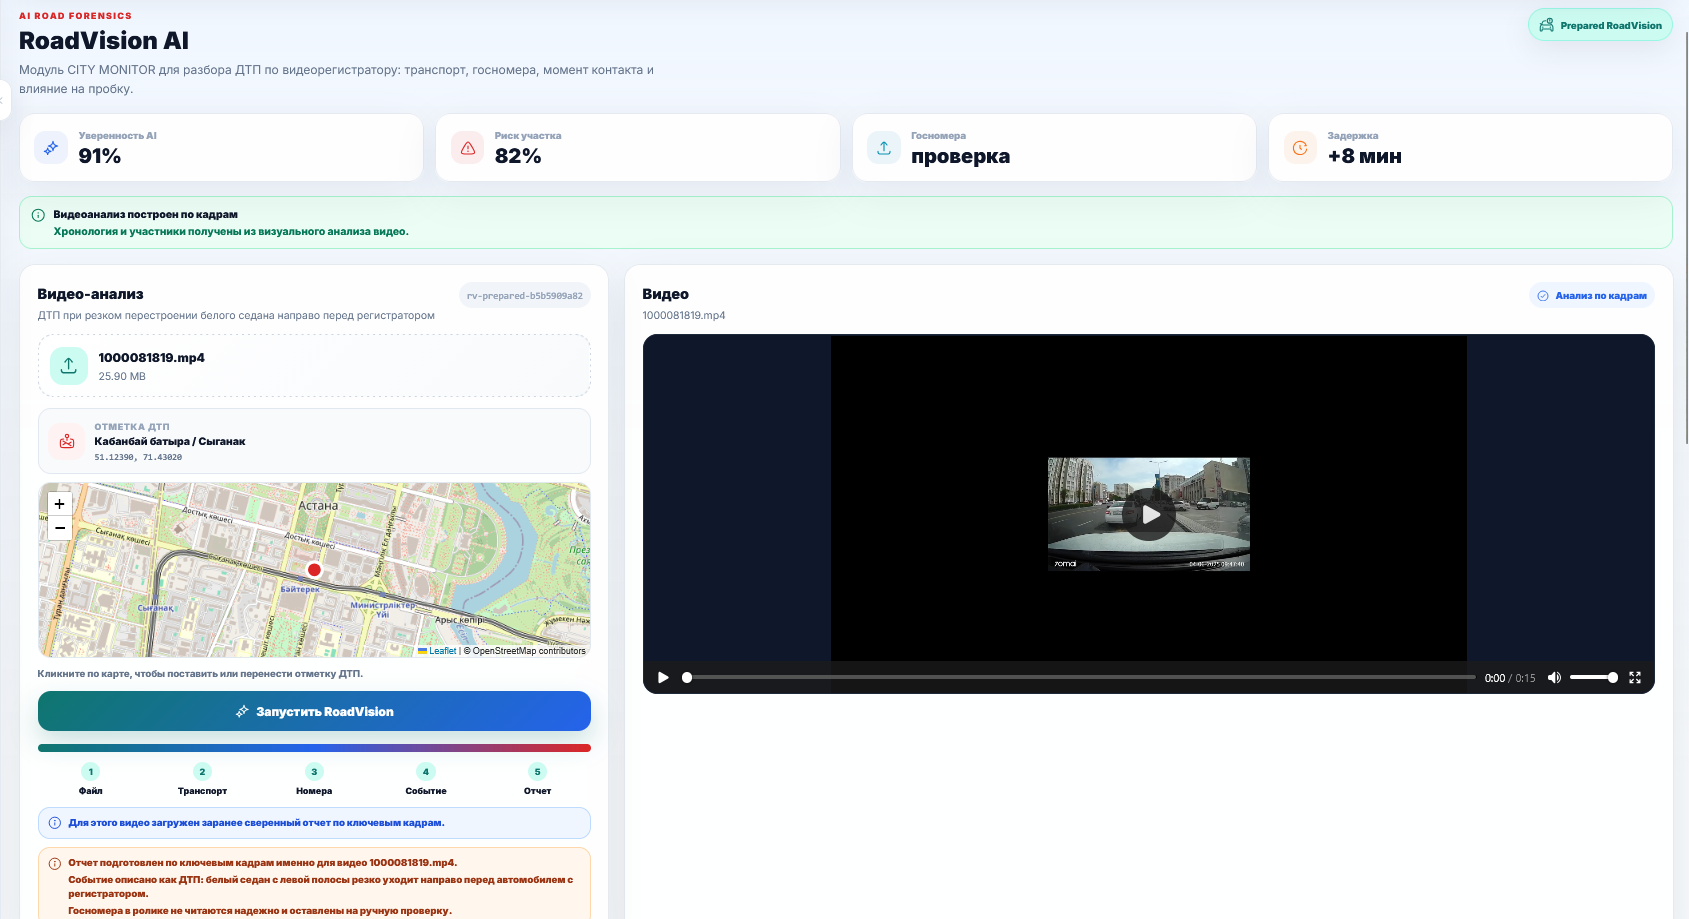
\includegraphics[width=\textwidth]{figures/roadvision_page.png}
\caption{Video upload and event map}
\end{subfigure}
\hfill
\begin{subfigure}{0.49\textwidth}
\centering
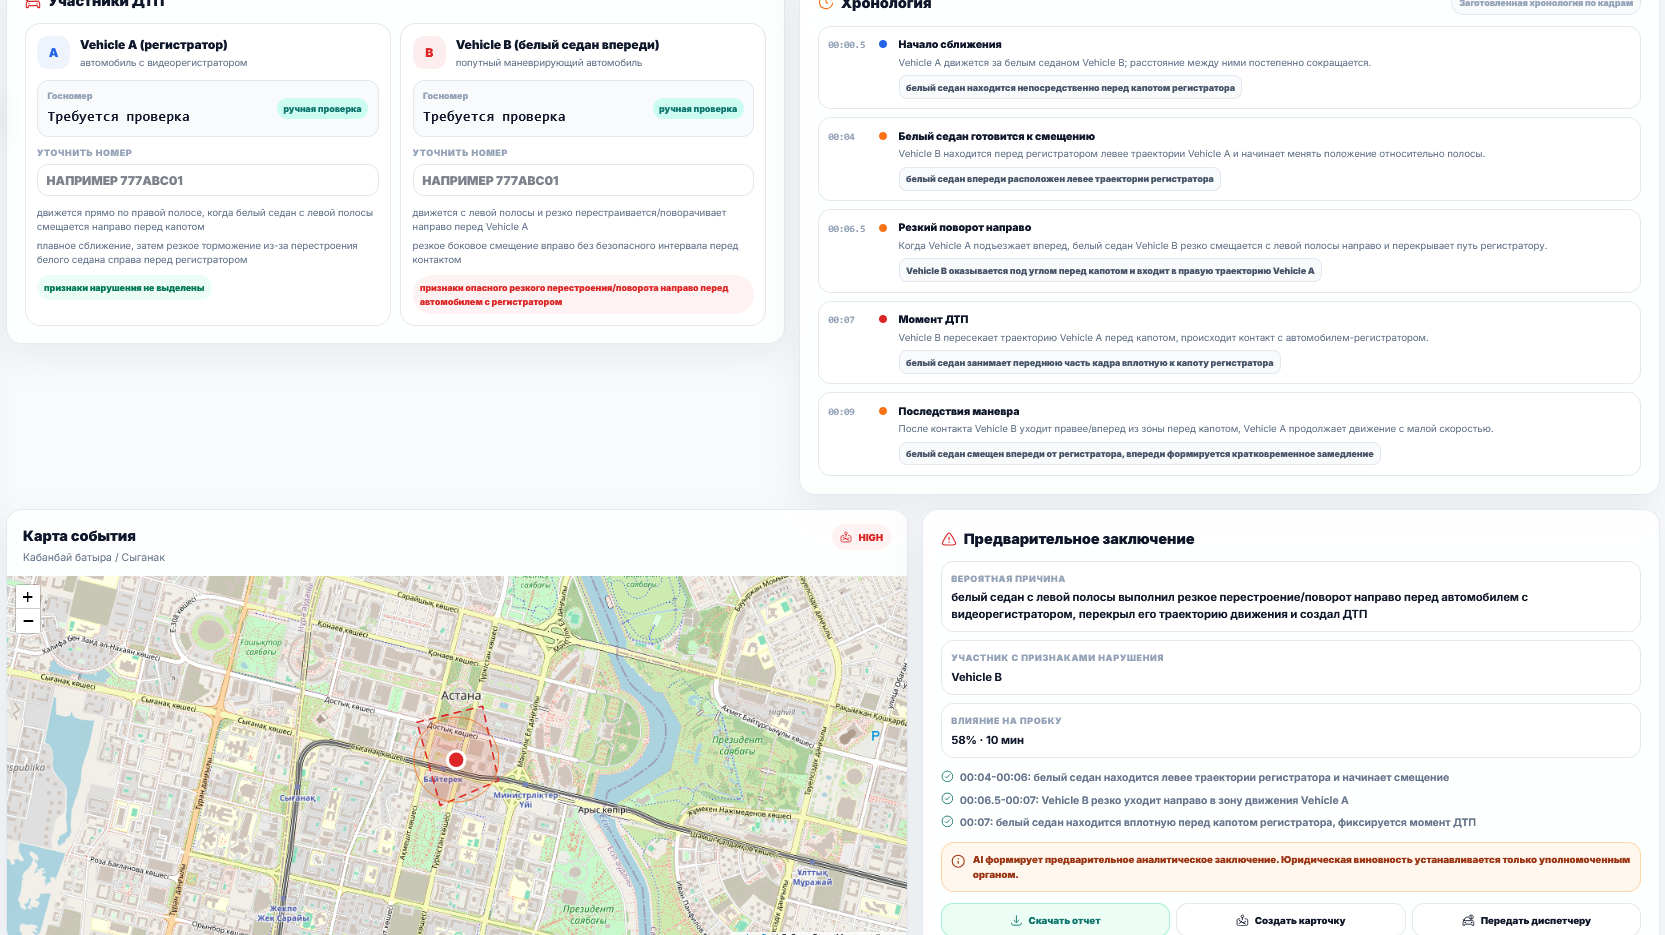
\includegraphics[width=\textwidth]{figures/roadvision_page_second.png}
\caption{RoadVision analysis result}
\end{subfigure}
\caption{RoadVision AI module interface}
\label{fig:roadvision_pages}
\end{figure}

The generated text is a draft technical review and should not be considered legal evidence. The quality of accident video analysis depends on video quality, visibility, camera angle and model availability. The value of RoadVision within the diploma project is that it demonstrates the extensibility of the AstanaSafe platform. The same system can combine historical accident data, user-generated traffic reports, SOS workflows and video-assisted incident review \cite{kitchin2014}. This type of extension is consistent with broader smart city systems where data sources and operational services are combined within one urban platform \cite{batty2012}.

The implementation of RoadVision supports the practical contribution of the project by showing that AstanaSafe can be developed as a larger road safety decision support system. The module connects a video file with a map point, structured incident description, risk score and dispatcher-oriented output. This expands the application beyond maps and tables while keeping RoadVision as an additional module rather than the main focus of the system.

\clearpage
\chapter*{Conclusion}
\addcontentsline{toc}{chapter}{Conclusion}

The diploma project deals with the problem of fragmented information on road safety in Astana. There are various data sources that contain historical information on accidents, user-submitted congestion reports, district information and ongoing operational incidents. These pieces of information are usually stored or viewed separately from each other. It is therefore difficult to gain insight into where accidents are repeated, where problems need to be addressed and how analysis can support concrete workflows for handling incidents.

The result of the diploma work is the implementation of the AstanaSafe web application, which is a city decision support system for road safety. An interactive map, accident statistics, traffic reports, charts and tables, dangerous area ranking, district passports, SOS workflow, dispatcher panel, emergency response scenarios and the additional RoadVision AI module were implemented on the basis of practical tasks. The system is a client-server application, implemented using React and Vite on the client side, FastAPI on the server side and PostgreSQL as the main database.

The project is based on historical road accident data from the public KPSSU/DTP ArcGIS REST layer. These records were filtered for Astana, transformed into a local GeoJSON dataset and loaded into the \texttt{real\_accidents} table \cite{kpssuDtp}. The project also uses road and district context data preprocessed from OpenStreetMap data provided by Geofabrik. User-submitted congestion and incident reports are stored separately in the \texttt{traffic\_reports} table. This separation makes it possible to compare long-term accident history with current reports from users without mixing their origin.

The main achievement of this diploma project is the integration of several road safety functions into one web platform. The system does not simply display points on a map. It links accident history with user reports, districts, roads, filters, charts and risk indicators. The District Passport and Danger Zones pages enable a shift from isolated incidents to area-based interpretation. Dispatcher and SOS workflows demonstrate how the system can support incident coordination. RoadVision AI demonstrates how the platform can be extended with video-assisted review, while remaining an additional module rather than the central part of the diploma project.

The completed system meets the main goal of the diploma project, which is to design a web dashboard for road accident statistics and congestion in Astana. The data can be filtered by district, date, accident type, user report, weather condition and severity. The project shows that open and prepared geospatial data can be transformed into a useful interface rather than remaining as separate tables or raw GIS files \cite{goodchild2007}.

The project has several limitations. User-submitted congestion data depends on how many reports are submitted and how accurately they describe the road situation. The system does not use an official real-time traffic data provider and is not intended as a replacement for professional emergency services or transport planning tools. The output from RoadVision AI represents a draft technical result that requires human validation. These limitations do not take away from the value of the project, because the aim was to develop a working city-specific dashboard prototype rather than a fully operational commercial navigation system or emergency platform.

Potential future work may include integration with traffic sensors, more precise accident type grading, more advanced spatial clustering algorithms, mobile support, refined user report verification and deeper integration with city services. The existing project is an initial implementation for these possible improvements, with the system already separated into frontend, backend, database, analytical services and operational modules.

\clearpage
\addcontentsline{toc}{chapter}{Bibliography}
\begin{thebibliography}{99}

\bibitem{who2023}
World Health Organization. \emph{Global Status Report on Road Safety 2023}.
\url{https://www.who.int/publications/i/item/9789240086517}, 2023.

\bibitem{fhwa2015}
Federal Highway Administration. \emph{Incorporating Travel-Time Reliability into the Congestion Management Process (CMP): A Primer}.
\url{https://ops.fhwa.dot.gov/publications/fhwahop14034/index.htm}, 2015.

\bibitem{anderson2009}
Anderson, T. K. Kernel density estimation and K-means clustering to profile road accident hotspots. \emph{Accident Analysis and Prevention}, 41(3), 359--364, 2009.

\bibitem{xie2013}
Xie, Z., and Yan, J. Detecting traffic accident clusters with network kernel density estimation and local spatial statistics: an integrated approach. \emph{Journal of Transport Geography}, 31, 64--71, 2013.

\bibitem{elvik2008}
Elvik, R. A survey of operational definitions of hazardous road locations in some European countries. \emph{Accident Analysis and Prevention}, 40(6), 1830--1835, 2008.

\bibitem{erdogan2008}
Erdogan, S., Yilmaz, I., Baybura, T., and Gullu, M. Geographical information systems aided traffic accident analysis system: case study of Afyonkarahisar. \emph{Accident Analysis and Prevention}, 40(1), 174--181, 2008.

\bibitem{lord2010}
Lord, D., and Mannering, F. The statistical analysis of crash-frequency data: a review and assessment of methodological alternatives. \emph{Transportation Research Part A: Policy and Practice}, 44(5), 291--305, 2010.

\bibitem{flahaut2003}
Flahaut, B., Mouchart, M., San Martin, E., and Thomas, I. The local spatial autocorrelation and the kernel method for identifying black zones: a comparative approach. \emph{Accident Analysis and Prevention}, 35(6), 991--1004, 2003.

\bibitem{anselin1995}
Anselin, L. Local indicators of spatial association: LISA. \emph{Geographical Analysis}, 27(2), 93--115, 1995.

\bibitem{goodchild2007}
Goodchild, M. F. Citizens as sensors: the world of volunteered geography. \emph{GeoJournal}, 69(4), 211--221, 2007.

\bibitem{kitchin2014}
Kitchin, R. The real-time city? Big data and smart urbanism. \emph{GeoJournal}, 79(1), 1--14, 2014.

\bibitem{batty2012}
Batty, M., Axhausen, K. W., Giannotti, F., Pozdnoukhov, A., Bazzani, A., Wachowicz, M., Ouzounis, G., and Portugali, Y. Smart cities of the future. \emph{The European Physical Journal Special Topics}, 214, 481--518, 2012.

\bibitem{chourabi2012}
Chourabi, H., Nam, T., Walker, S., Gil-Garcia, J. R., Mellouli, S., Nahon, K., Pardo, T. A., and Scholl, H. J. Understanding smart cities: an integrative framework. \emph{Proceedings of the 45th Hawaii International Conference on System Sciences}, 2289--2297, 2012.

\bibitem{few2006}
Few, S. \emph{Information Dashboard Design: The Effective Visual Communication of Data}. Sebastopol: O'Reilly Media, 2006.

\bibitem{shneiderman1996}
Shneiderman, B. The eyes have it: a task by data type taxonomy for information visualizations. \emph{Proceedings of the IEEE Symposium on Visual Languages}, 336--343, 1996.

\bibitem{chen2012}
Chen, H., Chiang, R. H. L., and Storey, V. C. Business intelligence and analytics: from big data to big impact. \emph{MIS Quarterly}, 36(4), 1165--1188, 2012.

\bibitem{ewing2009}
Ewing, R., and Dumbaugh, E. The built environment and traffic safety: a review of empirical evidence. \emph{Journal of Planning Literature}, 23(4), 347--367, 2009.

\bibitem{tempelmeier2020}
Tempelmeier, N., Sander, A., Feuerhake, U., Lohdefink, M., and Demidova, E. TA-Dash: an interactive dashboard for spatial-temporal traffic analytics. \emph{Proceedings of the 28th ACM SIGSPATIAL International Conference on Advances in Geographic Information Systems}, 2020.

\bibitem{tufte2001}
Tufte, E. R. \emph{The Visual Display of Quantitative Information}. 2nd ed. Cheshire: Graphics Press, 2001.

\bibitem{ware2012}
Ware, C. \emph{Information Visualization: Perception for Design}. 3rd ed. Waltham: Morgan Kaufmann, 2012.

\bibitem{wilkinson2005}
Wilkinson, L. \emph{The Grammar of Graphics}. 2nd ed. New York: Springer, 2005.

\bibitem{andrienko2013}
Andrienko, N., and Andrienko, G. Visual analytics of movement: an overview of methods, tools and procedures. \emph{Information Visualization}, 12(1), 3--24, 2013.

\bibitem{atluri2018}
Atluri, G., Karpatne, A., and Kumar, V. Spatio-temporal data mining: a survey of problems and methods. \emph{ACM Computing Surveys}, 51(4), Article 83, 2018.

\bibitem{vlahogianni2014}
Vlahogianni, E. I., Karlaftis, M. G., and Golias, J. C. Short-term traffic forecasting: where we are and where we are going. \emph{Transportation Research Part C: Emerging Technologies}, 43, 3--19, 2014.

\bibitem{kpssuDtp}
KPSSU. Public ArcGIS REST layer KPSSU/DTP, layer ``DTP''.
\url{https://gis.kgp.kz/arcgis/rest/services/KPSSU/DTP/FeatureServer/layers}, 2026.

\bibitem{geofabrikKazakhstan}
Geofabrik. \emph{Kazakhstan OpenStreetMap Data Extracts}.
\url{https://download.geofabrik.de/asia/kazakhstan.html}, 2026.

\bibitem{osmCopyright}
OpenStreetMap contributors. \emph{OpenStreetMap Copyright and License}.
\url{https://www.openstreetmap.org/copyright}, 2026.

\bibitem{leafletDocs}
Leaflet. \emph{Leaflet Documentation}.
\url{https://leafletjs.com/reference.html}, 2026.

\bibitem{twogisHelp}
2GIS. \emph{Traffic alerts and road events in 2GIS}.
\url{https://help.2gis.com/question/how-to-see-traffic-alerts-in-2gis}, 2026.

\bibitem{yandexMapsHelp}
Yandex. \emph{Traffic and road events in Yandex Maps}.
\url{https://yandex.com/support/m-maps/en/jams}, 2026.

\bibitem{googleMapsNavigation}
Google. \emph{Use navigation in Google Maps}.
\url{https://support.google.com/maps/answer/3273406}, 2026.

\end{thebibliography}

\clearpage
\appendix
\titleformat{\chapter}[block]
  {\normalfont\fontsize{14}{16.8}\bfseries}
  {Appendix~\thechapter.~}{0em}{}

\chapter*{Appendix A}
\addcontentsline{toc}{chapter}{Appendix A. Interview Evidence: Segment A and Segment B}
\refstepcounter{chapter}
\setcounter{figure}{0}

\section*{Interview Evidence: Segment A and Segment B}

This appendix presents screenshots of the semi-structured interviews conducted in January 2026 with stakeholders from Segments A and B. The screenshots for each participant are displayed in consecutive order, capturing the interview process as it unfolded. Segments C, urban planners and researchers, and D, drivers and commuters, were recorded in audio format only; therefore, no screenshots are presented for these stakeholder groups.

\section*{Segment A - City Transport and Road Infrastructure Specialists}

The feedback from Segment A was mainly provided by students and professionals who work in the field of urban mobility, transport engineering and road safety policy. During the interviews, they were asked about their current data sources, the most relevant attributes, and the analytical functionality they would prioritise in a dedicated traffic dashboard.

\subsection*{Respondent A1 - Transport Engineering Student}

\begin{figure}[H]
\centering

\includegraphics[width=0.24\textwidth]{figures/1.1.png}
\hspace{0.16\textwidth}

\includegraphics[width=0.24\textwidth]{figures/1.2.png}

\vspace{0.35cm}

\includegraphics[width=0.24\textwidth]{figures/1.3.png}
\hspace{0.16\textwidth}

\includegraphics[width=0.24\textwidth]{figures/1.4.png}
\caption{Interview with Respondent A1}
\label{fig:appendix_interview_a1}
\end{figure}

\subsection*{Respondent A2 - Urban Planning Student}

\begin{figure}[H]
\centering

\includegraphics[width=0.24\textwidth]{figures/2.1.png}
\hspace{0.16\textwidth}

\includegraphics[width=0.24\textwidth]{figures/2.2.png}

\vspace{0.35cm}

\includegraphics[width=0.24\textwidth]{figures/2.3.png}
\hspace{0.16\textwidth}

\includegraphics[width=0.24\textwidth]{figures/2.4.png}
\caption{Interview with Respondent A2}
\label{fig:appendix_interview_a2}
\end{figure}

\subsection*{Respondent A3 - Road Infrastructure Intern}

\begin{figure}[H]
\centering

\includegraphics[width=0.21\textwidth]{figures/3.1.png}
\hspace{0.08\textwidth}

\includegraphics[width=0.21\textwidth]{figures/3.2.png}
\hspace{0.08\textwidth}

\includegraphics[width=0.21\textwidth]{figures/3.3.png}

\vspace{0.35cm}

\includegraphics[width=0.21\textwidth]{figures/3.4.png}
\hspace{0.18\textwidth}

\includegraphics[width=0.21\textwidth]{figures/3.5.png}
\caption{Interview with Respondent A3}
\label{fig:appendix_interview_a3}
\end{figure}

\section*{Segment B - Monitoring and Dispatch Users}

Segment B consisted of participants with experience in call-centres, dispatch environments and monitoring workflows. Some participants also had experience with active operations. For this segment, information channels, operational data attributes and important features of a centralised incident dashboard were identified.

\subsection*{Respondent B1 - Call Centre / Monitoring Student}

\begin{figure}[H]
\centering

\includegraphics[width=0.24\textwidth]{figures/4.1.png}
\hspace{0.16\textwidth}

\includegraphics[width=0.24\textwidth]{figures/4.2.png}

\vspace{0.35cm}

\includegraphics[width=0.24\textwidth]{figures/4.3.png}
\hspace{0.16\textwidth}

\includegraphics[width=0.24\textwidth]{figures/4.4.png}
\caption{Interview with Respondent B1}
\label{fig:appendix_interview_b1}
\end{figure}

\subsection*{Respondent B2 - Public Service Dispatch Intern}

\begin{figure}[H]
\centering

\includegraphics[width=0.21\textwidth]{figures/5.1.png}
\hspace{0.08\textwidth}

\includegraphics[width=0.21\textwidth]{figures/5.2.png}
\hspace{0.08\textwidth}

\includegraphics[width=0.21\textwidth]{figures/5.3.png}

\vspace{0.35cm}

\includegraphics[width=0.21\textwidth]{figures/5.4.png}
\hspace{0.18\textwidth}

\includegraphics[width=0.21\textwidth]{figures/5.5.png}
\caption{Interview with Respondent B2}
\label{fig:appendix_interview_b2}
\end{figure}

\section*{Note on Segments C and D}

Interviews with participants in Segment C, urban planners and researchers, and Segment D, drivers and commuters, were conducted in audio format only. Permission or technical access for screen-recorded interviews was not available for these segments. Their data is analyzed in the narrative and quantitative analysis in Sections 1.4.3 and 1.4.4 of the thesis.

\clearpage
\chapter{AstanaSafe Interface Snapshots}

Appendix B contains screenshots of the AstanaSafe web application developed as part of the diploma project. The screenshots confirm that the project was not limited to theoretical system design, but also included the implemented interface of the main functional modules.

The Dashboard screenshot shows the main page of the web application with an interactive map, filters, road safety indicators and accident markers. The Analytics and Reports screenshots show how accident and traffic statistics are transformed into charts, indicators and tables sorted by selected criteria. The traffic report modal shows the form used for submitting road congestion or accident reports.

Appendix B contains several screenshots of the AstanaSafe web application. The screenshots of Danger Zones and District Passport modules illustrate a system for accumulation and organization of accidents and reports by risk-prone areas and districts. Dispatcher and Response Scenarios illustrate the system’s operational part where SOS incidents are monitored and processed. Additional screenshots of RoadVision application demonstrate an AI based system for reviewing accident video. A user of such a system can get a structured report of the accident with a link to a corresponding map point.

All functions of AstanaSafe web application that described in Chapter 3 of Practical Part were successfully implemented on its interface in order to be presented on defense of the diploma work.

\begin{figure}[H]
\centering
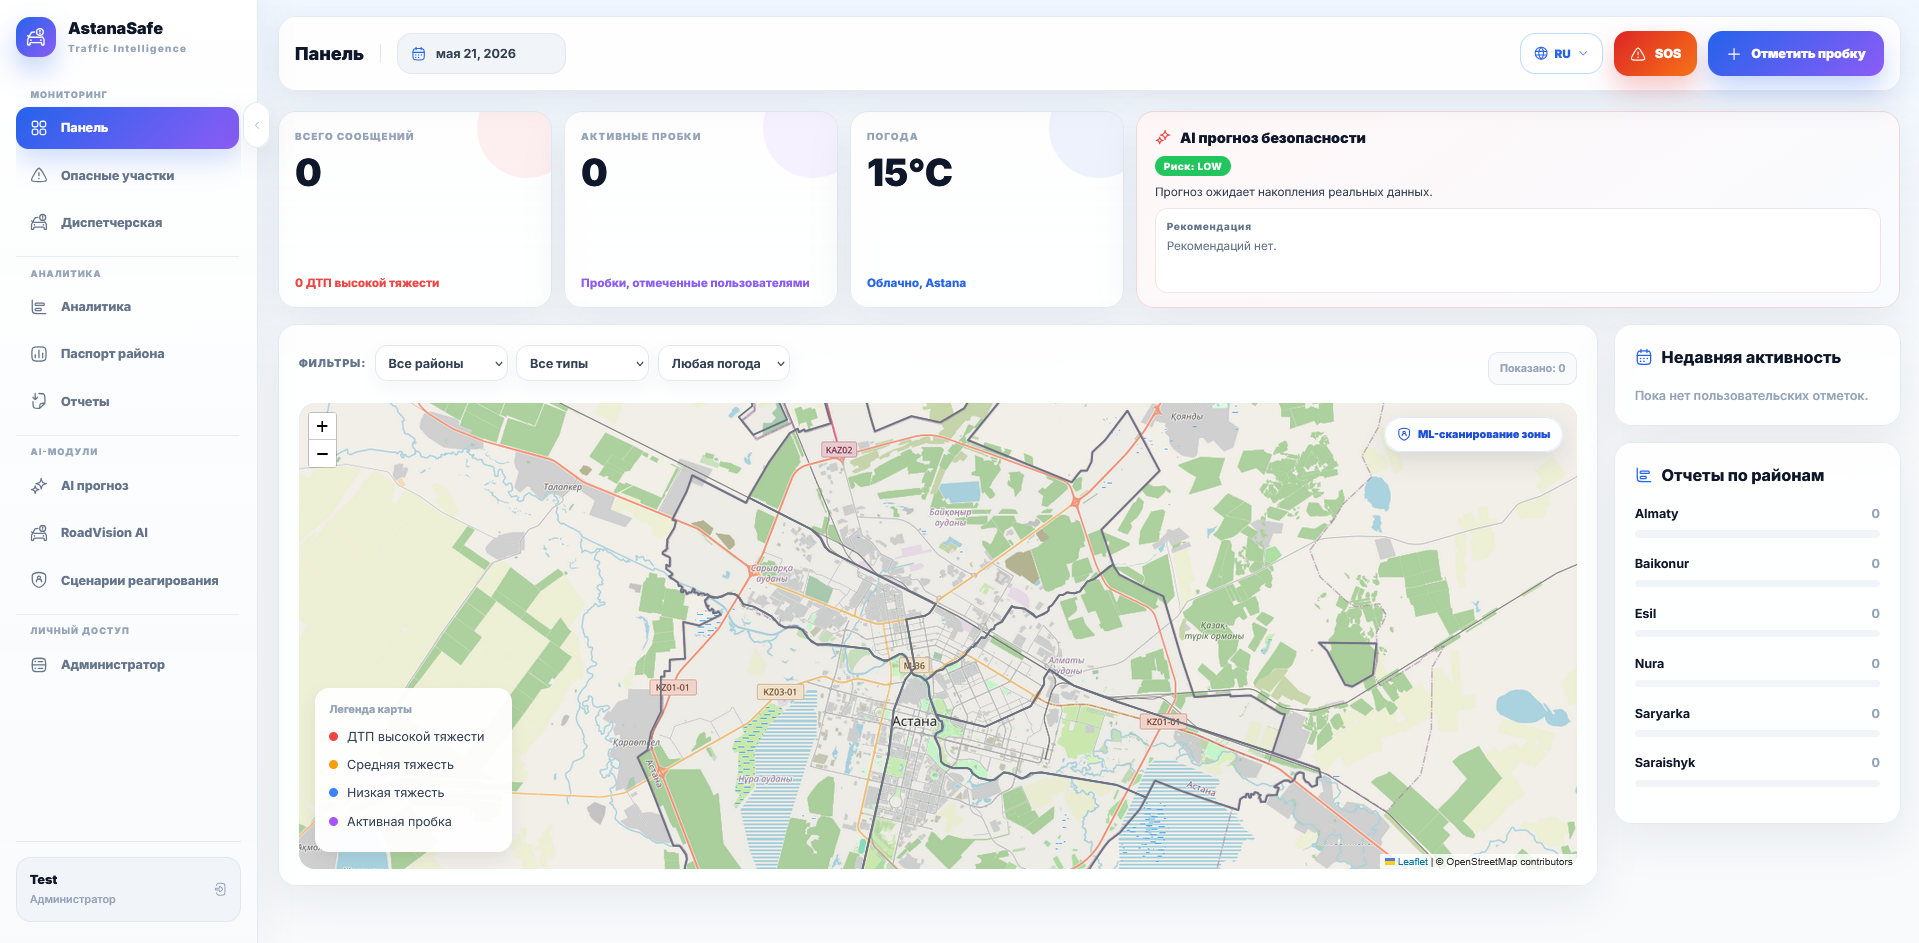
\includegraphics[width=\textwidth]{figures/dashboard_main_page.png}
\caption{Dashboard page of AstanaSafe}
\label{fig:appendix_dashboard}
\end{figure}

\begin{figure}[H]
\centering
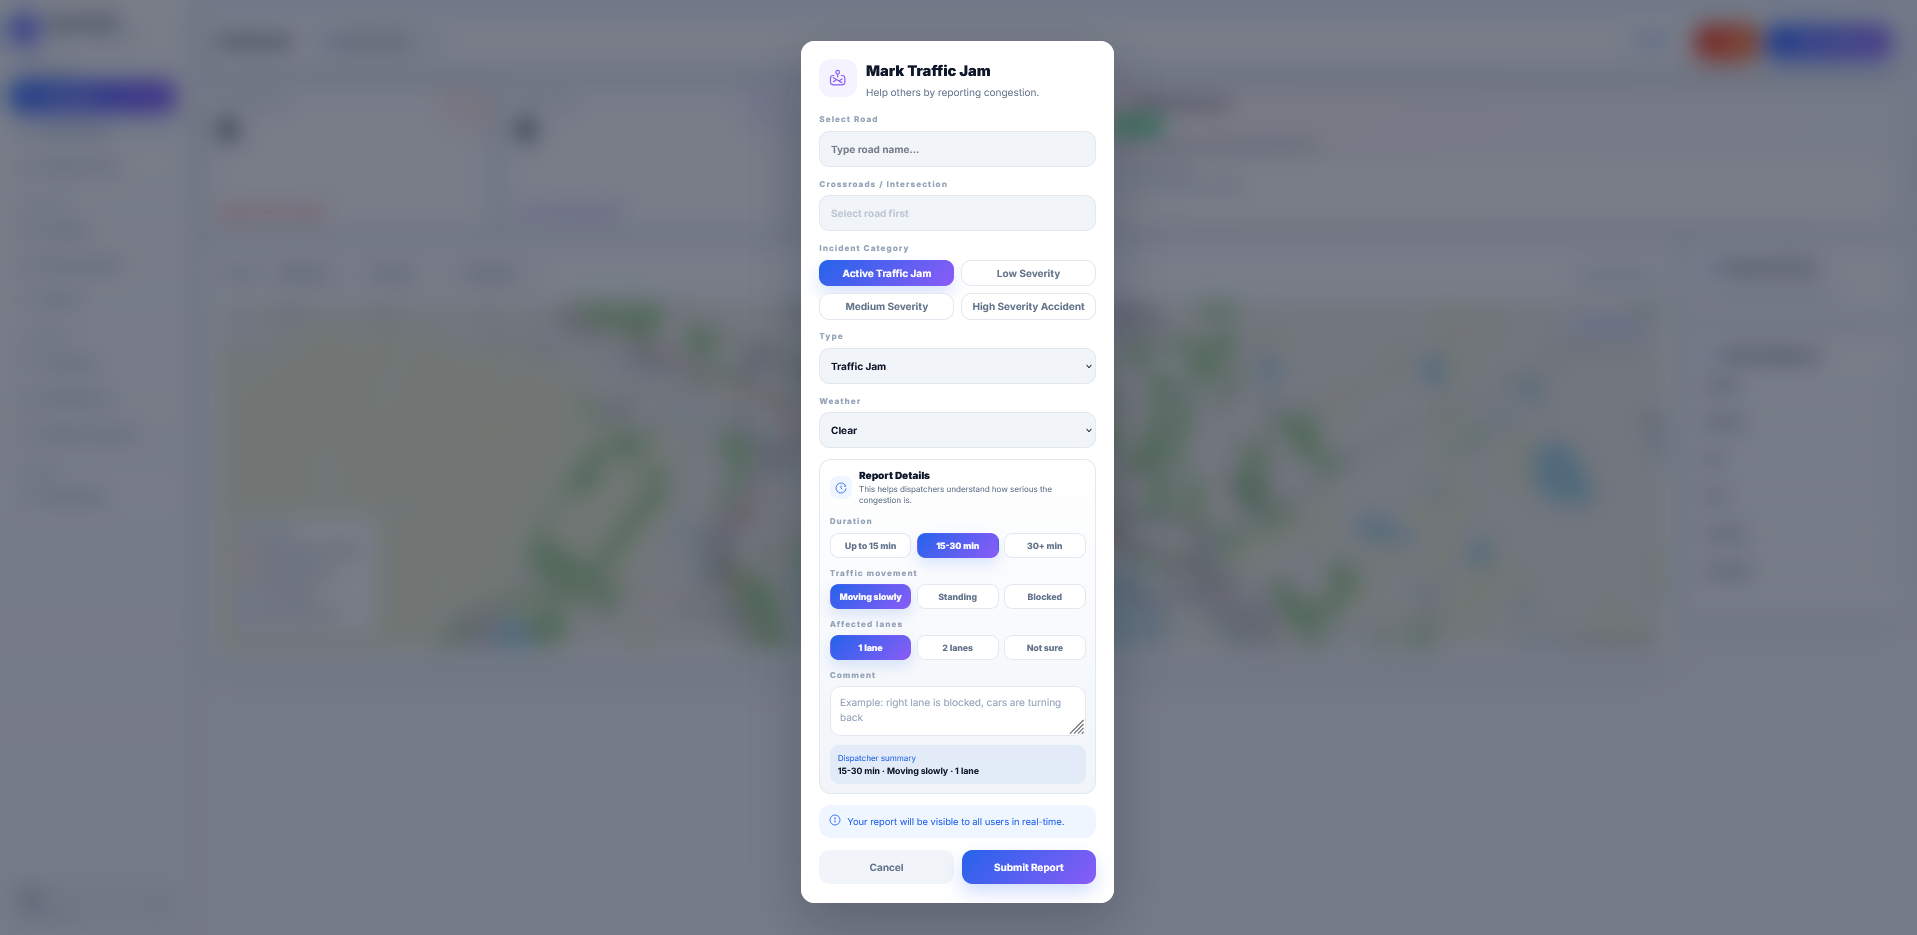
\includegraphics[width=\textwidth]{figures/traffic_report_modal.png}
\caption{Traffic report modal}
\label{fig:appendix_traffic_report_modal}
\end{figure}

\begin{figure}[H]
\centering
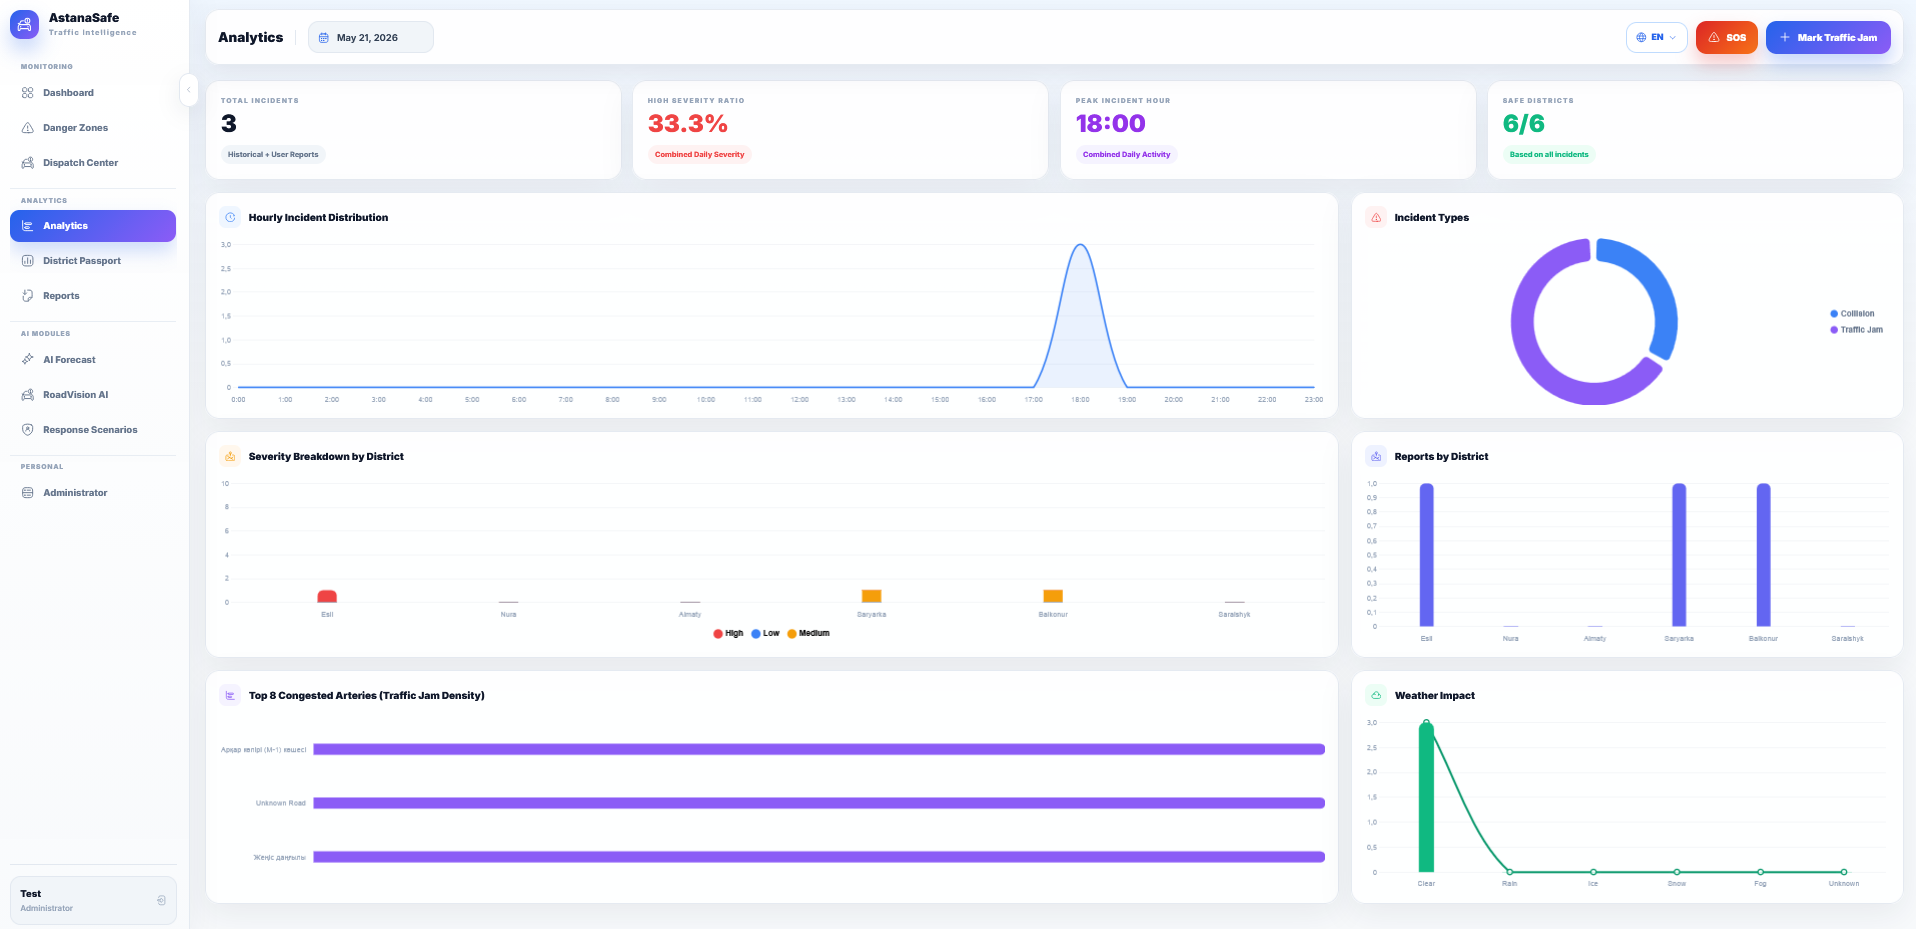
\includegraphics[width=\textwidth]{figures/analytics_page.png}
\caption{Analytics page}
\label{fig:appendix_analytics}
\end{figure}

\begin{figure}[H]
\centering
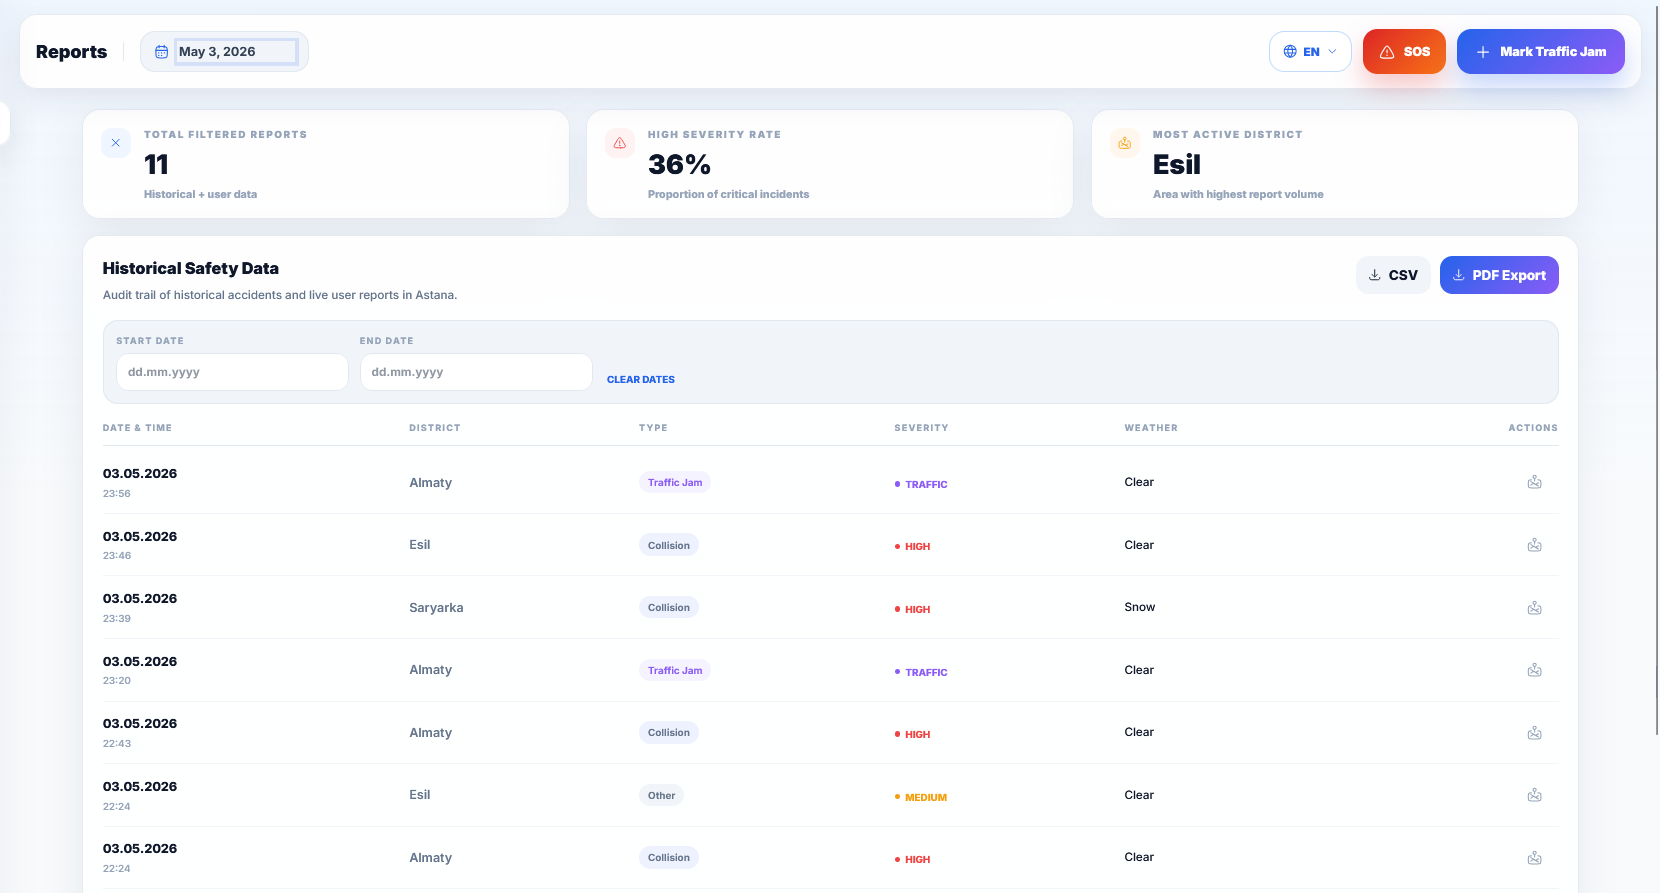
\includegraphics[width=\textwidth]{figures/reports_page.png}
\caption{Reports page}
\label{fig:appendix_reports}
\end{figure}

\begin{figure}[H]
\centering
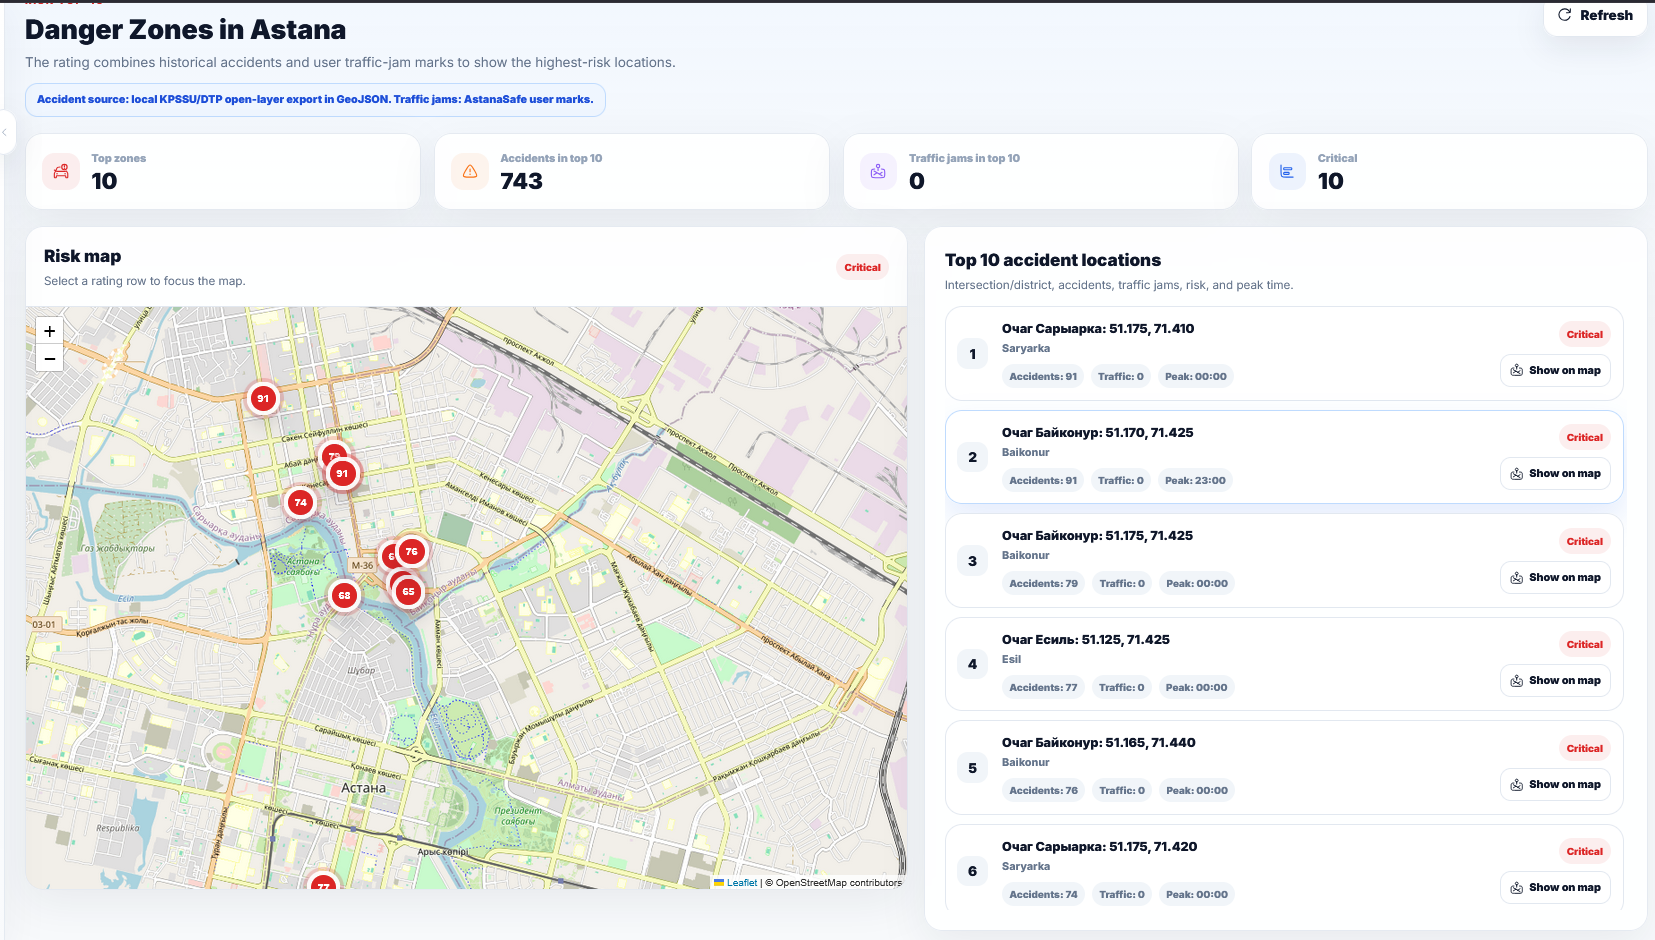
\includegraphics[width=\textwidth]{figures/danger_zones_page.png}
\caption{Danger Zones page}
\label{fig:appendix_danger_zones}
\end{figure}

\begin{figure}[H]
\centering
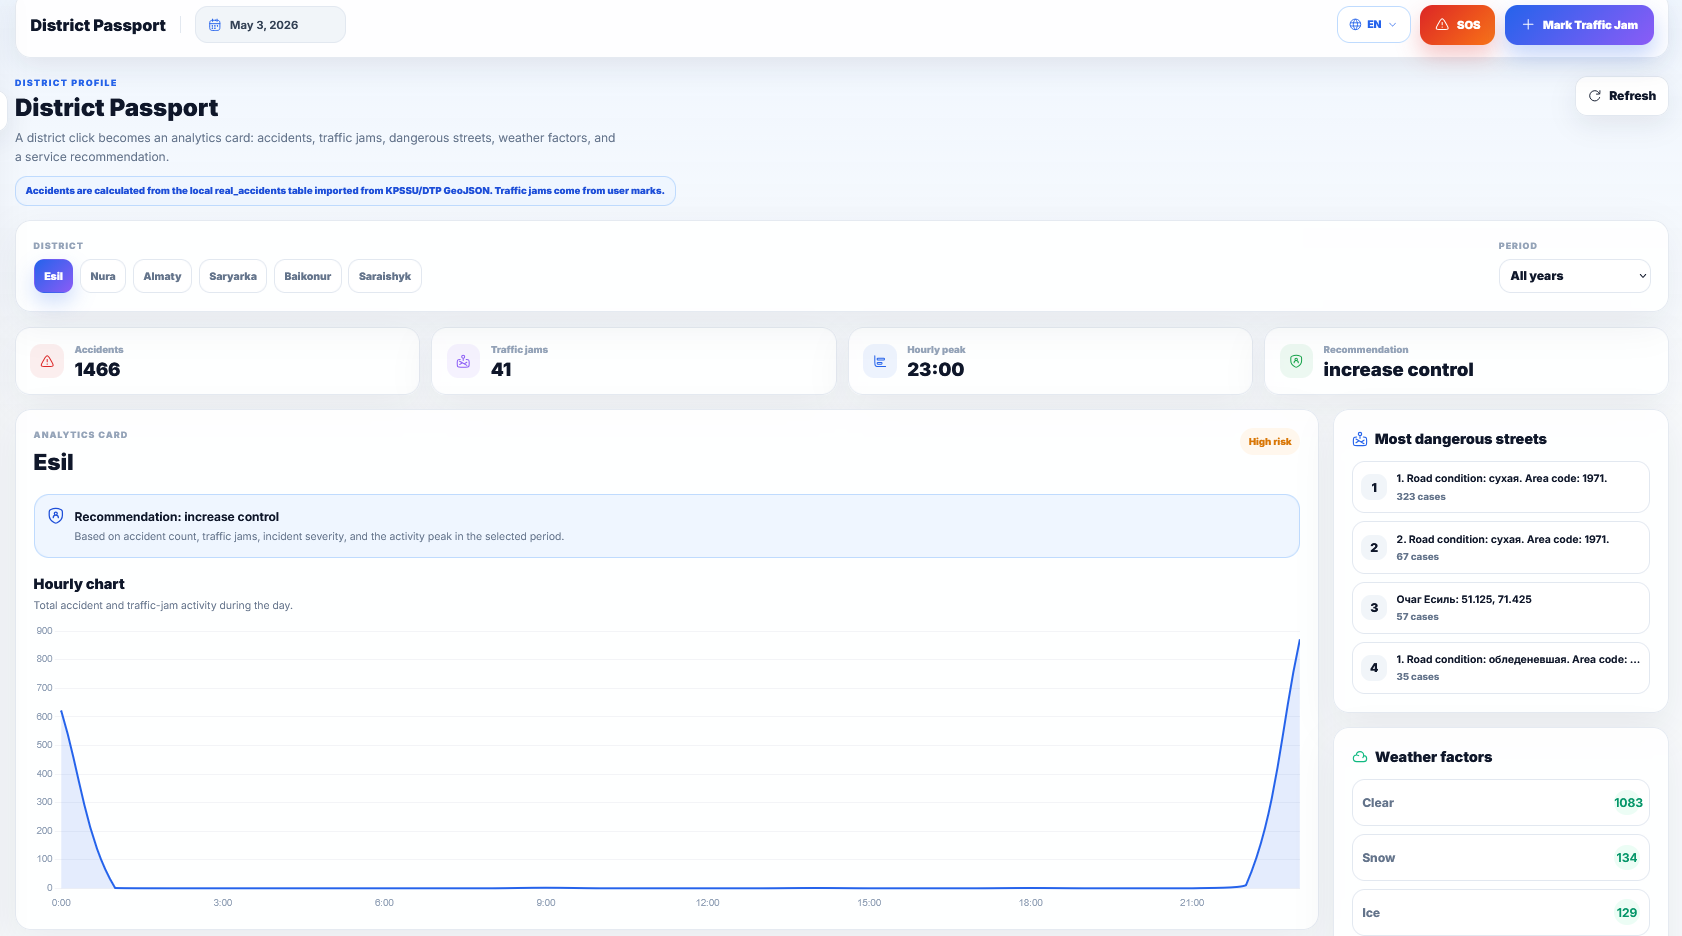
\includegraphics[width=\textwidth]{figures/district_passport_page.png}
\caption{District Passport page}
\label{fig:appendix_district_passport}
\end{figure}

\begin{figure}[H]
\centering
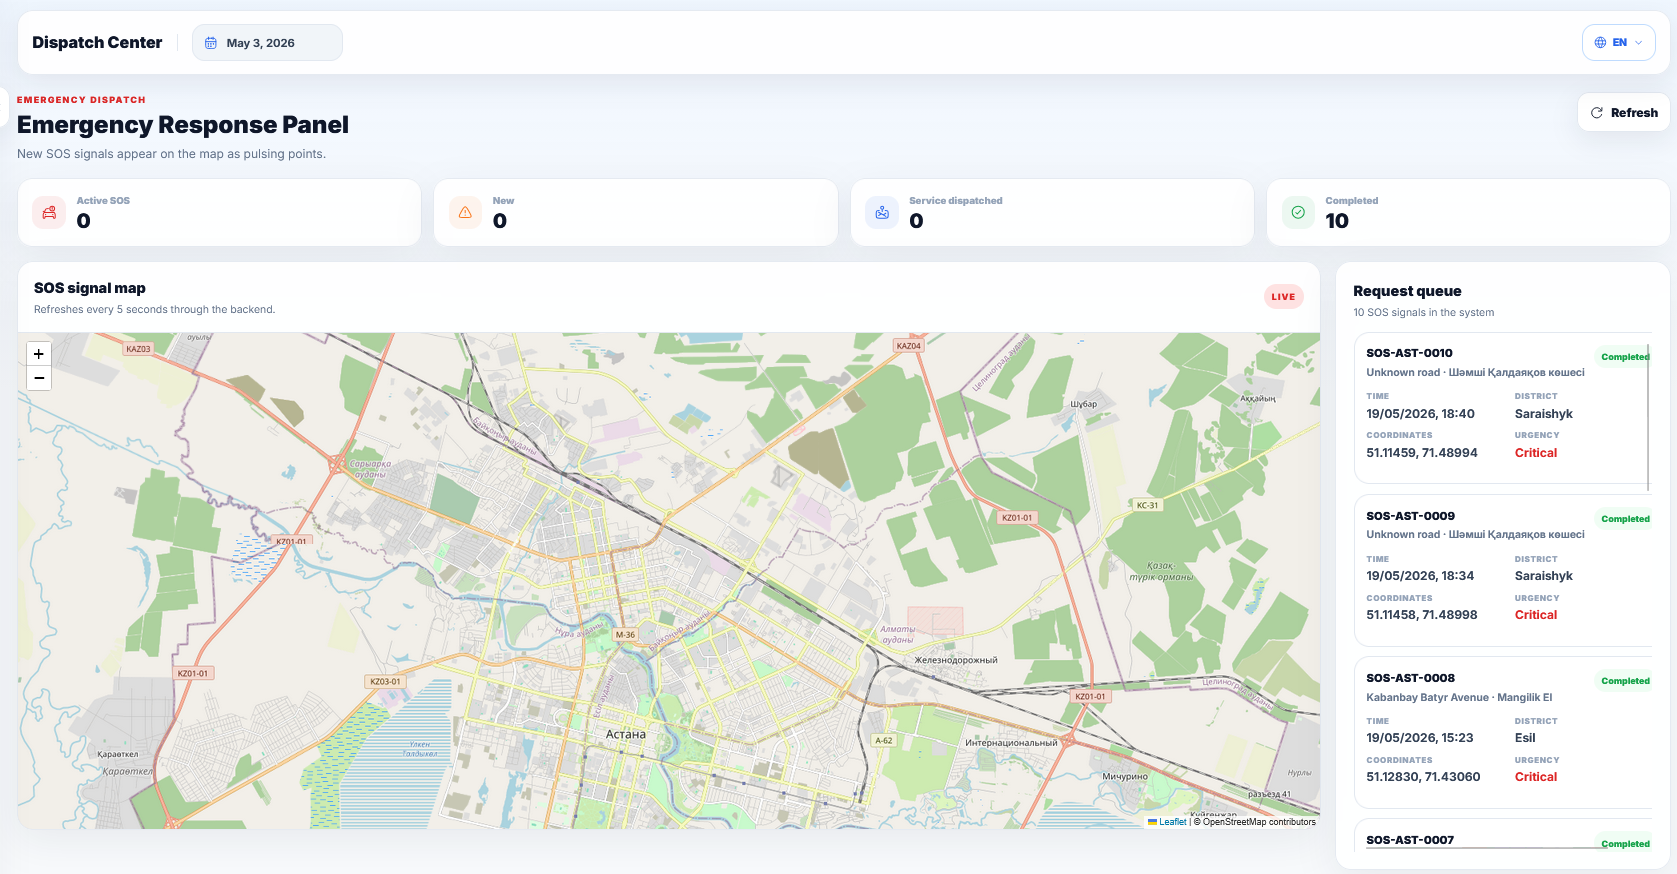
\includegraphics[width=\textwidth]{figures/dispatcher_page.png}
\caption{Dispatcher panel}
\label{fig:appendix_dispatcher}
\end{figure}

\begin{figure}[H]
\centering
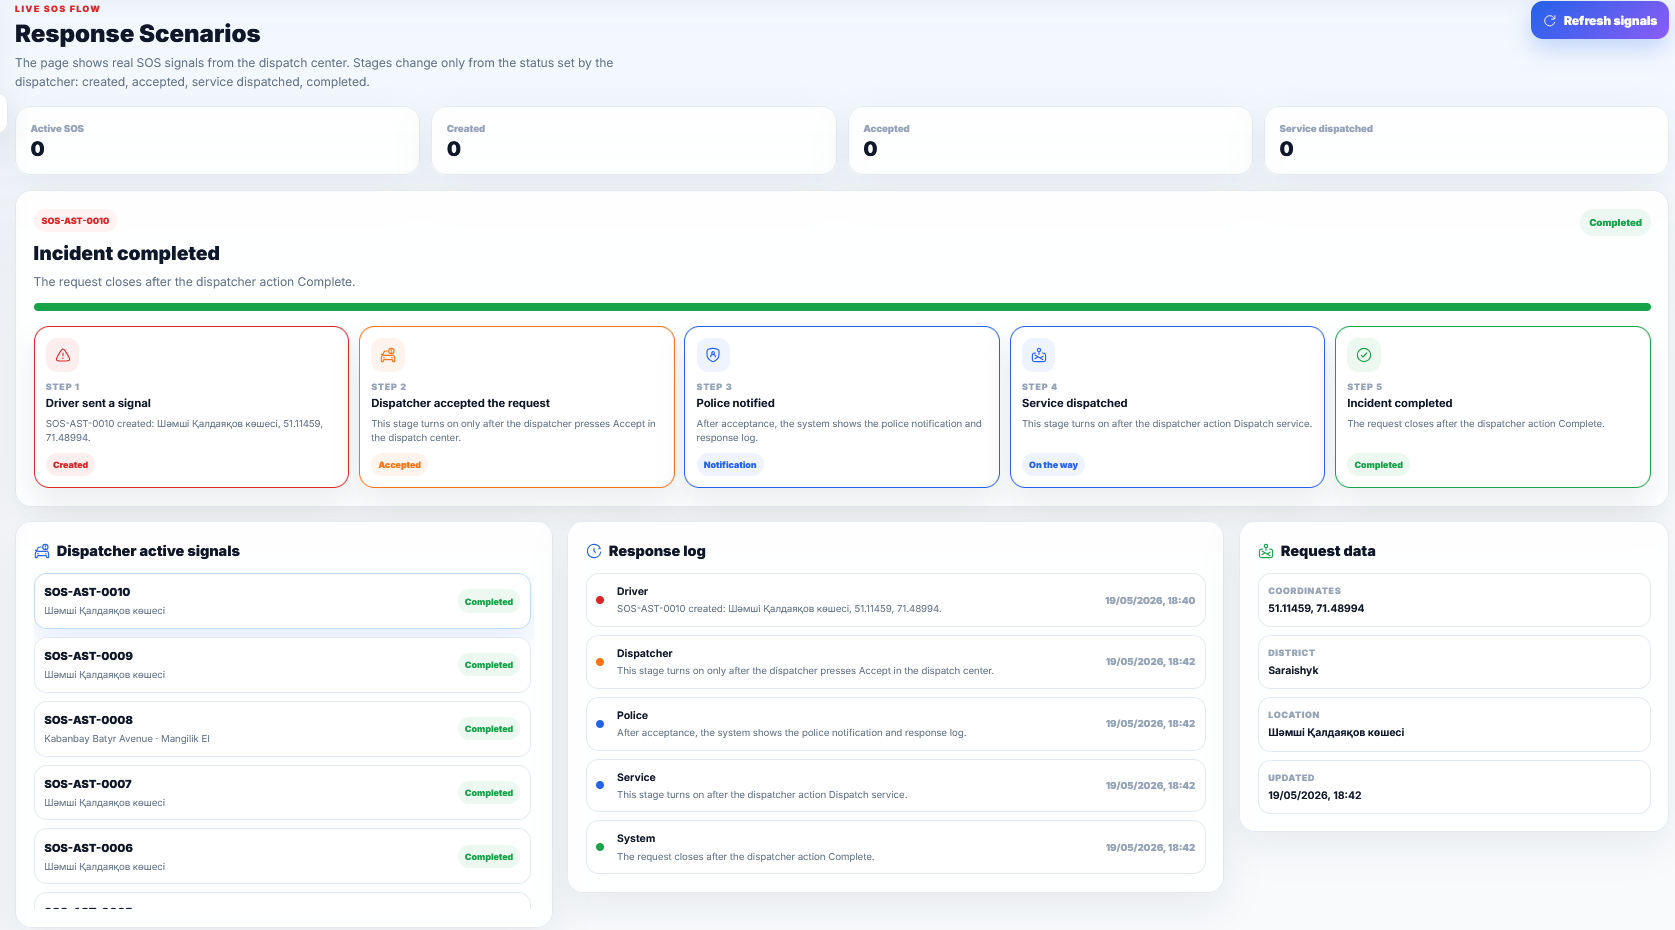
\includegraphics[width=\textwidth]{figures/response_scenarios_page.png}
\caption{Response Scenarios page}
\label{fig:appendix_response_scenarios}
\end{figure}

\begin{figure}[H]
\centering
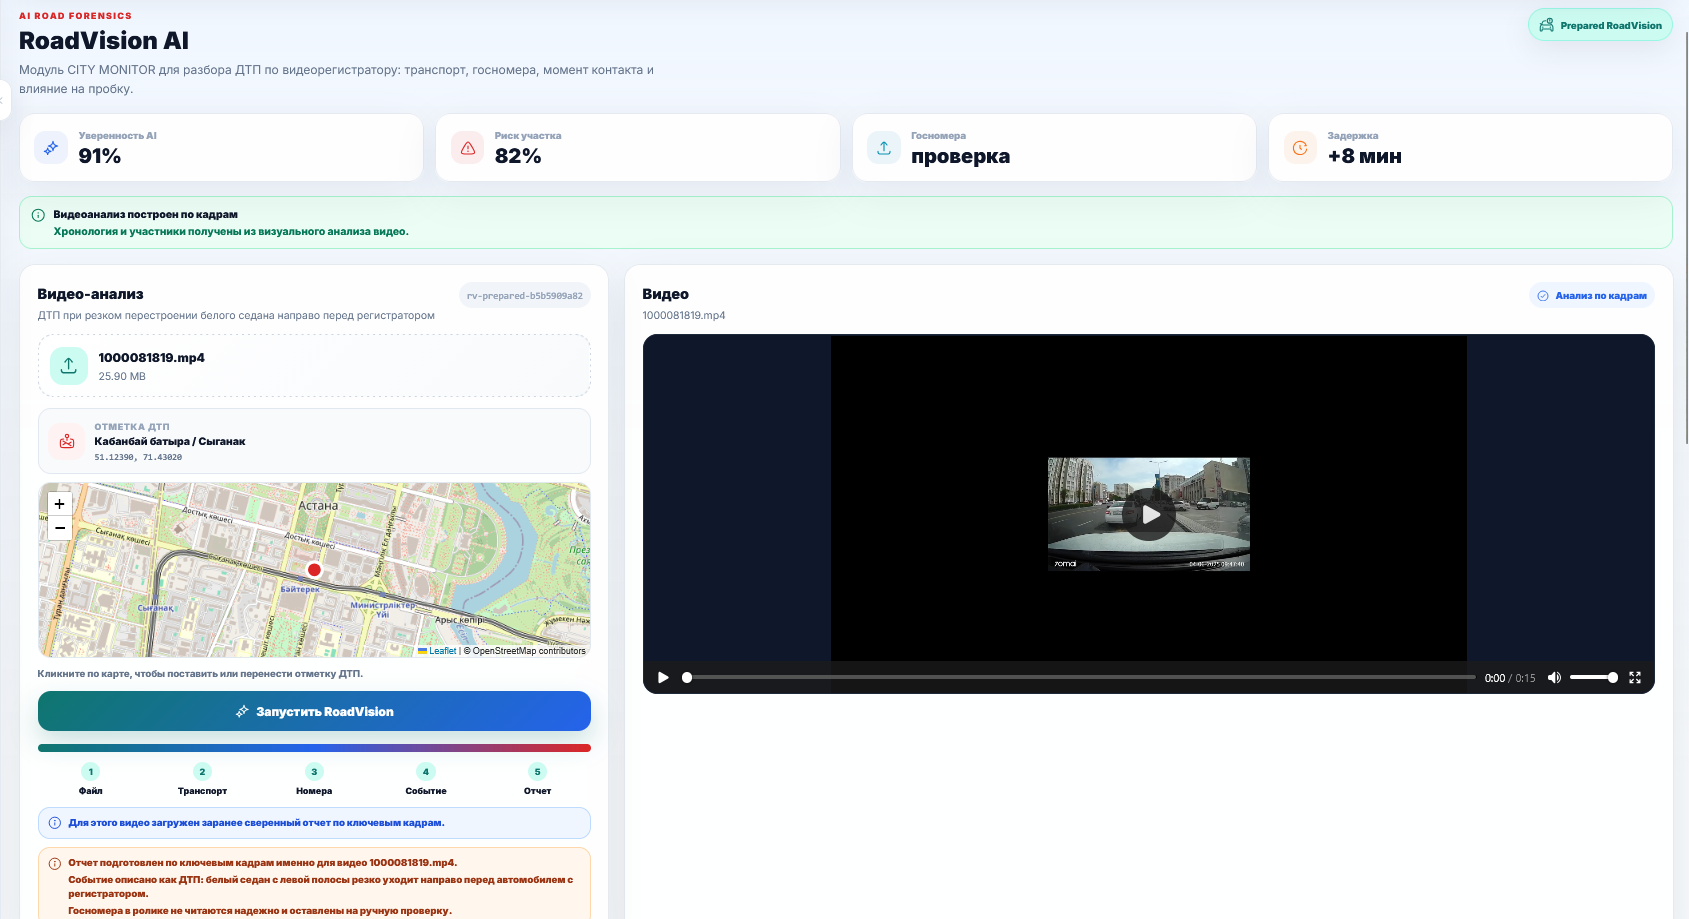
\includegraphics[width=\textwidth]{figures/roadvision_page.png}
\caption{RoadVision video upload and map point selection}
\label{fig:appendix_roadvision_upload}
\end{figure}

\begin{figure}[H]
\centering
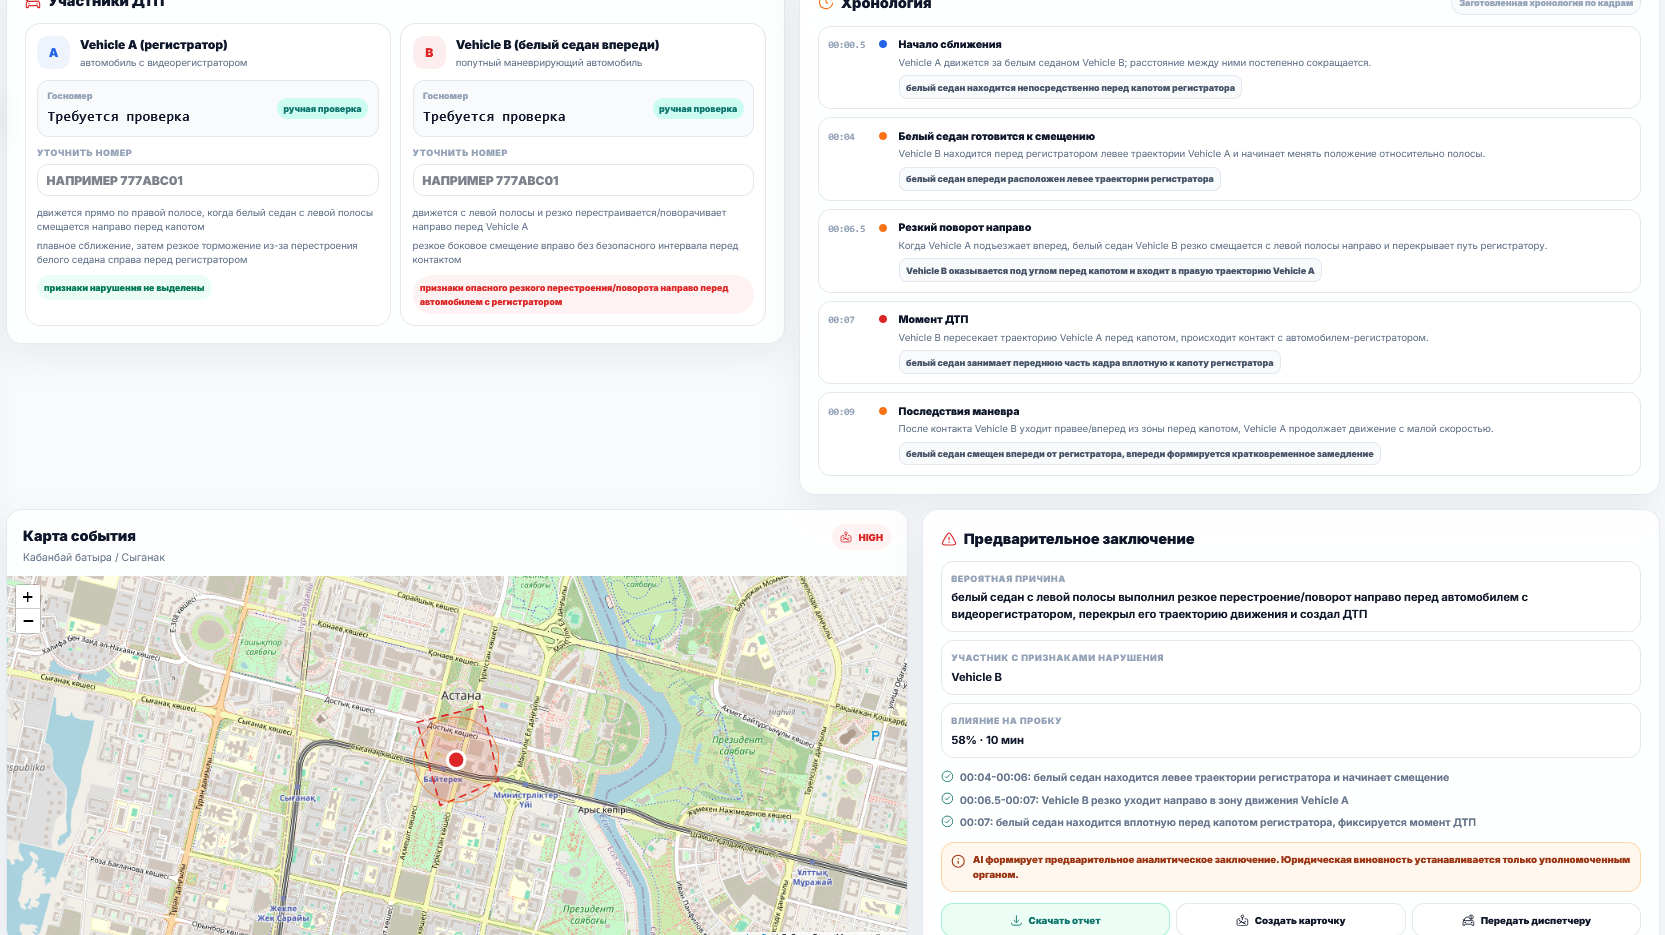
\includegraphics[width=\textwidth]{figures/roadvision_page_second.png}
\caption{RoadVision structured analysis result}
\label{fig:appendix_roadvision_result}
\end{figure}

\clearpage
\chapter{Testing Evidence}

Appendix C presents evidence of technical verification performed for the AstanaSafe system. Testing was included to confirm that the main project modules can be demonstrated without critical errors, the implemented backend services work correctly, and the frontend build process is completed successfully.

For the backend, automated tests were used. The checks covered password reset behavior, RoadVision processing functions, spatial risk analysis helpers, and AI forecast logic. These checks were selected because they represent important backend functions that support the analytical and operational parts of the system.

The backend passed 25 tests without errors. This result does not prove that the system solves every possible road safety problem, but it confirms that the tested backend service functions work as expected and that the backend logic is stable enough for project demonstration.

\begin{figure}[H]
\centering
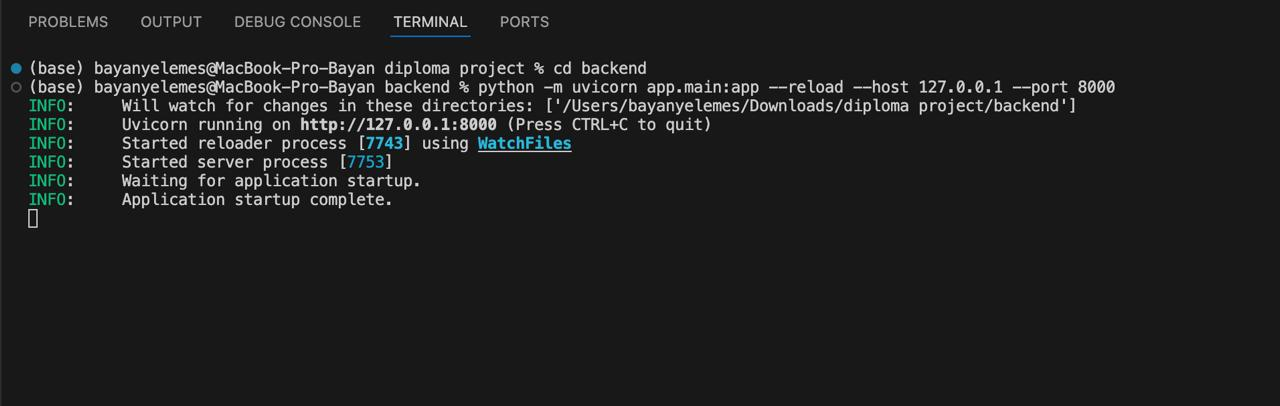
\includegraphics[width=\textwidth]{figures/backend_tests_passed.jpeg}
\caption{Backend automated test result}
\label{fig:appendix_backend_tests}
\end{figure}

The frontend was verified by running a production build. This confirms that the React/Vite application can be compiled into static files suitable for deployment. This check is important because the dashboard contains many interconnected pages, map components, charts, modals, and role-based views.

\begin{figure}[H]
\centering
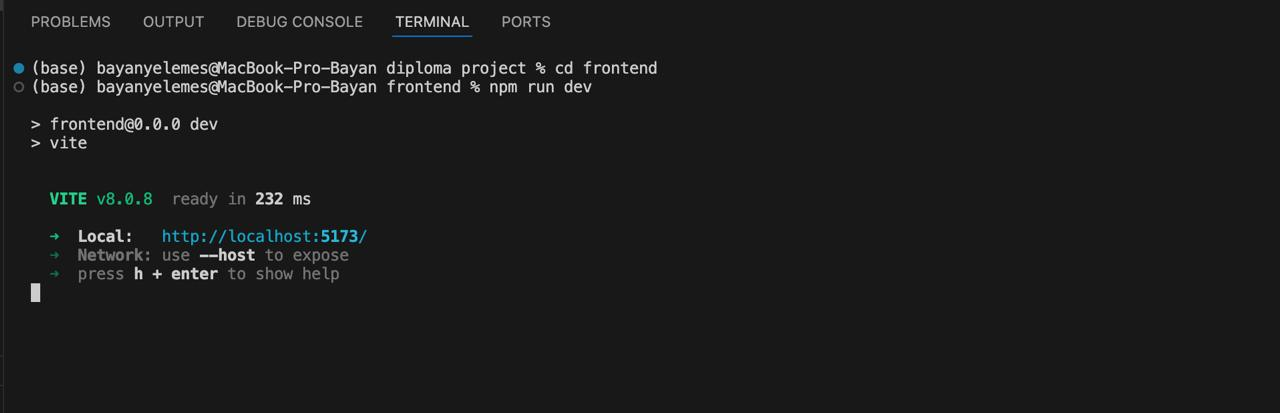
\includegraphics[width=\textwidth]{figures/frontend_build_success.jpeg}
\caption{Frontend production build result}
\label{fig:appendix_frontend_build}
\end{figure}

AstanaSafe was validated through both interface review and technical verification. The testing evidence confirms that the project can be presented not only as a user interface prototype, but also as a working web application with verified backend and frontend behavior.

\end{document}
